\documentclass[8pt, a4paper, fleqn, landscape]{scrartcl}
\usepackage[utf8]{inputenc}
\usepackage[ngerman]{babel}
\usepackage{ulem}

\usepackage{hyperref}

%Layout
\usepackage{multicol, geometry, xcolor}
\geometry{margin=1cm}
\parindent 0pt
\pagestyle{empty}

\newlength{\breite}
\setlength{\breite}{0.5pt}
\setlength{\columnseprule}{\breite}

\usepackage{graphicx}

\usepackage{tikz}
\usepackage{scalerel} %maybe not needed



%Mathematik-Pakete
\usepackage{amsmath, amstext, amssymb, mathtools, esint, polynom}
\usepackage{bm}
\allowdisplaybreaks %Seitenumbruch in align-Umgebung erlauben


% Farbe der Boxen für Titel / Untertitel
\definecolor{section}{RGB}{79,148,205}
\definecolor{subsection}{RGB}{135,206,250}
\definecolor{titletext}{RGB}{0,0,0}


% section color box
\setkomafont{section}{\mysection}
\newcommand{\mysection}[1]{%
	\Large\sffamily
	\setlength{\fboxsep}{0cm}%already boxed
	\colorbox{section}{%
		\begin{minipage}{\linewidth}%
			\vspace*{2pt}%Space before
			\leftskip2pt %Space left
			\rightskip\leftskip %Space right
			{\color{titletext} #1}
			\vspace*{1pt}%Space after
		\end{minipage}%
}}
% subsection color box
\setkomafont{subsection}{\mysubsection}
\newcommand{\mysubsection}[1]{%
	\Large\sffamily
	\setlength{\fboxsep}{0cm}%already boxed
	\colorbox{subsection}{%
		\begin{minipage}{\linewidth}%
			\vspace*{2pt}%Space before
			\leftskip2pt %Space left
			\rightskip\leftskip %Space right
			{\color{titletext} #1}
			\vspace*{1pt}%Space after
		\end{minipage}%
}}

				
\providecommand{\diff}{\mathop{} \! \mathrm{d}}

%new commands 
\newcommand{\const}{\mathrm{const}} 
\newcommand{\e}{\mathrm{e}}


%Informationen für den Befehl maketitle
\title{Physik}
\subtitle{Sammlung, gegliedert nach Modul}
\author{Fabian Suter, \today}
\date{{\small \url{https://github.com/FabianSuter/Physik.git}}}
 
\begin{document}

	\begin{multicols*}{3}
		\maketitle
	 
		% TODO: bei Gelegenheit alle Einheitenlisten mit \rule{0pt}{10pt} o.ä. überprüfen (passt die Zeilenhöhe an)

		%TODO: Auskommentieren nach Einfügen Modul 2
		% \section{Statik}
		
	\subsection{Schwerkraft (Gewichtskraft)}
	
		$$ \boxed{ \text{Allgemein:} \quad F_G = G \cdot \frac{m_1 \cdot m_2}{r^2} }$$
		$$ \boxed{ \text{Erde:} \quad  F_G = G \cdot \frac{m_E \cdot m}{r_E^2} = m \cdot g }$$ 
		
		\begin{tabular}{clc}
			$F_G$ & Gewichtskraft         & $[F_G] = \mathrm{\frac{kg \, m}{s^2} = N}$ \\
			$G$   & Gravitationskonstante & $6.67 \cdot 10^{-11} \mathrm{\frac{m^3}{kg \, s^2}}$ \\ 
			$m_i$ & Massen der Körper     & $[m] = \mathrm{kg}$ \\
			$r$   & Abstand der Massen    & $[r] =\mathrm{m}$ \\
			$g$   & Erdbeschleunigung     & $9.81 \mathrm{\frac{m}{s^2}}$ \\
			$m_E$ & Masse der Erde        & $5.972 \cdot 10^{24} \, \mathrm{kg} $ \\
			$r_E$ & Erdradius             & $6.378 \cdot 10^6 \, \mathrm{m}$ \\
		\end{tabular}
		
	\subsection{Normalkraft (Kontaktkraft)}
		(Sekundär-) Kraft, welche sich so anpasst, dass in Ruhe ein Kräftegleichgewicht herrscht: \\
		\\
		$\boxed{ F_G = -F_N}$ \qquad $\Rightarrow$ im Gleichgewicht auf horizontaler Oberfläche
				
	\subsection{Zerlegung von Kräften}
		Kraftvektoren kann man komponentenweise aufteilen: \\
		\\
		\begin{minipage}{0.6\linewidth}
			\begin{tikzpicture}
				[
				x=1cm, y=1cm, scale=0.7, font=\footnotesize, >=latex 
				%Voreinstellung für Pfeilspitzen
				]
				
				%Raster im Hintergrund
				\draw[step=1, gray, very thin] (0,0) grid (5.5,3.5);
				
				%Länge x Achse
				\draw [-latex] (0,0) -- ++(5.5,0) node[below, scale=1.2] {$x$};
				
				%Länge y Achse
				\draw [-latex] (0,0) -- ++(0,3.5) node[left, scale=1.2] {$y$};
				
				%Winkel
				\filldraw[fill=green!20!white, draw=green!50!black, thick] (1,1) -- (2.5,1) arc (0:26.56:1.5) -- cycle node[midway, below, green!50!black, scale=1.4, yshift=3pt, xshift=5pt] {$\alpha$};		
				
				%Vektor a
				\draw[-latex, very thick] (5,1) -- (5,3) node [midway, right, scale=1.2] {$\vec{F}_y$} node (Fy) {}; 
				%Vektor b
				\draw[-latex, very thick] (1,1) -- (5,1) node [midway, below, scale=1.2] {$\vec{F}_x$} node (Fx) {};

				%\draw[dashed] (a.center) -- ++ (3,0) node (c) {};
				%\draw[dashed] (b.center) -- ++ (2,3);
				\draw[very thick, red, -latex] (1,1) -- (Fy.center) node [midway, above, scale=1.2] {$\vec{F}$} node (F) {};
			\end{tikzpicture}
		\end{minipage}
		\hfill
		\begin{minipage}{0.6\linewidth}
			$\vec{F} = \vec{F}_x + \vec{F}_y + \vec{F}_Z$ \\	
			\\
			\textbf{hilfreich beim Lösen \\
			von Aufgaben!} \\
		\end{minipage}
		
	\subsection{Gleichgewichtsbedingungen für Massepunkte}
		Der Massepunkt erfährt keine Beschleunigung \\
		$\Rightarrow$ Summe aller wirkenden Kräfte ist 0 
		
		$$ \boxed{ \vec{R} = \sum \limits_{i = 1}^n \vec{F}_i = \vec{0} \qquad \Rightarrow \text{komponentenweise} }$$
		
		$$ \boxed{ \sum \limits_{i = 1}^n \vec{F}_x = \vec{0}  \qquad  \sum \limits_{i = 1}^n \vec{F}_y = \vec{0}  \qquad  \sum \limits_{i = 1}^n \vec{F}_z = \vec{0} } $$ 
			
	\subsection{Haftreibung / Gleitreibung}
	
		\subsubsection{Trockene Festkörperreibung}
	
			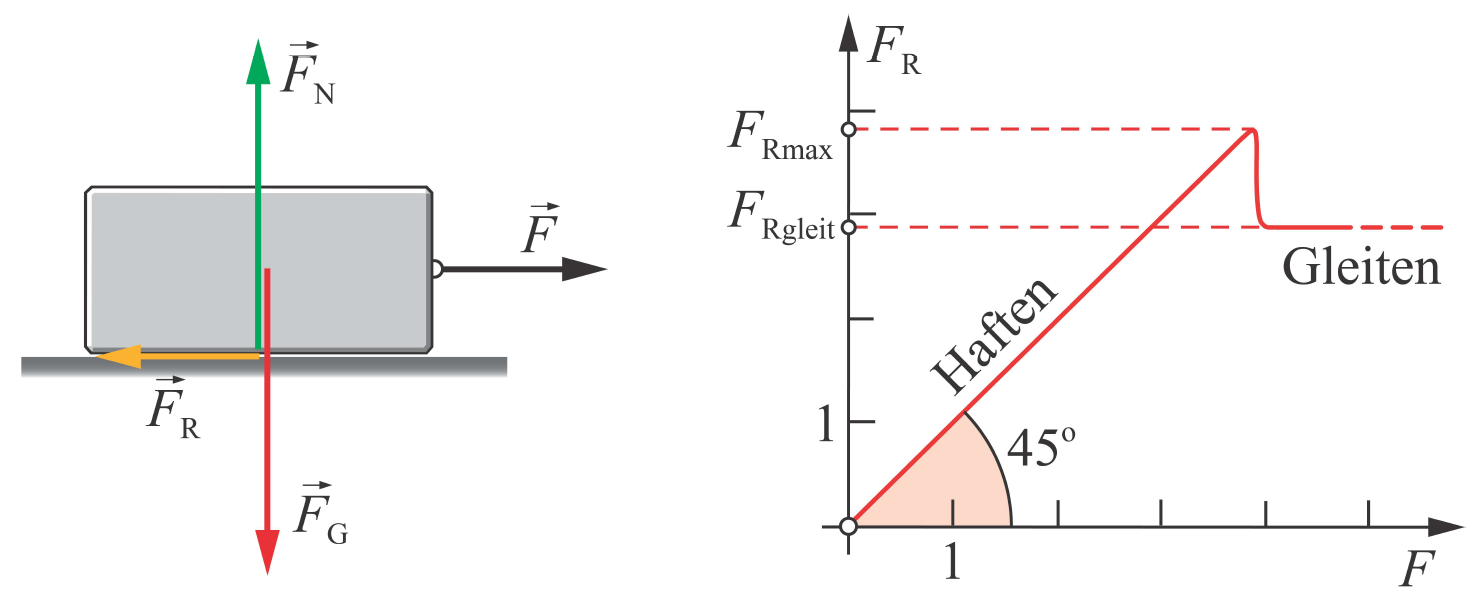
\includegraphics[width=0.7\linewidth]{Bilder/reibung} \\
		
			\begin{minipage}{0.65\linewidth}
				$$ \boxed{ \text{Haftreibung:} \quad \vec{F}_{R,max} = \mu_H \cdot \vec{F}_N } $$ 
				
				$$ \boxed{ \text{Gleitreibung:} \quad \vec{F}_{Gleit} \approx \mu_G \cdot \vec{F}_N } $$
			\end{minipage}
			\hfill
			\begin{minipage}{0.3\linewidth}
				$$ \boxed{ \vert \vec{F}_R \vert \leq \vert \vec{F}_{R,max} \vert } $$ \\
			\end{minipage}
		
			\begin{tabular}{lll}
				$\vec{F}_R$ & Reibungskraft & $[\vec{F}_R] = \mathrm{N}$ \\
				$\vec{F}_{R,max}$ & Haftreibungskraft & $[\vec{F}_{R,max}] = \mathrm{N}$ \\
				$\vec{F}_{Gleit}$ & Gleitreibungskraft & $[\vec{F}_{Gleit}] = \mathrm{N}$ \\
			\end{tabular}

		\subsubsection{Viskose Reibung}
			Sobald Schmiermittel zum Einsatz kommen, ist die Reibungskraft abhängig von der Grösse der Berührungsfläche: \\
			\\
			Bei gleicher Normalkraft $\vec{F}_N$ ist bei 
			
			\begin{tabular}{ll}
				$\bullet$ & kleinerem Flächendruck die Reibung kleiner \\
				$\bullet$ & grösserem Flächendruck die Reibung grösser \\
			\end{tabular}
		
	\subsection{Starre Körper}
	
		\begin{tabular}{ll}
			$\bullet$ & Ein starrer Körper wird durch angreifende Kräfte \\
			& nicht deformiert \\
			$\bullet$ & Bei einem starren Körper kann die Kraft entlang ihrer  \\
			& Wirkungslinie \underline{beliebig} verschoben werden \\
		\end{tabular}
	
	\subsection{Addition von Kräften}
		
		\subsubsection{Spezialfall: Ebene Kräftegruppe für schiefe Wirkungslinie}
			Kräfte entlang ihrer Wikungslinie verschieben \\
			$\Rightarrow$ Im Schnittpunkt vektorielle Addition der Kräfte durchführen, um die resultierende Kraft zu erhalten. \\
			\\
			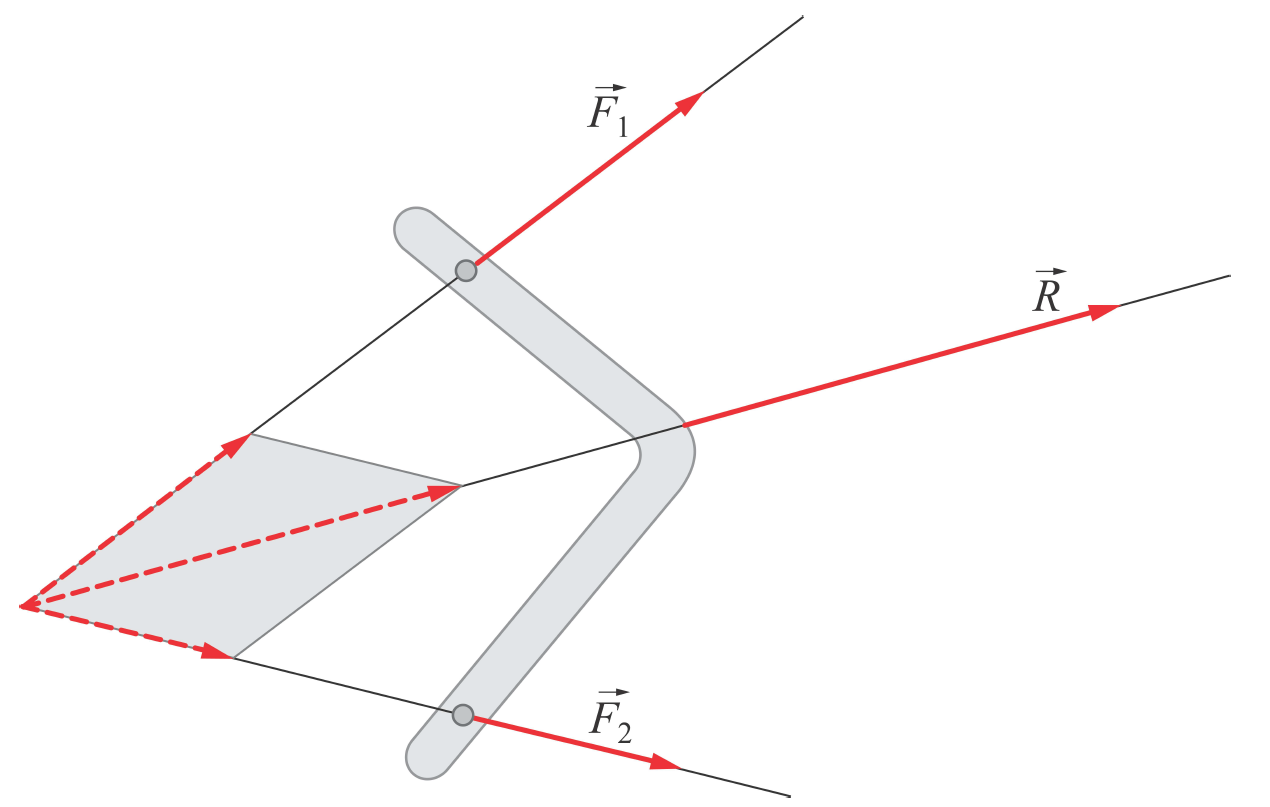
\includegraphics[width=0.7\linewidth]{Bilder/schneidende_wirkungslinien} \\
			\\
			Dieses Verfahren kann auch mehrfach angewendet werden!

		\subsubsection{Spezialfall: Ebene Kräftegruppe für parallele Wirkungslinie}
			Zwei sich zu null addierende Hilfskräfte hinzufügen ($\vec{H}_1 \; , \; \vec{H}_2$) \\
			\\	
			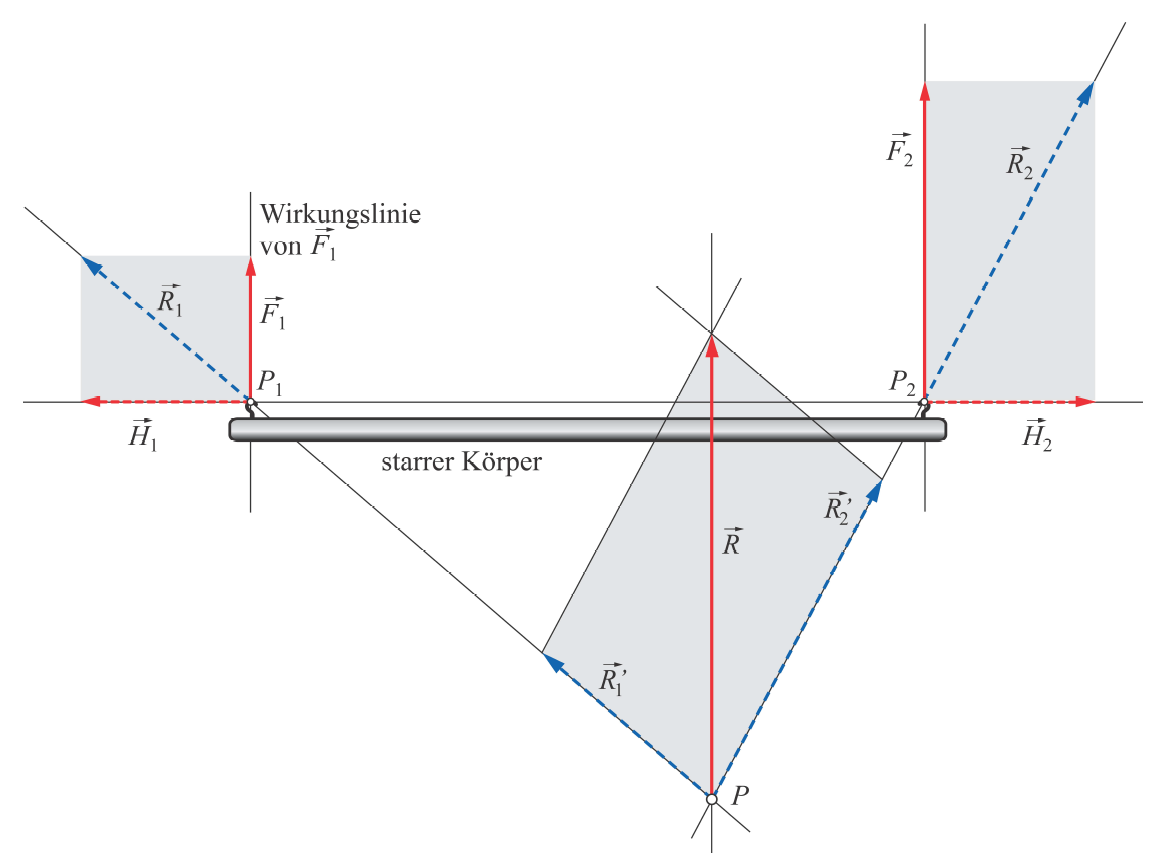
\includegraphics[width=0.7\linewidth]{Bilder/parallele_wirkungslinien}

		\subsubsection{Spezialfall: Ebene Kräftegruppe für parallel, entgegengesetzt und gleich grosse Kräfte}
	
			Kräftepaare können in andere Kräftepaare umgewandelt  werden, aber \underline{niemals zu einer} resultierenden Kraft $\vec{R}$ vereinfacht werden. \\
			\\
			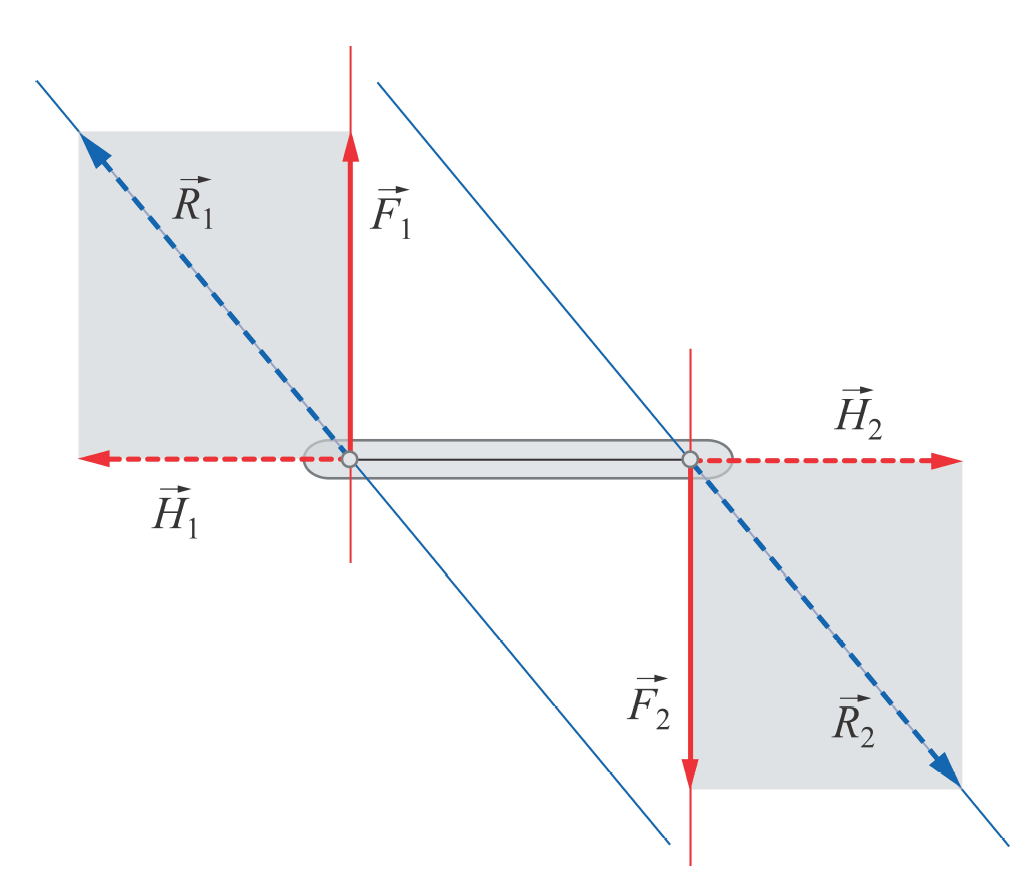
\includegraphics[width=0.7\linewidth]{Bilder/kraeftepaar_wirkungslinien}
		
	\subsection{Drehmoment}
		Eine Drehwirkung auf einen starren Körper lässt sich auf zwei \\
		verschiedene Arten und Weisen erzeugen: \\
		\\
		\begin{tabular}{ll}
			$\bullet$ & Kräftepaar \\
			$\bullet$ & einzelne Kraft und Bezugspunkt (Drehzentrum) \\
		\end{tabular}
		
		\begin{minipage}{0.48\linewidth}
			\begin{tikzpicture}
				[
				x=1cm, y=1cm, scale=0.5, font=\footnotesize, >=latex 
				%Voreinstellung für Pfeilspitzen
				]
				%Raster im Hintergrund
				%\draw[step=1, gray, very thin] (-5.5,-5.5) grid (5.5,5.5);
				\draw[thick, gray] (0, 0) circle(3.5);
				\draw[dashed] (2,3.5) -- (2,-3.5) node [midway, left, yshift=-1.2cm] {$Wirkungslinie$};
				\draw[-latex, draw=blue!50!black, very thick, rotate = -90] (1,0)--(1,0) arc(0:-250:1) 
								node [midway, above, xshift=-1.3pt, yshift=0, blue!50!black] {$\vec{M}$} {};
				\fill[black] (0, 0) circle(3.5pt) node [midway, above, yshift=7pt] {$Drehachse$};
				\begin{scope}[xshift=2cm, yshift=0cm, rotate=0, scale=1]
					%Kräfte
					\draw [-latex, very thick, green!50!black] (0,0) -- ++(0,-2) node[midway, left] {$\vec{F}{'}$};
					\fill [blue!70!white](0,0) circle (0.1) node[midway, right] {$P'$};;
				\end{scope}		
				\begin{scope}[xshift=2cm, yshift=0cm, rotate=90, scale=1]  		
					\draw [thick](-0.3,0) -- (-0.3,0.3) -- (0,0.3);
				\end{scope}	
				\begin{scope}[xshift=2cm, yshift=2.87228cm, rotate=0, scale=1]
					%Kräfte
					\draw [-latex, very thick, green!50!black] (0,0) -- ++(0,-2) node[midway, left] {$\vec{F}$};
					\fill [blue!70!white](0,0) circle (0.1) node[midway, right] {$P$};;
				\end{scope}	
				\draw[-latex, very thick, red] (0,0) -- ++(2,0) node[midway, below] {$\vec{r}$};
			\end{tikzpicture}
			\\
		\end{minipage}
		\hfill
		\begin{minipage}{0.48\linewidth}
			$ \vert \vec{M} \vert = \vert \vec{r} \times \vec{F} \vert = a \cdot \vert \vec{F} \vert  $	\\
			\\
			Die Länge a muss \textbf{senkrecht} zur wirkenden Kraft sein!
		\end{minipage}

		\begin{tabular}{lll}
			$\vec{M}$ & Drehmoment & $[M] = \mathrm{Nm}$ \\
			$\vec{r}$ & Abstandsvektor & $[r] = \mathrm{m}$ \\
			$\vec{F}$ & Angreifende Kraft & $[F] = \mathrm{N}$ \\
		\end{tabular}

	\subsection{Gleichgewichtsbedungungen für starre Körper}
		
		$ \sum \limits_{i = 1}^n \vec{F}_i = \vec{0}$  \qquad  $ \sum \limits_{i = 1}^m \vec{M}_i = \vec{0} $  \qquad $\Rightarrow$ komponentenweise
	
	\subsection{Gleichgewichts-Arten}	
		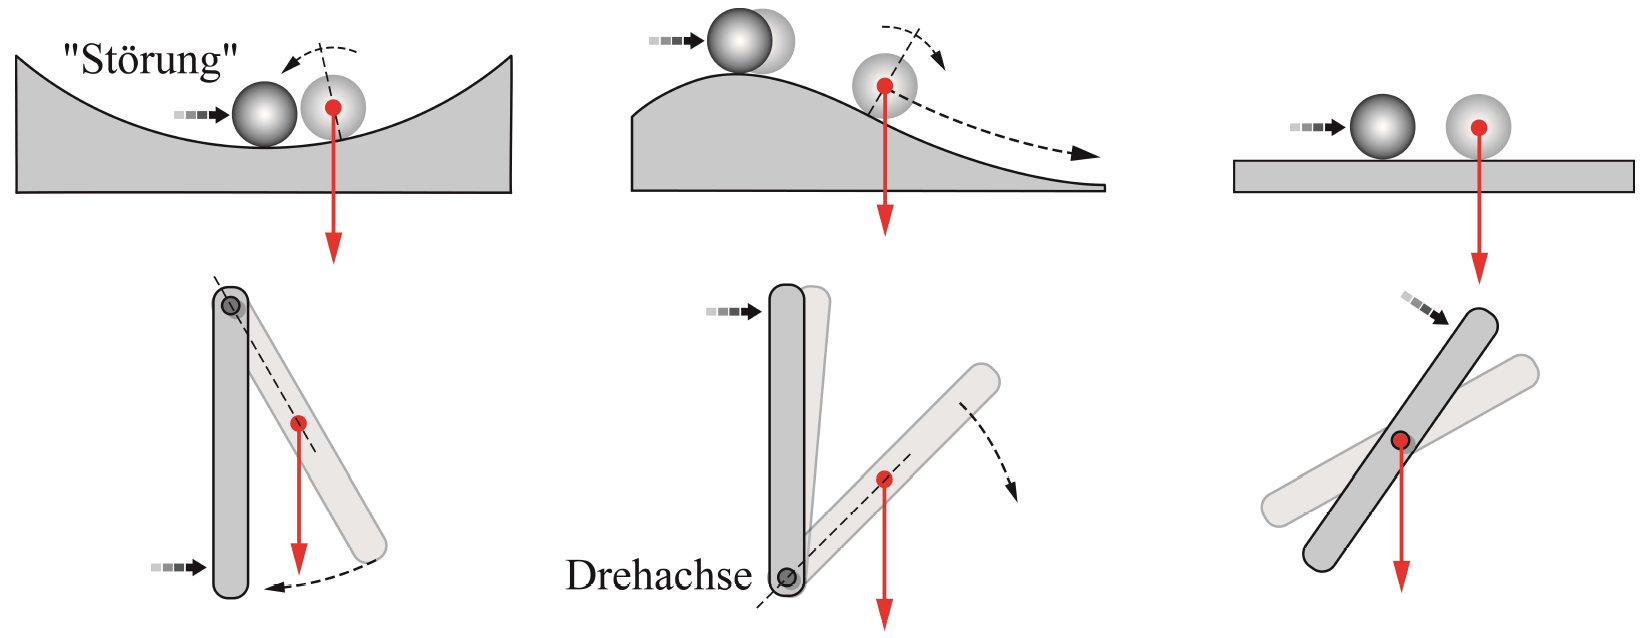
\includegraphics[width=0.95\linewidth]{Bilder/gleichgewichte} \\
		\\
		\begin{minipage}{0.3\linewidth}
			\center{stabil}
		\end{minipage}
		\hfill
		\begin{minipage}{0.3\linewidth}
			\center{labil}
		\end{minipage}
		\hfill
		\begin{minipage}{0.3\linewidth}
			\center{indifferent}
		\end{minipage}

	\subsection{Deformierbare Körper}
		
		\subsubsection{Spannungen}
			\textbf{Zugspannung $\sigma$} \\
				\\
				senkrecht wirkende Kraft pro Flächeneinheit \\
				Wenn $\sigma < 0$ spricht man von \textbf{Druck} 
				
				$$ \boxed{ \sigma = \frac{F_{\perp}}{A} } \qquad [\sigma] = \mathrm{\frac{N}{m^2}}$$ 

			\textbf{Schubspannung $\tau$ (Scherung)} \\
				\\
				parallel wirkende Kraft pro Flächeneinheit 
				
				$$ \boxed{ \tau = \frac{F_{\shortparallel}}{A} } \qquad [\tau] = \mathrm{\frac{N}{m^2}}$$

		\subsubsection{Dehnung $\epsilon$ (Hook'sches Gesetz)}
			$$ \boxed{ \epsilon = \frac{1}{E} \cdot \sigma = \frac{1}{E} \cdot \frac{F_{\perp}}{A} = \frac{\Delta \, l}{l} } $$ 

			\begin{tabular}{c l c}
				$\epsilon$ & Dehnung & $[\epsilon] = 1$ \\
				$E$ & Elastizitätsmodul (Materialeigenschaft) & $[E] = \mathrm{\frac{N}{m^2}}$ \\
				$l$ & Länge des Körpers vor Dehnung & $[l] = \mathrm{m}$ \\
				$\Delta \, l$ & Längenunterschied bei Dehnung & $[\Delta \, l] = \mathrm{m}$ \\
				$\sigma$ & Zugspannung & $[\sigma] = \mathrm{N}$ \\
				$A$ & Querschnittsfläche & $[A] = \mathrm{m^2}$ \\
				\\
			\end{tabular}
			
			$\Rightarrow$ \textbf{Das Hook'sche Gesetz gilt nur, solange die Deformation linear-elastisch ist!}

			%todo: Bild von Elastizität finden und einfügen

		\subsubsection{Querkontraktion $\epsilon_q$}
			Wird ein Stab gedehnt (länger), so wird er automatisch auch dünner \\		
			
			$$ \boxed{ \epsilon_q = \frac{\Delta \, d}{d} = - \mu \, \epsilon } \qquad \mu \in (0 \, ; \, 0.5)$$ \\
			
			\begin{tabular}{c l c}
				$\epsilon_q$ & Querkontraktion & $[\epsilon_q] = 1$ \\
				$d$ & Ursprüngliche Dicke des Materials & $[d] = \mathrm{m}$ \\
				$\Delta d$ & Dicken-Änderung & $[ \Delta \, d] = \mathrm{m}$ \\
				$\epsilon$ & (Längs-) Dehnung & $[\epsilon] = 1$ \\
				$\mu$ & Poisson-Zahl (Materialeigenschaft) & $[\mu] = 1$ \\
			\end{tabular}
		
		\subsubsection{Kompression $\frac{\Delta \, V}{V}$}
			Ein Körper wird von allen Seiten mit dem gleichen Druck belastet, sodass sich sein Volumen verkleinert 
			
			$$ \boxed{ \frac{\Delta \, V}{V} = - \kappa \cdot \Delta \, p } \qquad \Big( K = \frac{1}{\kappa} \Big) $$ \\ 
			
			\begin{tabular}{c l c}
				$V$ & Ursprüngliches Volumen des Körpers & $[V] = \mathrm{m^3}$ \\
				$\Delta V$ & Volumenänderung & $[\Delta V] = \mathrm{m^3}$ \\
				$\kappa$ & Kompressibilität & $[\kappa] = \mathrm{\frac{m^2}{N}}$ \\
				$\Delta \, p$ & Druckänderung & $[\Delta \, p] = \mathrm{\frac{N}{m^2} = Pa}$  \\ 
			\end{tabular}
			
			$$ \boxed{ \text{Würfel:} \quad \Rightarrow \kappa = \frac{3}{E} (1 - 2 \, \mu) }$$ 
			
			\textbf{Völlig inkompressibler Körper:} $\kappa = 0$  \qquad $K = \infty$ \qquad $\mu = 0.5$

		\subsubsection{Schubbeanspruchung (Scherung)}
		
			$$ \boxed{ \gamma = \frac{1}{G} \, \tau }$$ 
			
			$$ \boxed{ G = \frac{E}{2(1 + \mu)}  \quad \text{(gilt für isotrope Materialen)} } $$\\

			\begin{tabular}{c l c}
				$\gamma$ & Scherwinkel & $[\gamma] = \; ^\circ $ \\
				\rule{0pt}{10pt}$G$ & Schubmodul; Gleitmodul; Torsionsmodul & $[G] = \mathrm{\frac{N}{m^2}}$ \\
				\rule{0pt}{10pt}$\tau$ & Schubspannung & $[\tau] = \mathrm{\frac{N}{m^2}}$ \\
				\rule{0pt}{10pt}$E$ & Elastizitätsmodul (Materialeigenschaft) & $[E] = \mathrm{\frac{N}{m^2}}$ \\
				$\mu$ & Poisson-Zahl (Materialeigenschaft) & $[\mu] = 1$ \\
			\end{tabular}

		\subsubsection{Torsionsfeder}
		
			$$ \boxed{ M = c \cdot \varPhi \quad \quad c = \frac{\pi G r^4}{2l} }$$ 

			\begin{tabular}{c l c}
				$M$ & Drehmoment & $[M] = Nm$ \\
				$c$ & Auslenkkonstante & $[c] = $ \\
				$\varPhi$ & Auslenkwinkel & $[\varPhi] = \; ^\circ $ \\
				$G$ & Schubmodul & $[G] = \mathrm{\frac{N}{m^2}}$ \\
				$r$ & Radius der Feder & $[r] = m$ \\
				$l$ & Länge der Feder & $[l] = m$ \\
			\end{tabular}

		\subsubsection{Schraubenfeder}
		
			$$ \boxed{ F = c \cdot \Delta l \quad \quad c = \frac{G r^4}{4nR^3} }$$ 

			\begin{tabular}{c l c}
				$F$ & Kraft & $[F] = N$ \\
				$c$ & Auslenkkonstante & $[c] = $ \\
				$\Delta l$ & Längenänderung & $[\Delta l] = m$ \\
				$G$ & Schubmodul & $[G] = \mathrm{\frac{N}{m^2}}$ \\
				$r$ & Drahtradius der Feder & $[r] = m$ \\
				$R$ & Windungsradius der Feder & $[R] = m$ \\
				$n$ & Anzahl Windungen & $[n] = $ \\
			\end{tabular}

		\subsubsection{Blattfeder}
		
			$$ \boxed{ z = \frac{4l^3}{E \cdot b \cdot h^3}F }$$ 

			\begin{tabular}{c l c}
				$F$ & Kraft & $[F] = N$ \\
				$z$ & Verbiegung & $[z] = m$ \\
				$l$ & Längenänderung & $[l] = m$ \\
				$E$ & Elastizitätsmodul & $[E] = \mathrm{\frac{N}{m^2}}$ \\
				$b$ & Breite des Querschnitts & $[b] = m$ \\
				$h$ & Höhe des Querschnitts & $[h] = m$ \\
			\end{tabular}

	\subsection{Schiefe Ebene (mit Seil)}
		\begin{tikzpicture}
			[
			x=1cm, y=1cm, scale=0.85, font=\footnotesize, >=latex 
			%Voreinstellung für Pfeilspitzen
			]
			
			%Raster im Hintergrund
			%\draw[step=1, gray, very thin] (0,0) grid (7,6);	

			%Grunddreieck	
			\draw [fill=gray!20] (0,0) -- (7,0) -- (7,4.04145) -- (0,0);
			
			%Winkel
			\filldraw[fill=blue!10, draw=blue!50!black, thick] (0,0) -- (1.5,0) arc(0:30:1.5) 
				node [midway, xshift=-10pt, yshift=-3, blue!50!black] {$\alpha$} {};
					
			\draw [very thick] (0,0) -- (7,0) -- (7,4.04145) -- (0,0);
					
			%Bezugssystem
			\begin{scope}[xshift=1cm, yshift=3cm, rotate=30, scale=1]
				%Länge x Achse
				\draw [-latex, thick] (0,0) -- ++(1,0) node[below, rotate=30] {$x$};
			
				%Länge y Achse
				\draw [-latex, thick] (0,0) -- ++(0,1) node[left, rotate=30] {$y$};
			\end{scope}
			%Alles was gedreht wurde (Masse m, Kräftevektoren, ...)
			\begin{scope}[xshift=3.464cm, yshift=2cm, rotate=30, scale=1.1]

				\coordinate (A) at (0.75,0.5);
				\coordinate (B) at (0.75,-1.5);
				
				%Rechteck
				\draw [fill=orange!20!white] (0,0) rectangle (1.5,1);
				\draw [orange, very thick] (0,0) rectangle (1.5,1) node [midway, right, xshift=3pt, yshift=3pt] {$m$} {} ;
				
				%Vektoren Kraft-Seil
				\begin{scope}[xshift=1.5cm, yshift=1cm, rotate=0, scale=1]
					\begin{scope}[xshift=0cm, yshift=0cm, rotate=0, scale=1]
						\filldraw[fill=green!10, draw=green!50!black, thick] (0,0) -- (1,0) arc(0:33.6900:1) 
							node [midway, left, xshift=0pt, yshift=-7, green!50!black] {$\beta$} {};
					\end{scope}
					\coordinate (C) at (1.5,0);
					\coordinate (D) at (1.5,1);
					%Rechter Winkel
					\draw [thick](1.2,0) -- (1.2,0.3) -- (1.5,0.3);
					\draw [-latex, very thick, purple] (0,0) -- ++ (C) node [midway, below] {$\vec{F}_{Sx}$} {};
					\draw [-latex, very thick, green!50!black] (C) -- ++ (0,1) node [midway, right] {$\vec{F}_{Sy}$} {};
					\draw [-latex, very thick, red] (0,0) -- ++ (D) node [midway, left] {$\vec{F}_S$} {};
					%Rechter Winkel
				
				\end{scope}	
				
				%Vektoren FN, FG, FH
				
				\begin{scope}[xshift=0cm, yshift=0, rotate=0, scale=1]
					\coordinate (A) at (0.75,0.5);
					\coordinate (B) at (0.75,-1.5);
					\begin{scope}[xshift=0.75cm, yshift=0.5cm, rotate=-120, scale=1]
						\filldraw[fill=blue!10, draw=blue!50!black, thick] (0,0) -- (1,0) arc(0:30:1) 
							node [midway, above, xshift=-1.5pt, yshift=0, blue!50!black] {$\alpha$} {};
					\end{scope}
					%Rechter Winkel
					\draw [thick](0.45,-1.5) -- (0.45,-1.2) -- (0.75,-1.2);  
					\draw [-latex, very thick, dashed, green!50!black] (B) -- (A) node [midway, right] {$\vec{F}_N$} {};
					\draw [-latex, very thick, green!50!black] (A) -- ++(0,2) node [midway, right] {$\vec{F}_N$} {};
					\draw [-latex, very thick, purple] (B) -- ++(-1.1547,0) node [midway, below] {$\vec{F}_H$} {};
					\draw [-latex, very thick, red] (A) -- ++(-1.1547,-2) node [midway, left] {$\vec{F}_G$} {};
					%Rechter Winkel
					\draw [thick](0.45,-1.5) -- (0.45,-1.2) -- (0.75,-1.2);  
				\end{scope}		    		
			\end{scope}
			
		\end{tikzpicture}
		\\
		\textbf{Wichtige Formeln und Zusammenhänge zur schiefen Ebene} \\
			\\
			\begin{tabular}{lll}
				$F = m \cdot a$  & $F_G = m \cdot g$ \\
				\\
				$F_N = m \cdot g \cdot \cos(\alpha)$ & 
				$F_H = m \cdot g \cdot \sin(\alpha)$ \\
			\end{tabular}

	\subsection{Rezept: Aufgaben zur Statik lösen}
	
	\begin{tabular}{ll}
		1. & Koordinatensystem festlegen  \\
		2. & Alle wirkenden Kräfte einzeichnen \\
		3. & Bezugspunkt P (Drehpunkt) festlegen \\
		& $\Rightarrow$ \textbf{Da wo viele Kräfte} (oder da wo sinnvoll) \\
		4. & Kräfte komponentenweise aufschreiben: $\sum \vec{F}_i = 0$ \\
		5. & Drehmomente M aufschreiben und gleichsetzen: $\overleftarrow{M} = \overrightarrow{M}$ \\
	\end{tabular}

	\vfill\null
	\pagebreak
		
		% %Code geputzt, Inhalt kontrolliert

		% \section{Kinematik}
			
	\subsection{Geradlinige Bewegung (1D)}
		Die Bewegung erfolgt entlang einer Gerade (keine Richtungsänderung) \\
		\\
		\begin{minipage}{0.48\linewidth}
			\begin{equation*}
				x(t) \quad  \underrightarrow{ \frac{d}{dt}} \quad  v(t) \quad  \underrightarrow{ \frac{d}{dt}} \quad a(t)  
			\end{equation*}
		\end{minipage}
		\hfill
		\begin{minipage}{0.48\linewidth}
			\begin{equation*}
				x(t) \quad \underleftarrow{\int dt} \quad v(t) \quad \underleftarrow{\int dt} \quad a(t)
			\end{equation*}
		\end{minipage}

		\subsubsection{Weg $x(t)$}
			Weg mit Zeit parametrisiert: $x = x(t)$ 

		\subsubsection{Geschwindigkeit $v(t) = \frac{\Delta \, x}{\Delta \, t}$}
		
			\begin{tabular}{lll}
				momentane Geschw.: & $\frac{d}{dt} x(t) = \dot{x}(t)$ & (Tangente) \\	
				\\
				mittlere Geschw.: & $\overline{v} = \frac{x_2 -x_1}{t_2 - t_1} =  \frac{x(t_2) - x(t_1)}{t_2 - t_1} $  & (Sekante) \\
			\end{tabular}

		\subsubsection{Beschleunigung $a(t) = \frac{\Delta \, v}{\Delta \, t}$}
			
			\begin{tabular}{ll}
				momentane Beschleunigung: & $\frac{d}{dt} v(t) = \dot{v}(t) = \ddot{x}(t)$ \\	
				\\
				mittlere Beschleunigung: & $\overline{a} = \frac{v_2 -v_1}{t_2 - t_1} =  \frac{v(t_2) - v(t_1)}{t_2 - t_1} $ \\
			\end{tabular}

		\subsubsection{Ruck $j(t)$}
		Änderung der Beschleunigung pro Zeiteinheit: $j(t) = \dot{a}(t) = \dddot{x}(t)$

	\subsection{Gleichförmige Bewegung $a(t) = 0$}
		\begin{tabular}{l}
			$a(t) = 0$ \\
			\\
			$v(t) = v_0 = \; \text{const}$ \\
			\\
			$x(t) = v_0 \cdot t + x_0 $ \\
		\end{tabular}
		
	\subsection{Gleichm. beschleunigte Bewegung $a(t) = $ konst}
		\begin{minipage}{0.48\linewidth}
			\textbf{Allgemein:} \\
				\\
				\begin{tabular}{l}
					$a(t) = a_0 = \text{const}$ \\
					\\
					$v(t) = a_0 \cdot t + v_0$ \\
					\\
					$x(t) = \frac{1}{2} \, a_0 \cdot t^2 + v_0 \cdot t + x_0$
				\end{tabular}
		\end{minipage}
		\hfill
		\begin{minipage}{0.48\linewidth}
			\textbf{Anwendungsfall: Freier Fall} \\
				\\
				\begin{tabular}{ll}
					$a(t) = -g = \text{const}$ \\
					\\
					$v(t) = -g \cdot t $ \\
					\\
					$x(t) = - \frac{1}{2} \, g \cdot t^2 + h_0$
				\end{tabular}
		\end{minipage}

		\subsubsection{Höchsten Punkt $x_{max}$ finden (Extremum)}
		
			Im Extremalpunkt gilt: $\frac{d}{dt} x(t) = v(t) \overset{!}{=} 0$ \\
			\\
			$0 \overset{!}{=} v(t_{max}) = -g \cdot t_{max} + v_0 $ \qquad \qquad $\Rightarrow t_{max} = \frac{v_0}{g}$ \\
			
			Durch einsetzen von $t_{max}$ in $x(t)$ erhält man die maximale Höhe: \\
			$x(t_{max}) = - \frac{1}{2}\, g \cdot t_{max}^2 + v_0 \cdot t_{max} + h_0 = - \frac{v_0^2}{2 \, g}\, + \frac{v_0^2}{g} + h_0 $

	\subsection{Beliebige Bewegung (2D)}
		
		\subsubsection{Geschwindigkeit (tangential zur Bahnkurve)}
		
			\begin{tabular}{ll}
				momentane Geschw.: & $ \vec{v} = \lim \limits_{\Delta t \rightarrow 0} \frac{\Delta \vec{r}}{\Delta t}  \frac{d}{dt} \vec{r} = \dot{\vec{r}}$ \\	
				\\
				mittlere Geschw.: & $\overline{\vec{v}} = \frac{\Delta \vec{r}}{\Delta t} = \frac{\vec{r}(t + \Delta t) - \vec{r}(t)}{\Delta t} $ \\
				\\
				Betrag: & $v = \vert \vec{v} \vert = \lim \limits_{\Delta t \rightarrow 0} \frac{ \vert \Delta \vec{r} \vert}{\Delta t} = \lim \limits_{\Delta t \rightarrow 0} \frac{\Delta s }{\Delta t} = \frac{d}{dt} s$ \\
			\end{tabular}

		\subsubsection{Beschleunigung}
			\begin{tabular}{ll}
				momentane Beschl.: & $ \vec{a} = \frac{d}{dt} \vec{v} = \dot{\vec{v}} = \frac{d^2}{d t^2} \vec{r} = \ddot{\vec{r}}$ \\	
				\\
				mittlere Beschl.: & $\overline{\vec{a}} = \frac{\Delta \vec{v}}{\Delta t} $ \\
			\end{tabular}
		
			\textbf{Die Beschleunigung kann ungleich null sein, auch wenn der Betrag der Geschwindigkeit konstant ist}

	\subsection{Bahnkurven}	
		Die Geschwindigkeitsänderung in einer Bahnkurve wird in zwei \\
		Komponenten aufgeteilt: \\
			$\Delta \vec{v}_{radial}$ \quad und \quad $\Delta \vec{v}_{tangential}$ \\
			\\
		Der tangentiale Anteil ändert ausschliesslich den Betrag der \\
		Geschwindigkeit $\vert \vec{v} \vert$ \\
		Der radiale Anteil ändert ausschliessich die Richtung der \\
		Geschwindigkeit $\vec{v}$ \\

		\begin{minipage}{0.45\linewidth}
			\begin{tikzpicture}
				[
				x=1cm, y=1cm, scale=0.6, font=\footnotesize, >=latex 
				%Voreinstellung für Pfeilspitzen
				]
				%Raster im Hintergrund
				%\draw[step=1, gray, very thin] (0,0) grid (5.5,5.5);
				\draw[thick] (0, 0) circle(2.5);
				\fill[black] (0, 0) circle(5pt) node [midway, above, yshift=7pt, scale=2] {$m$};
				\begin{scope}[xshift=2.5cm, yshift=0cm, rotate=0, scale=1]
					%Kräfte
					\draw [-latex, very thick, green!50!black] (0,0) -- ++(0,-2) node[midway, right, scale=1.2] {$\vec{a}_{tangential}$};
					\draw [-latex, very thick, purple] (0,0) -- ++(-1.5,0) node[midway, above, scale=1.2, xshift=-3pt] {$\vec{a}_{radial}$};
					\draw [-latex, very thick, orange] (0,0) -- ++(-1.5,-2) node[midway, left, scale=1.2] {$\vec{a}_{tot}$};
					\fill [blue!70!white](0,0) circle (0.1) node[midway, right, scale=2] {$P$};;
				\end{scope}		
			\end{tikzpicture}
		\end{minipage}
		\hfill
		\begin{minipage}{0.55\linewidth}
			$a_{tangential} = \frac{dv}{dt} = \dot{v}$ \\
			\\
			$a_{radial} = \frac{v^2}{r}$ \\
			\\
			$ \boxed { F_{zentripetal} = m \, \frac{v^2}{r} }$ \\
			\\
			$ \boxed{ (F_{zentri})^2 + (F_{bremsen})^2 = (F_R)^2 }$
		\end{minipage}

	\subsection{Gleichförmige Bewegung $a_{tangential} = 0$}
	
		\begin{minipage}{0.6\linewidth}
			\textbf{tangential (Tacho)} \\
				\\
				$a_{tangential} = 0$ \\
				\\
				$v(t) = v_0 = \text{const}$ \\
				\\
				$s(t) = v_0 \cdot t + s_0$ \\
		\end{minipage}
		\hfill
		\begin{minipage}{0.35\linewidth}
			\textbf{radial} \\
				\\
				$a_{radial} = \frac{v^2}{r}$ \\
				\\
				\\
				\\
				\\
		\end{minipage}

	\subsection{Gleichm. beschl. Bewegung $a_{tangential} = \text{konst}$}		
		\begin{minipage}{0.6\linewidth}
			\textbf{tangential (Tacho)} \\
				\\
				$a_{tangential} = a_0 = \text{const}$ \\
				\\
				$v(t) = a_{tangential} \cdot t + v_0 $ \\
				\\
				$s(t) = \frac{1}{2} \, a_{tangential} \cdot t^2 +  v_0 \cdot t + s_0$ \\
		\end{minipage}
		\hfill
		\begin{minipage}{0.35\linewidth}
			\textbf{radial} \\
				\\
				$a_{radial} = \frac{v^2}{r}$ \\
				\\
				\\
				\\
				\\
		\end{minipage}

		Die Gesamtbeschleunigung eines Systems $\vec{a}_{tot} = \vec{a}_{tangential} + \vec{a}_{radial} $ muss nicht zwingend konstant sein! Bei Änderungen der Richtung ändert die Gesamtbeschleunigung. 
	
	\subsection{Kreisbewegung}
		
		\subsubsection{Winkel $\phi$ (zurückgelegter Weg)}
		
		\begin{minipage}{0.5\linewidth}
			\begin{tikzpicture}
				[
				x=1cm, y=1cm, scale=1.0, font=\footnotesize, >=latex 
				%Voreinstellung für Pfeilspitzen
				]

				%Länge x Achse
				\draw [thick] (0,0) -- ++(2,0) node[below] {};
				\draw [thick] (1,0) node[below] {$r$};
				
				%Zahlen auf x-Achse
				\foreach \x in {0,2}
				\draw[shift={(\x,0)},color=black, thick] (0pt,2pt) -- (0pt,-2pt);
				
				%Winkelgugus
				\begin{scope}[xshift=0cm, yshift=0.25cm, rotate=0, scale=1]
					\filldraw[fill=white, thick] (0,0) -- (2,0) arc (0:30:2) -- cycle 
						node[midway, below, green!50!black, xshift=0pt, yshift=0pt] {};
					\filldraw[fill=white, thick] (0,0) -- (1,0) arc (0:30:1) -- cycle 
						node[midway, xshift=8pt, yshift=-1pt] {$\phi$};
				\end{scope}
				
				\draw [<->, thick] (2.25,0.25) arc (0:30:2.25) node[midway, right, xshift=0pt, yshift=0pt] {$S$};
			\end{tikzpicture}
		\end{minipage}
		\hfill
		\begin{minipage}{0.4\linewidth}
			$\boxed{ \text{Radiant: } \phi = \frac{s}{r} }$ 
		\end{minipage}

		\subsubsection{Winkelgeschwindigkeit $\omega= \frac{\phi}{t}$}
		
			$\omega := \lim \limits_{\Delta t \rightarrow 0} \frac{\phi(t + \Delta t) - \phi(t)}{\Delta t} = \frac{d \phi}{dt} = \dot{\phi}$ \\
			\\
			Der Betrag $v$ der (Bahn-) Geschwinndigkeit entspricht: $v = r \cdot \omega$ \\

			\begin{tabular}{ll}
				Umlaufzeit, Periode $T$ & Umlaufzeit für vollständige Umdrehung \\
				\\
				Drehzahl, Drehfrequenz $f$ & inverse Umlaufzeit   $f = \frac{1}{T}$ \\
				\\
				\\
			\end{tabular}
			
			\textbf{Wichtige Umrechnungsformeln} \\		 
				\\
				\boxed{
					\begin{tabular}{l c l l}
						$v = r \cdot \omega$ & $\Leftrightarrow$ & $\omega = \frac{v}{r}$ & \\		
						\\
						$f = \frac{1}{T}$ & $\Leftrightarrow$ & $T = \frac{1}{f}$ & \\
						\\
						$\omega = \frac{2 \, \pi}{T}$ & $\Leftrightarrow$ & $T = \frac{2 \, \pi}{f}$ & $\omega = \frac{2 \pi n}{60} $ \\
						\\
						$\omega = 2 \, \pi \, f$ & $\Leftrightarrow$ & $f = \frac{\omega}{2 \, \pi} $ & $v = \frac{\pi d n}{60} $ \\
					\end{tabular}
				}

		\subsubsection{Winkelbeschleunigung $\alpha = \frac{\omega}{t}$}
		
			$\alpha = \lim \limits_{\Delta t \rightarrow 0} \frac{\omega(t + \Delta t) - \omega(t)}{\Delta t} = \frac{d \omega}{dt} = \dot{\omega} = \frac{d^2 \, \phi}{d t^2} \ddot{\phi} $ \\
			\\
			$a_{tangential} = \frac{dv}{dt} = \frac{d}{dt} r \cdot \omega = r \cdot \alpha$

	\subsection{Gleichförmige Kreisbewegung}
		
		\begin{tabular}{l}
			$\alpha(t) = 0$ \\
			\\
			$\omega(t) = \omega_0 = \text{const}$ \\
			\\
			$\phi(t) = \omega_0 \, t + \phi_0$ 
		\end{tabular}

	\subsection{Gleichm. beschleunigte Kreisbewegung}
		
		\begin{tabular}{l}
			$\alpha(t) = \alpha_0 = \text{const} $ \\
			\\
			$\omega(t) = \alpha_0 \cdot t + \omega_0$ \\
			\\
			$\phi(t) = \frac{1}{2} \, \alpha_0 \cdot t^2 + \omega_0 \cdot t + \phi_0$ \\
		\end{tabular}

	\subsection{Senkrechter Wurf}

		\begin{minipage}{0.45\linewidth}
			\begin{tikzpicture}
				[
				x=1cm, y=1cm, scale=0.5, font=\footnotesize, >=latex 
				%Voreinstellung für Pfeilspitzen
				]
				
				%Raster im Hintergrund
				%\draw[step=1, gray!50!white, very thin] (-2,-2) grid (5,5);
				
				%Zahlen auf x-Achse
				\foreach \x in {-0.75,0.25,1.25,2.25,3.25,4.25}
				\draw[shift={(\x,0)},color=gray, very thick] (0pt,0pt) -- (-10pt,-10pt);
				
				\draw [very thick] (0.5,0)--(0,1);
				\draw [very thick] (-0.5,0)--(0,1);
				\draw [very thick] (0,1)--++(0,1);
				\draw [very thick] (0,1.75)--(0.5,1.55)--(1,1.75);
				\fill (0,2.35) circle (0.35);
				\fill [orange](1,1.75) circle (0.15);

				%Länge x Achse
				\draw [thick] (-1,0) -- ++(5.5,0);
				\draw [-latex, very thick, red] (1,1.75)--++(0,1.5) node [midway, right, red, xshift=0pt, yshift=0pt, scale=1.5] {$\vec{v}_0$} {};
				\draw [-latex, very thick, gray] (4,4)--++(0,-1.5) node [midway, left, gray, xshift=0pt, yshift=0pt, scale=1.5] {$-\vec{g}$} {};
				\draw [-latex, very thick] (-1,0)--++(0,4) node [above, xshift=0pt, yshift=0pt, scale=1.5] {$y$} {};
				\draw [<->, very thick, gray] (2,0)--++(0,1.75) node [midway, right, gray, xshift=0pt, yshift=0pt, scale=1.5] {$h_0$} {};
				\draw [dashed, thick] (1,1.75)--++(1,0);
			\end{tikzpicture}
		\end{minipage}
		\hfill
		\begin{minipage}{0.5\linewidth}
			$a = -g = \text{const}$ \\
			\\
			$v(t) = -g \cdot t + v_0$ \\
			\\
			$h(t) = - \frac{1}{2} \, g \cdot t^2 + v_0 \cdot t + h_0$ \\
		\end{minipage}

		\subsubsection{Maximale Flughöhe $h_{max}$ bestimmen}
			Bei der maximalen Flughöhe $h_{max}$ gilt: $v(t) \overset{!}{=} 0$ \\
			\\
			$v_0 - g \cdot t_{max} \overset{!}{=} 0$ \qquad $\Rightarrow$ \qquad $t_{max} = \frac{v_0}{g}$ \\
			\\
			Nun wird $t_{max}$ in $h(t)$ eingesetzt: \\
			\\
			$h_{max} = h(t_{max}) = - \frac{g}{2} \, \frac{v_0^2}{g^2} + v_0 \, \frac{v_0}{g} + h_0 = \frac{v_0^2}{2 \, g} + h_0 $ \\
			\\
			\\
			\textbf{Hinweis: Die maximale Flughöhe kann auch über die potentielle und kinetische Energie berechnet werden!} \\
				$E_{kin} \overset{!}{=} 0 $ \qquad $E_{pot} \overset{!}{=} m \cdot g \cdot h_{max} $ \\
				$\frac{1}{2} \, m \cdot v^2 = m \cdot g \cdot h_{max}$ \quad $\Rightarrow$ \quad $h_{max} = \frac{m \, v^2}{2 \, m  \, g} =  \frac{v^2}{2 \, g} $  \\
				\\
				$\Rightarrow$ für \underline{abgeschlossene} Systeme!
			
\vfill\null
\columnbreak
	
	\subsection{Horizontaler Wurf}
	
		\begin{tikzpicture}
			[
			x=1cm, y=1cm, scale=0.5, font=\footnotesize, >=latex 
			%Voreinstellung für Pfeilspitzen
			]
			
			%Raster im Hintergrund
			\draw[,step=1, gray!50!white, very thin] (0,0) grid (9.5,7.5);
			
			%Länge x-Achse
			\draw [-latex, very thick] (0,0) -- ++(9.5,0) node[below, scale=1.5] {$x$};
			
			%Länge y-Achse
			\draw [-latex, very thick] (0,0) -- ++(0,7.5) node[left, scale=1.5] {$y$};
			
			%Zahlen auf y-Achse 
			\foreach \y in {0,1,2,3,4,5,6,7}
			\draw[shift={(0,\y)}, color=black, thick] (2pt,0pt) -- (-2pt,0pt);
			
			%Zahlen auf x-Achse
			\foreach \x in {0,1,2,3,4,5,6,7,8,9}
			\draw[shift={(\x,0)},color=black, thick] (0pt,2pt) -- (0pt,-2pt);
			
			\draw [] (0,6) node[gray, left, scale=1.5] {$y_{0}$};	
			\draw [] (8,0) node[orange, below, scale=1.5] {$x_{max}$};	
			\fill [orange] (8,0) circle (0.1);
			% die Parable halt
			\draw[green!50!black, very thick] (0,6) parabola bend (0,6) (8,0);			

			%Vektor v0
			\fill [red] (0,6) circle (0.1);
			\draw[-latex, very thick, red] (0,6) -- ++ (2,0) node [midway, above, red, xshift=7pt, yshift=0pt, scale=1.5] {$\vec{v}_0=\vec{v}_x$} node (v) {};		
			
			%Vektor v1
			\fill [red] (4,4.5) circle (0.1);
			\draw[-latex, very thick, red] (4,4.5) -- ++ (2,0) node [midway, above, red, xshift=0pt, yshift=0pt, scale=1.5] {$\vec{v}_x$} node (v) {};
			\draw[-latex, very thick, red] (4,4.5) -- ++ (0,-1.495) node [midway, left, red, xshift=-4pt, yshift=-1pt, scale=1.5] {$\vec{v}_y$} {};
			\draw[-latex, very thick, blue] (4,4.5) -- ++ (2,-1.495) node [midway, below, blue, xshift=0.9cm, yshift=0pt, scale=1.5] {$\vec{v}_r$} {};
			\draw [dashed, gray, thick] (4,3)--(6,3)--(6,4.5);
			
			\draw [-latex, very thick] (9,7)--(9,5.5) node [midway, left, xshift=0cm, yshift=0pt, scale=1.5] {$-\vec{g}$} {};
		\end{tikzpicture}

		Der horizontale Wurf muss komponentenweise beschrieben werden \\
		x-Achse: gleichförmige, unbeschleunigte Bewegung \\
		y-Achse: gleichmässig beschleunigte Bewegung \\
		
		\begin{minipage}{0.45\linewidth}
			\textbf{x-Achse} \\
				\\
				$a_x = 0$ \\
				$v_x = v_0$ \\
				$x = v_0 \cdot t + x_0$ \\
		\end{minipage}	
		\hfill	
		\begin{minipage}{0.45\linewidth}
			\textbf{y-Achse} \\
				\\
				$a_y = -g$ \\
				$v_y = -g \cdot t$ \\
				$y = - \frac{1}{2} \, g \cdot t^2 + y_0$ \\
		\end{minipage}	
		
		\textbf{Tipp:} Lege den Koordinatenursprung in den Abwurf-Ort
	
		\subsubsection{Beschreibung der Flugbahn (Eliminierung von $t$)}	
			Die y-Koordinate soll als Funktion der x-Koordinate ausgedrückt werden: $y = f(x)$ \\
			\\
			$x = v_0 \, t$ \quad $\Leftrightarrow$ \quad $t = \frac{x}{v_0}$ \quad $\Rightarrow$ \quad $y = - \frac{1}{2} \, g \cdot t^2 = - \frac{g}{2} \frac{x^2}{v_0^2} = y(x)$
			
	\subsection{Schiefer Wurf}
	
		\begin{tikzpicture}
			[
			x=1cm, y=1cm, scale=1.3, font=\footnotesize, >=latex 
			%Voreinstellung für Pfeilspitzen
			]
			
			%Raster im Hintergrund
			\draw[step=1, gray!50!white, very thin] (0,0) grid (4.5,1.5);
			
			%Länge x-Achse
			\draw [-latex] (0,0) -- ++(4.5,0) node[below] {$x$};
			
			%Länge y-Achse
			\draw [-latex] (0,0) -- ++(0,1.5) node[left] {$y$};
			
			%Zahlen auf y-Achse 
			\foreach \y in {0,1}
			\draw[shift={(0,\y)}] (2pt,0pt) -- (-2pt,0pt);
			
			%Zahlen auf x-Achse
			\foreach \x in {0,1,2,3,4}
			\draw[shift={(\x,0)},color=black] (0pt,2pt) -- (0pt,-2pt);
			
			\filldraw[fill=green!20!white, draw=green!50!black] (0,0) -- (0.75,0) arc (0:45:0.75) -- cycle node[midway, below, green!50!black, xshift=4pt, yshift=2pt] {$\phi$};
			
			%gestrichelte linie
			\draw [dashed, orange, thick] (2,0) -- (2,1);
			
			\draw [] (0,1) node[gray, left] {$h_{max}$};
			\draw [] (0,0) node[gray, left] {$h_{0}$};	
			\draw [] (0,0) node[orange, below] {$0$};
			\draw [] (4,0) node[orange, below] {$s_{max}$};	
			\draw [] (2,0) node[orange, below] {$\dfrac{s_{max}}{2}$};	
			
			% die Parable halt
			\draw[red,thick] (0,0) parabola bend (2,1) (4,0);
			
			\draw [dashed, gray, thick] (2,1)-- (0,1);		
			
			%Vektor v
			\draw[-latex, thick, blue] (0,0) -- (0.8,0.8) node [midway, above, blue, xshift=-4pt, yshift=-1pt] {$\vec{v}$} node (v) {};		
			
		\end{tikzpicture}

		Der schiefe Wurf muss komponentenweise beschrieben werden \\
		x-Achse: gleichförmige, unbeschleuigte Bewegung \\
		y-Achse: gleichmässig beschleunigte Bewegung \\
		
		\begin{minipage}{0.45\linewidth}
			\textbf{x-Achse} \\
				\\
				$a_x = 0$ \\
				$v_x = v_0 \cdot \cos(\phi)$ \\
				$x = v_0 \cdot \cos(\phi) \cdot t + x_0$ \\
		\end{minipage}	
		\hfill	
		\begin{minipage}{0.45\linewidth}
			\textbf{y-Achse} \\
				\\
				$a_y = -g$ \\
				$v_y = -g  \cdot t + v_0 \cdot \sin(\phi)$ \\
				$y = - \frac{1}{2} \, g \cdot t^2 + v_0 \cdot \sin(\phi) \cdot t + y_0$ \\
		\end{minipage}	
		
		\textbf{Tipp:} Lege den Koordinatenursprung in den Abwurf-Ort

		\subsubsection{Beschreibung der Flugbahn (Eliminierung von $t$)}	
			Die y-Koordinate soll als Funktion der x-Koordinate ausgedrückt werden: $y = f(x)$ \\
			\\
			$x(t) = v_0 \cdot \cos(\phi) \cdot t$ \quad $\Rightarrow$ \quad $t = \frac{x}{v_0 \cdot \cos(\phi)}$ \\
			\\
			$\Rightarrow$ \quad $y = - \frac{g}{2 \, v_0^2 \cdot \cos^2(\phi)} \cdot x^2 + \tan(\phi) \cdot x = y(x)$

		\subsubsection{Ansätze zur Bestimmung von Extrema}		
			\begin{tabular}{ll}
				max. Wuftweite $s_{max}$ & $y \overset{!}{=} 0 $ \quad ($\phi \in \{ 45° ; 135° \}$)\\
				& $s_{max} = x_{max} \in \{ 0, \frac{2 \, v_0^2}{g} \cos(\phi) \cdot \sin(\phi) \}$ \\
				\\
				Elevationswinkel & $\phi = \frac{1}{2} \arcsin \big( \frac{g \cdot d}{v_0^2} \big) = \frac{1}{2} \arcsin \big( \frac{g \cdot x_{max}}{v_0^2} \big)$ \\
				\\
				max. Wurfhöhe & $v_y \overset{!}{=} 0 $ \\
				& $x_{maxH"ohe} =  h_{max} = \frac{s_{max}}{2} = \frac{x_{max}}{2}$ \\
				& $y(x_{maxH"ohe}) = \frac{v_0^2 \cdot sin^2(\phi)}{2 \, g}$
			\end{tabular}

		% %Code geputzt, Inhalt kontrolliert

		% \section{Dynamik}
		
	\subsection{Newtonsche Gesetze}
		Gesetze, welche Bewegungen beschreiben.

		\subsubsection{Erstes Newtonsches Gesetz: Trägheitsgesetz}
			Ein Körper verharrt in seine Zustand (Ruhe, gleichförmige geradlinige Bewegung), wenn er nicht durch eine Kraft gezwungen wird, seinen Zustand zu ändern. \\
			\\
			Die \textbf{Trägheit} eines Körpers hängt von seiner (Trägheits-) Masse ab.
			
		\subsubsection{Zweites Newtonsches Gesetz: Aktionsgesetz}	
			\begin{minipage}{0.2\linewidth}
				$\boxed {\vec{F} = m \cdot \vec{a} }$
			\end{minipage}
			\hfill
			\begin{minipage}{0.75\linewidth}
				\begin{tabular}{c l c}
					$\vec{F}$ & Kraft & $[F] = \mathrm{\frac{kg \cdot m}{s^2}  = N}$ \\
					$m$ & (Trägheits-) Masse & $[m] = \mathrm{kg}$ \\	
					$\vec{a}$ &  Beschleunigung & $[a] = \mathrm{\frac{m}{s^2}}$ \\
					\\
				\end{tabular}
			\end{minipage}
				
			$\Rightarrow$ Anwendung erfolgt meist komponentenweise!
				
		\subsubsection{Drittes Newtonsches Gesetz: Wechselwirkungsgesetz}
			
		Wirkt ein Körper A auf einen Körper B mit der Kraft $\vec{F}_{AB}$, so wirkt der Körper B auf A mit der Kraft $\vec{F}_{BA} = - \vec{F}_{AB}$ \\

\vfill\null
\columnbreak	

	\subsection{Reibungskräfte}

		$$ \boxed{ \text{Haftreibung:} \quad  \vec{F}_{R,max} = \mu_H \cdot \vec{F}_N \quad \Rightarrow \text{treibende Kraft} } $$
		
		$$ \boxed{ \text{Gleitreibung:} \quad \vec{F}_{Gleit} \approx \mu_G \cdot \vec{F}_N } $$ 
		
		$$ \boxed{ \text{Rollreibung:} \quad \vec{F}_{Roll} \approx \mu_R \cdot \vec{F}_N \quad \Rightarrow \text{bremsende Kraft} } $$
		
		\begin{tabular}{c l c}
			$\vec{F}_R$ & Reibungskraft & $[\vec{F}_R] = \mathrm{N}$ \\
			$\vec{F}_{R,max}$ & Haftreibungskraft & $[\vec{F}_{R,max}] = \mathrm{N}$ \\
			$\vec{F}_{Gleit}$ & Gleitreibungskraft & $[\vec{F}_{Gleit}] = \mathrm{N}$ \\
		\end{tabular}

	\subsection{Rollreibungslänge $e$ (Drehmoment)}

		\begin{minipage}{0.48\linewidth}
			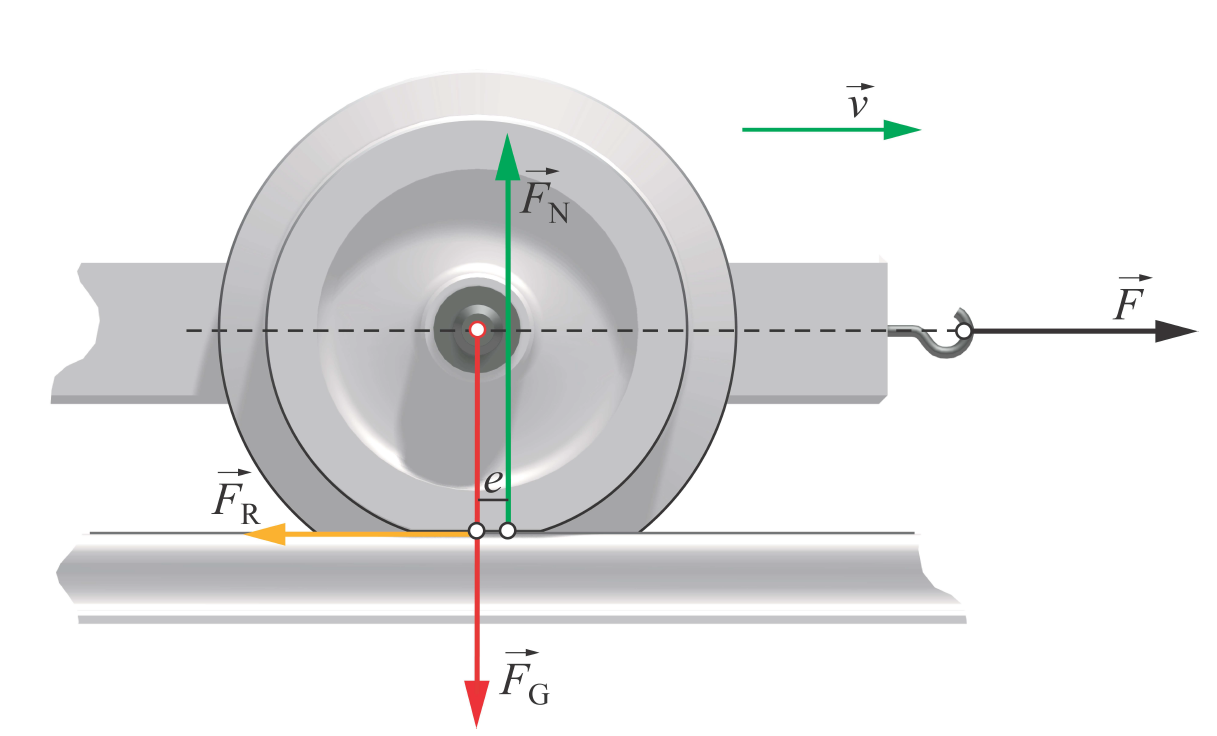
\includegraphics[width=0.8\linewidth]{Bilder/rollreibung_1} \\
		\end{minipage}
		\hfill
		\begin{minipage}{0.48\linewidth}
			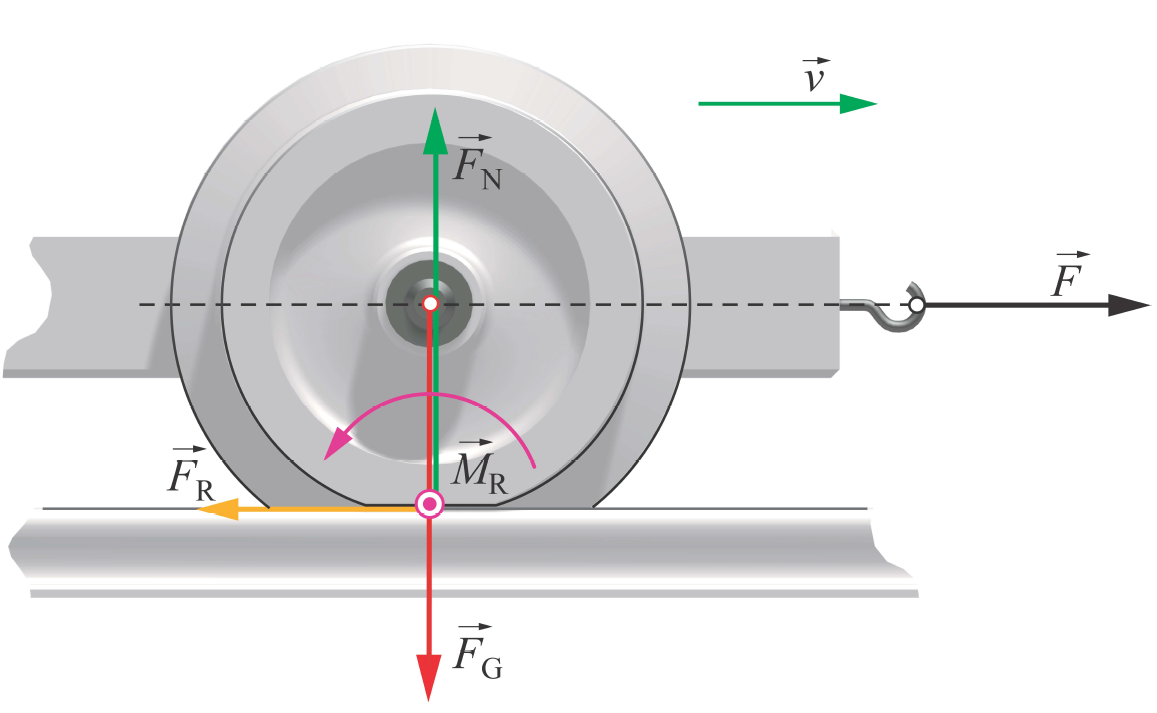
\includegraphics[width=0.8\linewidth]{Bilder/rollreibung_2} \\
		\end{minipage}
		
		$$ \boxed{ e = \frac{r \cdot F}{F_N} = \frac{r \cdot F_R}{F_N} =  \frac{r \cdot \mu_R \cdot F_R}{F_N} = \mu_R \cdot r }$$ 
		
		$$ \boxed{ M_R = e \cdot F_N = \mu_R \cdot r \cdot F_N = r \cdot F_R = r \cdot F} $$ \\

		\begin{tabular}{c l c}
			$e$ & Rollreibungslänge & $[e] = \mathrm{m}$ \\
			$r$ & Radius des Rades & $[r] = \mathrm{m}$ \\
			$F_R$ & Rollreibungskraft & $[F_R] = \mathrm{N}$ \\
			$F_N$ & Normalkraft & $[F_N] = \mathrm{N}$ \\
			$\mu_R$ & Rollreibungskoeffizient & $[\mu_R] = 1$ \\
			$M_R$ & Rollreibungsmoment & $[M_R] = \mathrm{Nm}$ \\
		\end{tabular}

	\subsection{Angetriebenes Rad}
	
		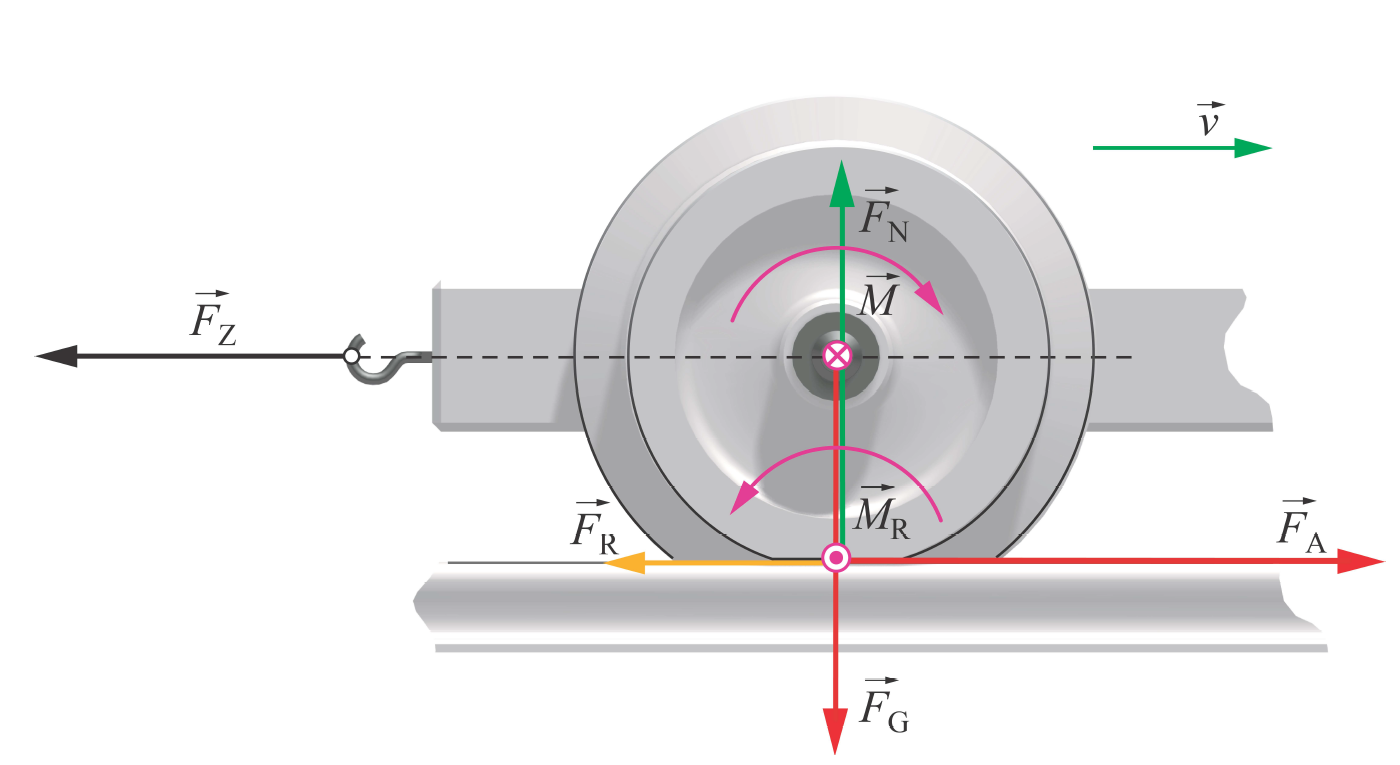
\includegraphics[width=0.8\linewidth]{Bilder/antriebsrad} \\
		\\

		\begin{tabular}{c l c}
			$\vec{F_Z}$ & Zugkraft & $[F_Z] = \mathrm{N}$ \\
			$\vec{F_N}$ & Normalkraft & $[F_N] = \mathrm{N}$ \\
			$\vec{F_R}$ & Rollreibungskraft & $[F_R] = \mathrm{N}$ \\
			$\vec{F_A}$ & Haftreibungskraft & $[F_A] = \mathrm{N}$ \\
		\end{tabular}

		\subsubsection{Hinweise zu Reibung an Rädern}
		
			\begin{tabular}{ll}
				$\bullet$ & Jedes Rad weist Rollreibung auf \\
				$\bullet$ & Zusätzlich zur Rollreibung weist ein angetriebenes Rad \\
				          & eine Haftreibung auf \\
			\end{tabular}

	\subsection{Arbeit und Energie}
	
		\subsubsection{Arbeit}
		
			Wird der Angriffspunkt einer Kraft $\vec{F}$ um die Strecke $d \vec{s}$ verschoben so leistet die Kraft die Arbeit $W$ 
			
			$$ \boxed{ W_{AB} =  \int \limits_A^B d \, W =  \int \limits_A^B \vec{F} \bullet d \, \vec{s} \qquad \text{(Skalarprodukt)} }$$ \\
			
			Wenn die projizierte Kraft konstant ist: $\boxed{ W = F \bullet s_{AB} }$ \\
			\\
			\begin{tabular}{c l c}
				$W$ & Arbeit & $[W] = \mathrm{N \cdot m = J}$ \\
				$F$ & Kraft & $[F] = \mathrm{N}$ \\
				$s$ & Weg & $[s] = \mathrm{m}$ \\
			\end{tabular}

		\subsubsection{Potentielle Energie $W_{pot}$}
			Beim Anheben eines Körpers gewinnt der Körper an potentieller Energie (Lageenergie) 
			
			$$ \boxed{ W_{pot} = m \cdot g \cdot h}$$
			\\
			\begin{tabular}{c l c}
				$W_{pot}$ & Potentielle Energie & $[W] = \mathrm{N \cdot m = J}$ \\
				$m$ & Masse des Körpers & $[m] = \mathrm{kg}$ \\
				$g$ & Erdbeschleunigung & $[g] = \mathrm{\frac{m}{s^2}}$ \\
				$h$ & Höhe der Körpers & $[h] = \mathrm{m}$ \\
				\\
			\end{tabular}
			
			\textbf{Beispiel: Spannen einer Feder} \\
				\\  
				Federkraft als Funktion der Auslenkung x \qquad $F = -k \cdot x$ \\
				\\
				$$ \boxed{ W_{pot} = \int \limits_0^{x_0}  - \vec{F} \bullet d \vec{x} = \int \limits_0^{x_0}  k \cdot x \, dx = \frac{1}{2} \, k \cdot \Delta x^2} $$ \\
				
			\begin{tabular}{c l c}
				$W_{pot}$ & Potentielle Energie & $[W] = \mathrm{N \cdot m = J}$ \\
				$F$ & Federkraft & $[F] = \mathrm{N} $ \\
				$k$ & Federkonstante & $[k] = \mathrm{\frac{N}{m}}$ \\
				$\Delta x$ & Auslenkung der Feder & $[\Delta x] = \mathrm{m}$ \\
			\end{tabular}

			\vfill\null
			\columnbreak

		\subsubsection{Kinetische Energie $W_{kin}$}
		
			$$ \boxed{ \normalsize{ W_{kin} = \int \limits_A^B \vec{F} \bullet d \, \vec{s} =  F \bullet s_{AB} = m \, a \cdot \frac{a}{2} t^2 = m \frac{a^2 \cdot t^2}{2} = \frac{1}{2} m \cdot v^2} }$$
			
			\begin{tabular}{c l c}
				$W_{kin}$ & Kinetische Energie & $[W] = \mathrm{N \cdot m = J}$ \\
				$F$ & Kraft & $[F] = \mathrm{N} $ \\
				$s$ & Wegstück (Kinematik) & $[s] = \mathrm{m}$ \\
				$m$ & Masse des Körpers & $[m] = \mathrm{kg}$ \\
				$a$ & Beschleunigung (Kinematik) & $[a] = \mathrm{\frac{m}{s^2}}$ \\
				$v$ & Geschwindigkeit (Kinematik) & $[v] = \mathrm{\frac{m}{s}}$ \\
			\end{tabular}

	\subsection{Energieerhaltung (in abgeschlossenen Systemen)}
	
		Die Gesamtenergie eines \underline{abgeschlossenen Systems} ist unveränderlich! \\
		\\
		\textbf{abgeschlossen: Es wird keine Masse hinzugefügt/entfernt und es wirken keine äusseren Kräfte!} \\
			\\	
			$$ \boxed{ W = \underbrace{m \cdot g \cdot h}_{\substack{\text{pot. Energie}}} =  m \cdot g \cdot \underbrace{ \frac{1}{2} \, g \cdot t^2}_{\substack{\text{h(t)}}}  = \underbrace{ \frac{1}{2} m \cdot v^2 }_{\substack{\text{kin. Energie}}} } $$ \\
			\\
			Für \underline{nicht abgeschlossene Systeme} kann eine Bilanzrechnung aufgestellt werden: \\
			Die Energiezunahme im Gesamtsystem entspricht der von aussen zugeführten Energie. \\
			Die Energieabnahme im Gesamtsystem entspricht der von aussen entzogenen Energie. \\

		\subsubsection{Energiesatz der Mechanik} 
			$$ \boxed{ E_{pot} + E_{kin} = E_{tot} = \text{const} } \qquad \text{(gilt zu jedem Zeitpunkt)} $$

	\subsection{Leistung und Wirkungsgrad}
	
		\subsubsection{Leistung}
		
			$$ \boxed{ P = \frac{\Delta W}{\Delta t} = \frac{\vec{F} \bullet \Delta \vec{s}}{\Delta t} = \vec{F} \frac{\Delta \vec{s}}{\Delta t} = \vec{F} \bullet \vec{v} } $$ 
			
			
			\begin{tabular}{c l c}
				$P$ & Leistung & $[P] = \mathrm{W = \frac{J}{s}}$ \\
				$\Delta W$ & geleistete Arbeit & $[W] = \mathrm{J}$ \\
				$\Delta t$ & verstrichene Zeit & $[t] = \mathrm{s}$ \\
				$F$ & Kraft & $[F] = \mathrm{N}$ \\
				$\Delta s$ & Wegstück & $[s] = \mathrm{m}$ \\
				\\
			\end{tabular}
			
			\textbf{Pferdestärken} \\
				\\
				$1 \; \mathrm{PS} = 75 \, \mathrm{kg} \cdot 9.81 \mathrm{\frac{m}{s^2}} \cdot 1 \mathrm{\frac{m}{s}} = 735.5 \, \mathrm{W}$ \\

		\subsubsection{Wirkungsgrad $\eta$}	
			Faustregel: Je grösser eine Maschine, desto besser ihr Wirkungsgrad \\
			
			$$ \boxed{ \eta = \frac{P_{ab}}{P_{zu}} } \qquad \textcolor{red}{\eta < 1} \qquad [\eta] = 1 $$

	\subsection{Impuls $\vec{p}$}
	
		$$ \boxed{ \vec{p} = m \cdot \vec{v} }$$ 
		
		2. Newton'sches Gesetz allgemeingültiger (relativistisch): \\
		
		$$ \boxed{ \vec{F} = m \cdot \vec{a} = m \cdot \frac{d \, \vec{v}}{dt} = \frac{d}{dt} (m \cdot \vec{v}) = \frac{d \, \vec{p}}{dt} } $$ 
		
		\begin{tabular}{c l c}
			$\vec{p}$ & Impuls & $[\vec{p}] = \mathrm{\frac{kg  \, m}{s}}$ \\
			$m$       & Masse & $[m] = \mathrm{kg}$ \\
			$\vec{v}$ & Geschwindigkeit & $[v] = \mathrm{\frac{m}{s}}$ \\
			$F$       & Kraft & $[F] = \mathrm{N}$ \\
			$\vec{a}$ & Beschleunigung & $[\vec{a}] = \mathrm{\frac{m}{s^2}}$ \\
		\end{tabular}

		\subsubsection{Kraftstoss $\Delta p$}
			Ein Kraftstoss entspricht einer Impulsänderung und kann über die mittlere Kraft beschrieben werden. \\
			\\
			\begin{minipage}{0.55\linewidth}
				$$ \boxed{ \int \limits_{t_a}^{t_a + \Delta t}  F(t) \, dt = \overline{F} \cdot \Delta t = \Delta p = p' - p } $$ 	
			\end{minipage}
			\hfill
			\begin{minipage}{0.42\linewidth}
				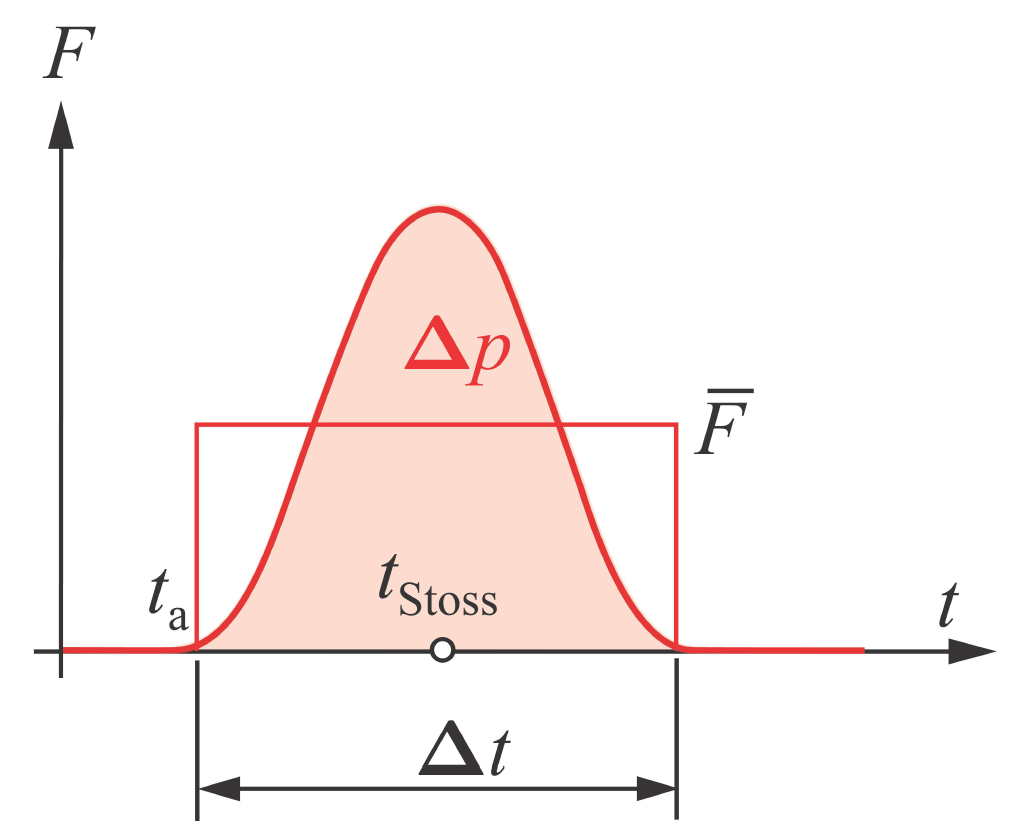
\includegraphics[width=0.8\linewidth]{Bilder/impuls} \\
			\end{minipage}
			
			\begin{tabular}{c l c}
				$F(t)$ & Kraftverlauf & $[F] = \mathrm{N}$ \\
				$\overline{F}$ & mittlere Kraft & $[\overline{F}] = \mathrm{N}$ \\
				$\Delta t$ & Zeitdauer des Kraftstosses & $[\Delta t] = \mathrm{s}$ \\
				$\Delta p$ & Impulsänderung & $[\Delta p] = \mathrm{Ns}$ \\
				$p$ & Impuls vor dem Stoss & $[p] = \mathrm{Ns}$ \\
				$p'$ & Impuls nach dem Stoss & $[p'] = \mathrm{Ns}$ \\
				$\vec{a}$ & Beschleunigung & $[\vec{a}] = \mathrm{\frac{m}{s^2}}$ \\
			\end{tabular}

	\subsection{Impulserhaltungssatz (Impulssatz)}
		In einem \textbf{abgschlossenen System} bleibt der Gesamtimpuls \\
		konstant \\
		abgeschlossenes System: es wirken keine externen Kräfte \\
		
		$$ \boxed{ \vec{p} =  \int \underbrace{  \frac{d \, \vec{p}}{dt} }_{\substack{F_{aussen} = 0}}   \, dt = c = \text{const} }  $$

	\subsection{Stösse}
	
		\begin{tabular}{ll}
			Elastizitätszahl: & $k = \frac{v_2' - v_1'}{v_1 - v_2} = - \frac{v'_{rel}}{v_{rel}} \geq 0$ \\
			\\
			Deformtionsarbeit: & $Q = (E_1 + E_2) - (E_1' + E_2') \geq 0$  \\
			\\
		\end{tabular}

		\begin{tikzpicture}
			[
			x=1cm, y=1cm, scale=0.5, font=\footnotesize, >=latex 
			%Voreinstellung für Pfeilspitzen
			]
			%Raster im Hintergrund
			%\draw[step=1, gray, very thin] (0,0) grid (5.5,5.5);
			
			%m1
			\begin{scope}[xshift=0cm, yshift=0cm, rotate=0, scale=1]
				%Kräfte
				\fill[gray!50!white] (0, 0) circle(1.25);
				\draw[thick] (0, 0) circle(1.25);
				\fill[black] (0, 0) circle(5pt) node [midway, above, yshift=2pt, scale=1.5] {$m_1$};
				\draw [-latex, very thick, purple] (1.25,0) -- ++(1.5,0) node[midway, above, scale=1.5] {$\vec{v}_1$};
			\end{scope}		
			
			%m2
			\begin{scope}[xshift=4cm, yshift=0cm, rotate=0, scale=1]
				%Kräfte
				\fill[gray!50!white] (0, 0) circle(0.75);
				\draw[thick] (0, 0) circle(0.75);
				\fill[black] (0, 0) circle(5pt) node [midway, above, yshift=2pt, scale=1.5] {$m_2$};
				\draw [-latex, very thick, purple] (0.75,0) -- ++(1.5,0) node[midway, above, scale=1.5] {$\vec{v}_2$};
			\end{scope}	
		\end{tikzpicture}

		\subsubsection{Gerader, zentraler, total elastischer Stoss}
			Die beiden Stosspartner verformen sich nicht!\\
			$\Rightarrow$ Für die Deformationsarbeit gilt: $Q = 0$ \\
			\boxed{
				\begin{tabular}{ll}
					Impulssatz: &  $p  \overset{!}{=} p'$ \\
					& $m_1 \, v_1 + m_2 \, v_2 \overset{!}{=} m_1 \, v_1' + m_2 \, v_2'$ \\
					\\
					Energiesatz: & $E_{kin} \overset{!}{=} E_{kin}'$ \\
					& $\frac{1}{2} m_1 \, v_1^2 + \frac{1}{2} m_2 \, v_2^2 \overset{!}{=} \frac{1}{2} m_1 \, v_1'^2 + \frac{1}{2} m_2 \, v_2'^2 $ \\
					\\
					& $v_1' = \frac{m_1 - m_2}{m_1 + m_2} \cdot v_1 + \frac{2 \, m}{m_1 + m_2} \cdot v_2$ \\
					\\
					& $v_2' = \frac{2 \, m_1}{m_1 + m_2} \cdot v_1 + \frac{m_2 - m_1}{m_1 + m_2} \cdot v_2$ \\
				\end{tabular}
			}

		\subsubsection{Gerader, zentraler, total inelastischer Stoss}
			Die beiden Stosspartner haften nach dem Stoss aneinander und haben die gleiche Geschwindigkeit. \\
			$\Rightarrow$ Für die Deformationsarbeit gilt: $Q \neq 0$ \\
			\boxed{
				\begin{tabular}{ll}
					Impulssatz: & $p  \overset{!}{=} p'$ \\
					& $m_1 \, v_1 + m_2 \, v_2 \overset{!}{=} (m_1 + m_2) \, v'$ \\
					\\
					Energiesatz: & $E_{kin} \overset{!}{=} E_{kin}'$ \\
					& $\frac{1}{2} m_1 \, v_1^2 + \frac{1}{2} m_2 \, v_2^2 \overset{!}{=} \frac{1}{2} (m_1 + m_2) \, v'^2 + Q$ \\
					\\
					Deformationsarbeit: & $Q = \frac{m_1 \, m_2}{2 (m_1 + m_2)} (v_1 - v_2)^2 =  \frac{1}{2} \mu \cdot v_{rel}^2 $ \\
					\\
					Relativgeschw.: & $v_{rel} := \vert v_1 - v_2  \vert$ \\
					\\
					Reduzierte Masse: & $\mu = \frac{m_1 \, m_2}{m_1 + m_2}$\\
				\end{tabular}
			}

			\begin{tabular}{c l c}
				$k$ & Elastizitätszahl & $[k] = 1$ \\
				$E_1, \,E_2$ & Energien vor Stoss & $[E] = \mathrm{J}$ \\	
				$E_1 ', \, E_2 '$ & Energien nach Stoss & $[E'] = \mathrm{J}$ \\	
				$m_1, \, m_2$ & stossende Massen & $[m] = \mathrm{kg}$ \\
				$v_1, \, v_2$ & Geschwindigkeit vor Stoss & $[v] = \mathrm{\frac{m}{s}}$ \\
				$v_1', \, v_2'$ & Geschwindigkeit nach Stoss & $[v'] = \mathrm{\frac{m}{s}}$ \\
				$Q$ & Deformationsarbeit & $[Q] = \mathrm{J}$ \\
				$v_{rel}$ & Relativgeschwindigkeit &  $[v_{rel}] = \mathrm{\frac{m}{s}}$ \\
				$\mu$ & reduzierte Masse & $[\mu] = \mathrm{kg}$ \\
			\end{tabular}

	\subsection{Rakete}
		\subsubsection{Rakete im Flug}
			$\Rightarrow$ Masse ist hier veränderbar! \qquad $m(t) = m = m_{Start} - \mu \cdot t$ \\
			\\
			Die Rakete verliert an Treibstoff, wodurch die Masse der Rakete abnimmt ($dm < 0$)\\
			\\	
			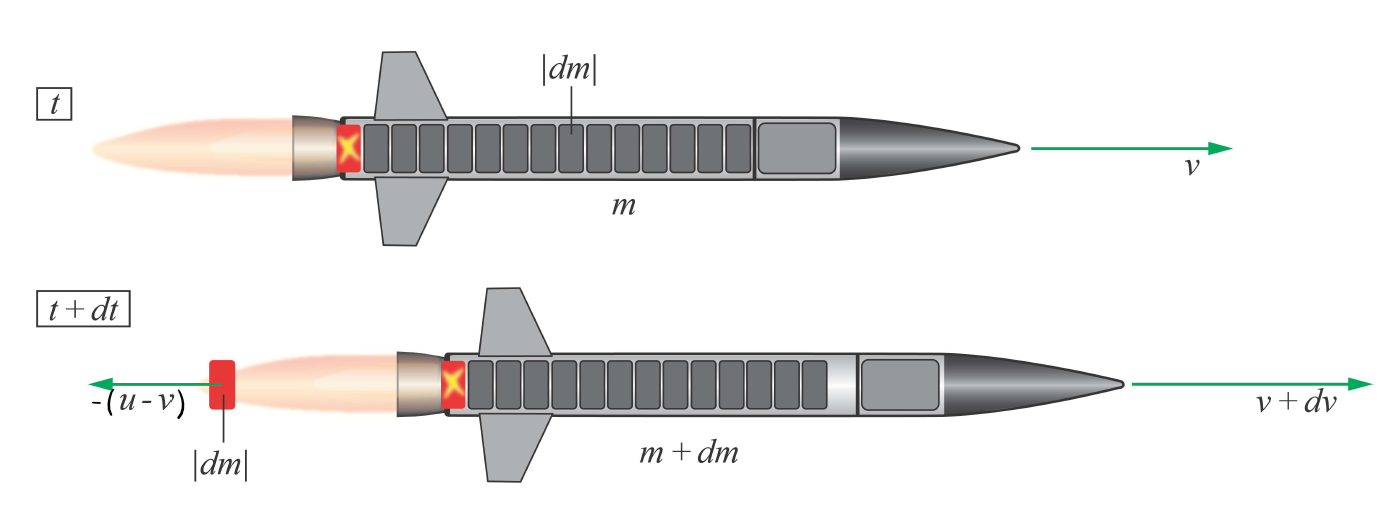
\includegraphics[width=0.73\linewidth]{Bilder/rakete} \\
			\\
			Impulssatz: \quad $ m \cdot v(t) = (m + dm)(v(t) + dv) + dm \,(u-v) $ \qquad $dm < 0$ \\
			\\
			Raketengleichung: $v(t) = - u \cdot \ln(m) + v_0 + u \cdot \ln(m_0) = v_0 + u \cdot \ln(\frac{m_0}{m})$ \\
			\\
			Massenverhältnis: $\frac{Startmasse}{Endmasse}$ \\
			\\
			max. Geschwindigkeitsänderung: $\Delta v = v - v_0 = u \cdot \ln(\frac{m_0}{m})$ \\
			\\
			Schubkraft: $F_{Schub} = \frac{dp}{dt} = - \frac{u \cdot dm}{dt} =  \underbrace{ \frac{dm}{dt} }_{\substack{\mu}} (-u) = \mu \cdot u$ \\ 
			\\
			$\Rightarrow$ Hier wurde noch keine Erdbeschleunigung (Anziehung) berücksichtigt! \\
			\\
			\\
			\begin{tabular}{c l c}
				$u$ &  Strahlgeschwindigkeit der Rakete & $[u] =  \mathrm{\frac{m}{s}}$ \\	
				$m$ & Zeitlich veränderbare Masse $m(t)$ & $[m] = \mathrm{kg}$ \\
				$m_0$ & Masse zum Startzeitpunkt & $[m] = \mathrm{kg}$ \\
				$v_0$ & Startgeschwindigkeit & $[v_0] = \mathrm{\frac{m}{s}}$ \\
				$F_{Schub}$ & Schubkraft der Rakete & $[F_{Schub}] = \mathrm{N}$ \\
				$\mu$ & Treibstoffverbrauch pro Zeit & $[\mu] = \mathrm{\frac{kg}{s}}$
			\end{tabular}

		\subsubsection{Aufstieg der Rakete im Schwerefeld}
			Konstante Erdbeschleunigung g wird berücksichtigt \\
			\\
			Veränderbare Masse: $m(t) = m = m_{Start} - \mu \cdot t$ \\
			\\
			Gesamtkraft: $m(t) \frac{dv}{dt} = m(t) \cdot a = F_{Schub} - F_G = \mu \cdot u - m \cdot g$ \\
			\\
			Beschleunigung: $a(t) = \frac{dv}{dt} = \frac{\mu \cdot u}{m_0 - \mu \cdot t} - g$ \\
			\\
			Raketengleichung: $v(t) = u \cdot \ln( \frac{m_{Start}}{m(t)} ) -  g \cdot t  $ \\
			\\
			Spezifischer Impuls: $T = \frac{m(t)}{\mu} = \frac{u}{g}$ \\
			\\
			Steighöhe: $h_t = u \cdot t - \frac{1}{2}gt^2 - \frac{u}{\mu} \cdot ln(\frac{m_0}{m_t}) \cdot m_t $
			\\
			\begin{tabular}{c l c}
				$u$ &  Strahlgeschwindigkeit der Rakete & $[u] =  \mathrm{\frac{m}{s}}$ \\	
				$m$ & Zeitlich veränderbare Masse $m(t)$ & $[m] = \mathrm{kg}$ \\
				$m_0$ & Masse zum Startzeitpunkt & $[m] = \mathrm{kg}$ \\
				$v_0$ & Startgeschwindigkeit & $[v_0] = \mathrm{\frac{m}{s}}$ \\
				$g$ & Erdbeschleuigung & $[g] = \mathrm{\frac{m}{s^2}}$ \\
				$\mu$ & Treibstoffverbrauch pro Zeit & $[\mu] = \mathrm{\frac{kg}{s}}$ \\
				$T$ & spezifischer Impuls (Zeit von konstantem Schub) & $[T] = \mathrm{s}$  \\
			\end{tabular}

	\subsection{Gravitation}
		\subsubsection{Erstes Kepler'sches Gesetz}
			Die Planeten bewegen sich auf Ellipsen, in deren Brennpunkt sich die Sonne befindet. \\
			\\
			\begin{minipage}{0.45\linewidth}
				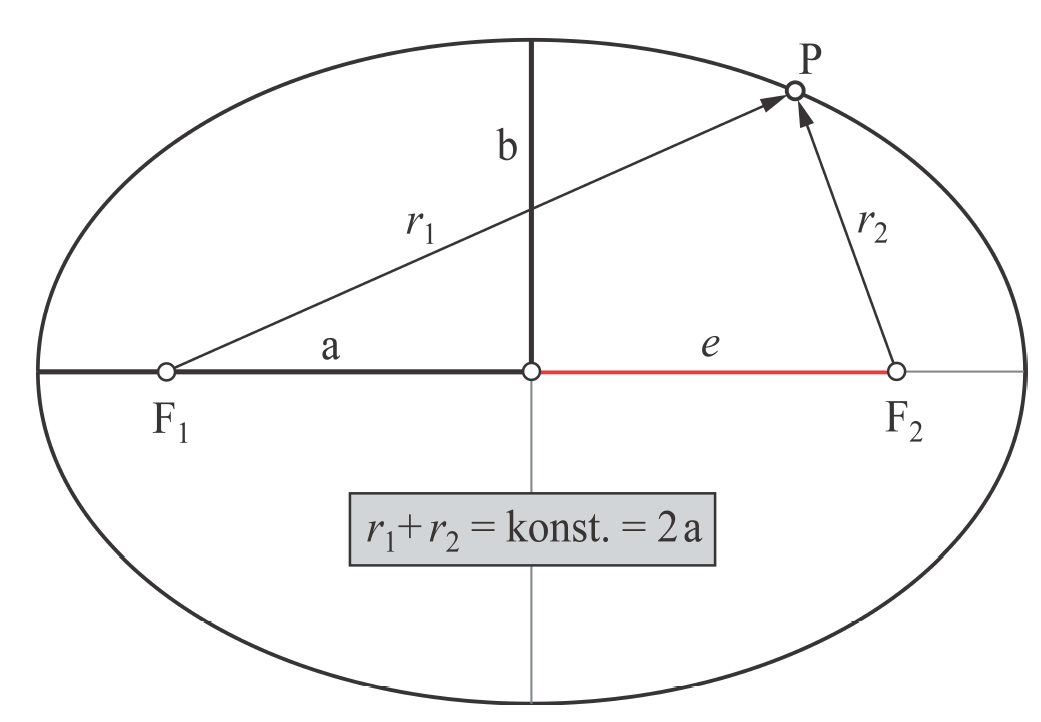
\includegraphics[width=\linewidth]{Bilder/ellipse}
			\end{minipage}
			\hfill
			\begin{minipage}{0.53\linewidth}
				\begin{tabular}{ll}
					$a$ & grosse Halbachse \\
					$b$ & kleine Halbachse \\
					$F_1, F_2$ & Brennpunkte \\
					$e$ & Exzentrizität \\
					$\epsilon$ & num. Exzentrizität $\epsilon = \frac{e}{a} $\\	
					$r_{min}$ & minimaler Radius \\	
					& $r_{min} = a \,(1 - \epsilon)$ \\
					$r_{max}$ & maximaler Radius \\
					& $r_{max} = a \,(1 + \epsilon)$ \\
				\end{tabular}
			\end{minipage}

		\subsubsection{Zweites Kepler'sches Gesetz}
			Der Fahrstrahl der Planeten überstreicht in der gleichen Zeit die gleiche Fläche. \\
			$\Rightarrow$ Bei kleinerem Abstand zur Sonne ist die Geschwindigeit schneller! \\
		
		\subsubsection{Drittes Kepler'sches Gesetz}
			Die Quadrate der Umlaufzeiten verhalten sich wie die Kuben der grossen Halbachsen. \\
			\\
			$a = \big(  \frac{T}{T_{ref}}^{\frac{2}{3}} \cdot a_{ref} \big)$ \qquad $\Leftrightarrow$ \qquad $\big( \frac{a}{a_{ref}}  \big)^3 =  \big( \frac{T}{T_ref}  \big)^2 $ \\
			\\
			Als Referenz wird die Erde verwendet! \\
			\\
			Astronomische Einheit: $a_{ref} = 1 \, \mathrm{AE} = 149.6 \cdot 10^6 \, \mathrm{km}$ \\
			\\
			Referenzzeit: $T_{ref} = 1 \, a = 1 \; \mathrm{Jahr}$ \\
			\\
			\begin{tabular}{c l c}
				$a$ & grosse Halbachse gesuchtet Planet & $[a] = \mathrm{AE}$ \\
				$a_{ref}$ &  grosse Halbachse Erde & $[a_{ref}] = \mathrm{AE}$ \\	
				$T$ & Umlaufzeit Planet & $[T] = \mathrm{Jahre}$ \\
				$T_{ref}$ & Umlaufzeit Erde & $[T] = \mathrm{Jahre}$ \\
			\end{tabular}

		\subsubsection{Gravitationsgesetz}
		
			$$ \boxed{ \text{Gravitationskraft:}  \quad F_G = G \, \frac{m_1 \cdot m_2}{r^2} \quad \text{mit }G = 6.67 \cdot 10^{-11} \mathrm{\frac{m^3}{kg \, s^2}} }$$ 

		\subsubsection{Gravitationswirkung innerhalb einer Kugel}
		
			$$ \boxed{ F_G = G \, \frac{m_{Kern} (r) \, m}{r^2} =  G \, \frac{4 \, \pi \, r^3 \, \rho \, m}{3 \, r^2} = \frac{4 \, \pi}{3} \, G \, \rho \, m \, r } $$ \\
		
			\begin{tabular}{c l c}
				$F_G$ & Gravitationskraft & $[F_G] = \mathrm{N}$ \\
				$G$ & Gravitationskonstante & $[G] = \mathrm{\frac{m^3}{kg \, s^2}}$ \\	
				$r$ & Radius (Abstand vom Zentrum) & $[r] = \mathrm{m}$ \\
				$\rho$ & homogene Dichte der Kugel & $[\rho] = \mathrm{\frac{kg}{m^3}}$ \\
				$m$ & Masse vom Massepunkt & $[m] = \mathrm{kg}$ \\
				$m_{Kern}$ & Masse des Kugelkerns & $[m_{Kern}] = \mathrm{kg}$ \\
			\end{tabular}

		\subsubsection{Gravitationswirkung ausserhalb einer Kugel}
		
			$$ \boxed{ F_G = G \, \frac{M \cdot m}{r^2}}  $$ \\
			
			\begin{tabular}{c l c}
				$F_G$ & Gravitationskraft & $[F_G] = \mathrm{N}$ \\
				$G$ & Gravitationskonstante & $[G] = \mathrm{\frac{m^3}{kg \, s^2}}$ \\	
				$r$ & Radius (Abstand vom Zentrum) & $[r] = \mathrm{m}$ \\
				$m$ & Masse vom Massepunkt & $[m] = \mathrm{kg}$ \\
				$M$ & Gesamtmasse der Kugel & $[M] = \mathrm{kg}$ \\
			\end{tabular}

		\subsubsection{Gravitationspotential  $\phi$}
		
			Wenn eine Masse in einem Gravitationsfeld bewegt wird, so wird Arbeit verrrichtet. \\
			\\
			$$ \boxed{ W_{12} = \int \limits_{r_1}^{r_2} \vec{F}_G \bullet d \vec{s}  =  \int \limits_{r_1}^{r_2} G \, \frac{M \cdot m}{r^2} \, dr = G \cdot M \cdot m \big( \frac{1}{r_2} - \frac{1}{r_1}  \big) }  $$  
			
			$$ \boxed{ \text{potentielle Energie:} \quad E_{pot}(r) = -G \, \frac{M \, m}{r} }$$ 
			
			$$ \boxed{ \text{Gravitationspotential:} \quad \phi = \frac{E_{pot}}{m} = - \frac{G \cdot M}{r}}  $$ \\

			\textbf{Im Inneren eines homogenen Zentralkörpers gilt} \\
			
				$$ \boxed{ F_G = \frac{4 \, \pi \cdot G \cdot \rho \cdot m \cdot r}{3} }$$ 
				
				$$ \boxed{ E_{pot} = - \frac{2 \,  \pi \cdot G \cdot \rho \cdot m}{3} \, r^2 + c' } $$
				
				$$ \boxed{ \phi = - \frac{2 \,  \pi \cdot G \cdot \rho}{3} \, r^2 + c = - \frac{G \cdot M(r)}{2 \, r}  + c = - \frac{G \cdot M(r)}{2 \, r} - \frac{G \cdot M}{2 \, R} } $$ \\
				
			\begin{tabular}{c l c}
				$W$ & Arbeit & $[W] = \mathrm{J} $ \\
				$F_G$ & Gravitationskraft & $[F_G] = \mathrm{N}$ \\
				$E_{pot}$ & potentielle Energie & $E_{pot} = \mathrm{J}$ \\
				$G$ & Gravitationskonstante & $[G] = \mathrm{\frac{m^3}{kg \, s^2}}$ \\	
				$r$ & Radius (Abstand vom Zentrum) & $[r] = \mathrm{m}$ \\
				$\rho$ & homogene Dichte der Kugel & $[\rho] = \mathrm{\frac{kg}{m^3}}$ \\
				$m$ & Masse vom Massepunnkt & $[m] = \mathrm{kg}$ \\
				$M$ & Gesamtmasse der Kugel & $[M] = \mathrm{kg}$ \\
				$R$ & Radius der Kugeloberfläche & $[R] = \mathrm{m}$ \\
			\end{tabular}

	\subsection{Bezugssysteme: Inertialsystem}
		Inertialsystem: \textbf{unbeschleuigtes} Bezugssystem \\
		\\
		Wenn die Newton'schen Gesetze im Bezugssystem S gelten, so gelten sie auch im Bezugssystem S', solange dieses nicht beschleunigt ist und nicht rotiert. \\
		$\Rightarrow$ \textbf{In sämtlichen Inertialsystemen sind die mechanischen Gesetze identisch!} \\

		\subsubsection{Galilei-Transformation}
			\begin{minipage}{0.48\linewidth}
				Bezugssystem S' bewegt sich mit konstanter Geschwindigkeit $v_0$: \\
				\\
				\\
				$v_0 = \begin{pmatrix}v_x \\ v_y \\ v_z\end{pmatrix}$
			\end{minipage}
			\hfill
			\begin{minipage}{0.42\linewidth}
				Transformation zwischen \\
				S und S' \\
				\\
				$x = x' + v_x t$ \\
				$y = y' + v_y t$ \\
				$z  = z' + v_z t$ \\
				$t = t'$
			\end{minipage}

	\subsection{Beschleunigte Bezugssysteme}
		In beschleunigten Bezugssystemen müssen \textbf{Trägheitskräfte} berücksichtigt werden!

		\subsubsection{Translatorisch beschleunigtes Bezugssystem}
			Beispiel: Zug beschleunigt auf gerader Schiene \\
			\\
			Für einen Beobachter \textbf{im beschleunigten System} S' wirkt \\
			eine Trägheitskraft: 
			
			$$ \boxed{ \text{Gesamtkraft:} \quad \vec{F}' = \vec{F} - m \cdot \vec{a}_0 = \vec{F} + \vec{F}_{Tr"agheit} }$$ \\
			
			\begin{tabular}{c l c}
				$\vec{F}'$ & Gesamte im System wirkende Kraft & $[\vec{F}'] = \mathrm{N}$ \\
				$\vec{F}$ & Statisch wirkende Kräfte & $[\vec{F}] = \mathrm{N}$ \\
				$\vec{F}_{Tr"agheit}$ & Trägheitskraft & $[\vec{F}_{Tr"agheit}] = \mathrm{N}$ \\
				$m$ & Masse im System & $[m] = \mathrm{kg}$ \\
				$\vec{a}_0$ & Beschleunigung des Systems & $[\vec{a}_0] = \mathrm{\frac{m}{s^2}}$ \\
			\end{tabular}

		\subsubsection{Gleichförmig rotierendes Bezugssystem (Scheinkräfte)}

			\textbf{Fest verbundene Masse} $\Rightarrow$ \textbf{Scheinkraft: Zentrifugalkraft} \\
				\\
				\begin{minipage}{0.48\linewidth}
					$$ \boxed{ \vec{F}_z = - m \, \vec{a}_z = - m \cdot \omega^2 \cdot \vec{r} }$$ 
					
					$$ \boxed{ \vec{F}_{Zentrifugal}  \overset{!}{=} - \vec{F}_{Zentripetal} }$$ 
				\end{minipage}
				\hfill
				\begin{minipage}{0.48\linewidth}
					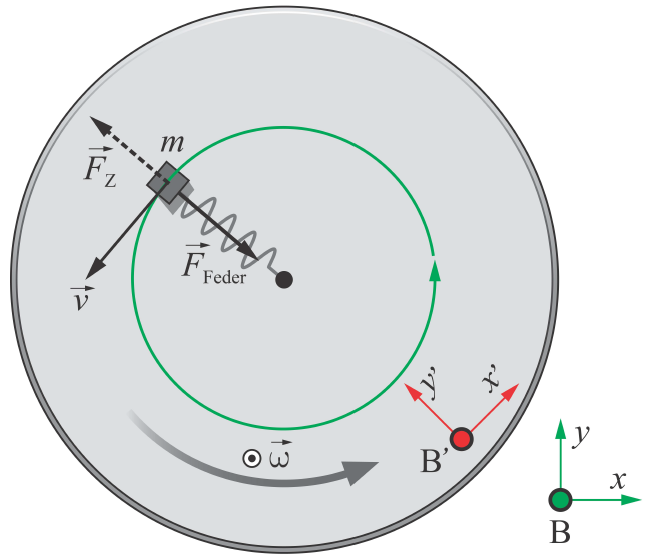
\includegraphics[width=0.75\linewidth]{Bilder/zentrifugalkraft} \\
				\end{minipage}
				\\
				\begin{tabular}{c l c}
					$\vec{F}_z$ & Zentrifugalkraft (Trägheitskraft; Scheinkraft) & $[\vec{F}_z] = \mathrm{N}$ \\
					$m$ & Masse im System & $[m] = \mathrm{kg}$ \\
					$\vec{a}_z$ & Beschleunigung des Systems ($a_{radial}$) & $[\vec{a}_z] = \mathrm{\frac{m}{s^2}}$ \\
					$\omega$ & Winkelgeschwindigkeit & $[\omega] = \mathrm{\frac{rad}{s}}$ \\
					$\vec{r}$ & Radius des Systems (nach innen zeigend) & $[\vec{r}] = \mathrm{m}$ \\ 
					\\
					\\
				\end{tabular}

			\textbf{lose Masse} $\Rightarrow$ \textbf{Scheinkraft: Corioliskraft} \\	
				\\
				\\
				\begin{minipage}{0.48\linewidth}
					$$ \boxed{\vec{F}_c = - m \cdot \vec{a}_c = - m \cdot 2 \, (\vec{\omega} \times \vec{v}_R)} $$ 
				\end{minipage}
				\hfill
				\begin{minipage}{0.48\linewidth}
					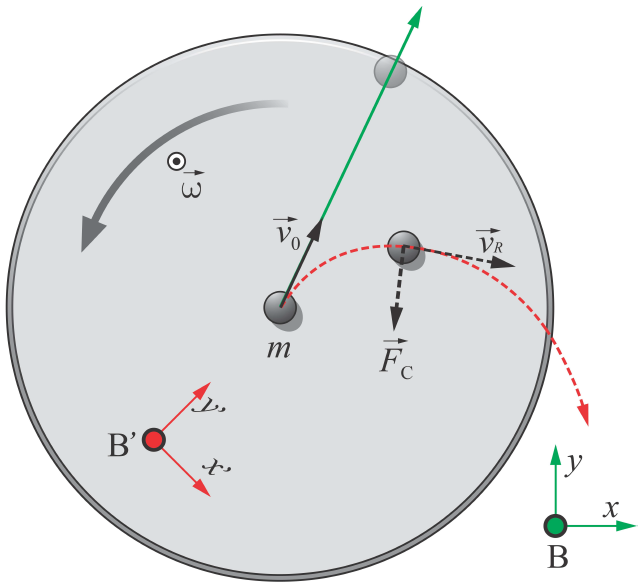
\includegraphics[width=0.75\linewidth]{Bilder/corioliskraft} \\
				\end{minipage}
				\\
				\begin{tabular}{c l c}
					$\vec{F}_c$ & Corioliskraft (Trägheitskraft; Scheinkraft) & $[\vec{F}_c] = \mathrm{N}$ \\
					$m$ & Masse im System & $[m] = \mathrm{kg}$ \\
					$\vec{a}_c$ & Coriolisbeschleunigung & $[\vec{a}_c] = \mathrm{\frac{m}{s^2}}$ \\
					$\omega$ & Winkelgeschwindigkeit & $[\omega] = \mathrm{\frac{rad}{s}}$ \\
					$\vec{v}_R$ & Relativgeschwindigkeit & $[\vec{v}_R] = \mathrm{\frac{m}{s}}$ \\ 
				\end{tabular}

		\subsubsection{D'Alembert'sches Prinzip}
			Wird ein Körper in einem mitbewegten Koordinatensystem \\
			betrachtet, so bleibt er in Ruhe: \quad $\vec{v}_R = 0$ und $\vec{a}_R = 0$ \\
			
			$$ \boxed{ \vec{F} + \underbrace{ \vec{F}_z + \vec{F}_c }_{\substack{\text{Scheinkräfte}}} = \vec{0} }$$ 
			
			$\Rightarrow$ Statisches Gleichgewichtsproblem

	\subsection{Rotation starrer Körper}
	
		\begin{tabular}{ll}
			Rotation: & Drehung um feste Achse \\
			Kreisel: & Drehung um starren Punkt \\
			Kreiselbewegung & Drehung eines völlig freien, \\
			&  starren Körpers um seinen Schwerpunkt \\
		\end{tabular}

		\subsubsection{Dynamisches Grundgesetz der Rotation}
			Es ist \textbf{nur die tangentiale Komponente} der Kraft \\
			(des Drehmoments) eines rotierenden Körpers relevant! \\
				
			$$dM_t = r \cdot dF_t = r \cdot dm \cdot a_t = dm \cdot r^2 \cdot \alpha$$ \\
			
			$$ \boxed{ M = \int dM = \int r^2 \, \alpha \cdot dm = \alpha  \underbrace{  \int r^2 \cdot dm }_{\substack{J_{Scheibe} = m \cdot r^2}} }$$ \
			
			$$ \boxed{ \Rightarrow \; M = J \cdot \alpha = r \cdot F} $$ \\
				
			\begin{tabular}{c l c}
				$dM_t$ & kleine Tan.-Komponente des Drehmoments & $[dM_t] = \mathrm{Nm}$ \\
				$M$ & (gesamtes) Drehmoment & $[M] = \mathrm{Nm}$ \\
				$dF_t$ & kleine Tangentialkomponente der Kraft & $[dF_t] = \mathrm{N}$ \\
				$r$ & Abstand Drehachse zu Massepunkt (Rand) & $[r] = \mathrm{m}$ \\
				$dm$ & kleines Massestück des Körpers & $dm = \mathrm{kg}$ \\
				$a_t$ & Tangentialbeschleunigung ($a_t = r \cdot \alpha$) & $[a_t] = \mathrm{\frac{m}{s^2}}$ \\
				$\alpha$ & Winkelbescheunigung & $[\alpha] = \mathrm{\frac{rad}{s^2}}$ \\
				$J$ & (Massen-) Trägheitsmoment & $[J] = \mathrm{kg \, m^2}$ \\
			\end{tabular}

		\subsubsection{Massenträgheitsmomente} %TODO: Irgendwann mal Bilder gegen ganze Tabelle tauschen
		
			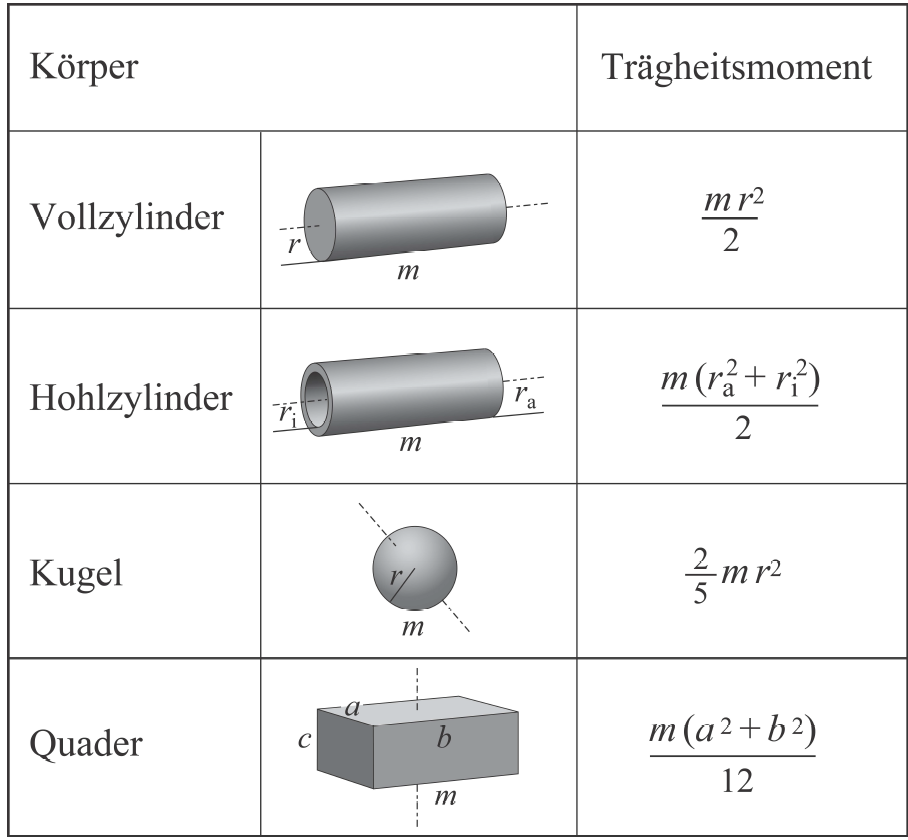
\includegraphics[width=0.8\linewidth]{Bilder/massentraegheitsmomente}

			Ring: $m \cdot r^2$

	\subsection{Trägheitsellipsoid}
		Trägheitsradius $r_0$: als ob ganze Masse eines Körpers nur einen \\
		Radius hätte \\
		\\
		\begin{minipage}{0.48\linewidth}
			$$ \boxed{ r_0 = \sqrt{\frac{J}{m}}} $$
		\end{minipage}
		\hfill
		\begin{minipage}{0.48\linewidth}
			$$ \boxed{s_0 = \frac{1}{r_0} }$$
		\end{minipage}
		
		\begin{tabular}{c l c}
			$r_0$ & Trägheitsradius & $[r_0] = \mathrm{m}$ \\
			$m$ & Masse des Körpers & $[m] = \mathrm{kg}$ \\
			$J$ & (Massen-) Trägheitsmoment & $[J] = \mathrm{kg \, m^2}$ \\
			$s_0$ & reziproker Trägheitsradius & $[s_0] = \mathrm{m}$ \\
			\\
		\end{tabular}
		
		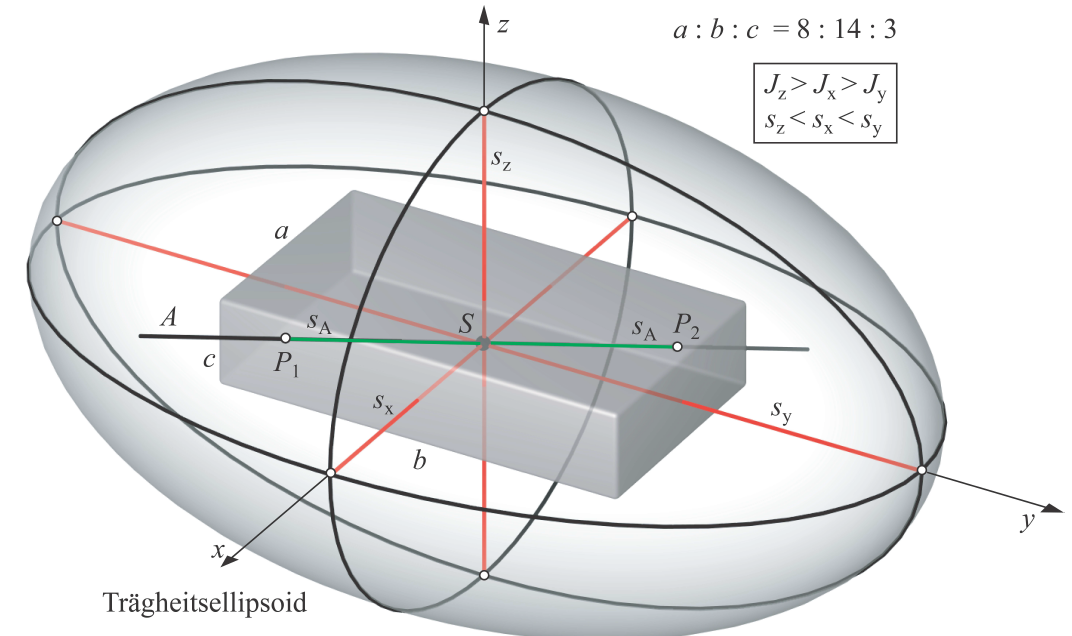
\includegraphics[width=0.8\linewidth]{Bilder/traegheits_ellipsoid} \\	
		\\
		\textcolor{red}{Hauptträgheits-Achsen} (entsprechen immer Symmetrie-Achsen, falls vorhanden) \\
		\textcolor{green}{beliebige Achse $J_A$} \quad $J_A = J_x \cdot \cos^2(\alpha) + J_y \cdot \cos^2(\beta) + J_z \cdot \cos^2(\gamma)$

	\subsection{Satz von Steiner}
		Beschreibt, wie man das Trägheitsmoment $J$ berechnet, wenn die Drehachse nicht durch den Schwerpunkt des rotierenden Körpers geht, sonden \textbf{parallel} dazu verläuft. \\
		
		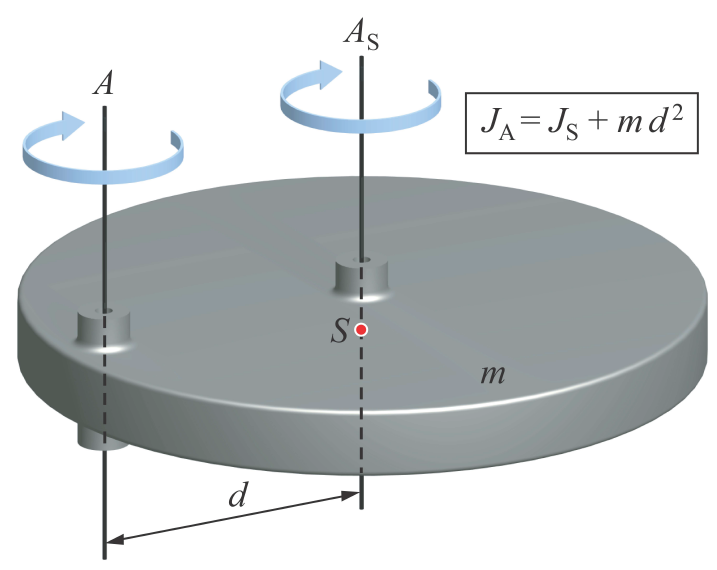
\includegraphics[width=0.6\linewidth]{Bilder/steiner} \\	
		\\
		\begin{tabular}{c l c}
			$J_S$ & Trägheitsmoment (Rot. um Schwerp.)  & $[J_S] = \mathrm{kg \, m^2}$ \\
			$J_A$ & Trägheitsmoment (Rot. um bel. Punkt)  & $[J_A] = \mathrm{kg \, m^2}$ \\
			$m$ & Masse des Körpers & $[m] = \mathrm{kg}$ \\
			$d$ & Abstand zum Schwerpunkt & $[d] = \mathrm{m}$ \\
		\end{tabular}

	\subsection{Arbeit und Leistung (Rotation)}
		$dW = \vec{F} \bullet d\vec{s} = F_t \cdot ds = F_t \cdot r \cdot d \phi = M \cdot d \phi $ \\
		\\
		$P = \frac{dW}{dt} = M \frac{d \phi}{dt} = M \cdot \omega$ \\
		\\
		\begin{tabular}{c l c}
			$F_t$ & \textbf{Tantentialer} Kraftanteil der Rotation & $[F_t] = N$ \\
			$d \phi$ & zurückgelegter Kreiswinkel & $[d \phi] = rad$ \\	
			$P$ & Leistung  & $[P] = W$ \\
			$W$ & Energie  & $[W] = J$ \\
			$\omega$ & Winkelgeschwindigkeit & $[\omega] = \frac{rad}{s}$ \\
			$M$ & Drehmoment & $[M] = Nm$ \\
		\end{tabular}

	\subsection{Rotationsenergie}
		\textbf{Folgendes gilt nur für die Rotation um den Schwerpunkt eines Körpers!} \\
		
		Die totale kinetische Energie ist die Summe aller kinetischer Energien eines Körpers \\
		
		$$ \boxed{ E_{kin} = \int \frac{1}{2} \, v^2 \, dm  = E_{trans} + E_{rot} } $$ 
		
		\begin{minipage}{0.48\linewidth}
			$$ \boxed{ E_{trans} = \frac{1}{2} \, m \cdot v_s^2 } $$ 
		\end{minipage}
		\hfill
		\begin{minipage}{0.48\linewidth}
			$$ \boxed{ E_{rot} = \frac{1}{2} \, J_s \cdot \omega^2 } $$ 
		\end{minipage}

		\begin{tabular}{c l c}
			$E_{trans}$ & Translationsenergie des Schwerpunkts & $[E_{trans}] = \mathrm{J}$ \\
			$m$ & Masse des Körpers & $[m] = \mathrm{kg}$ \\
			$v_s$ & Geschwindigkeit des Schwerpunkts & $[v_s] = \mathrm{\frac{m}{s}}$ \\
			$E_{rot}$ & Rotationsenergie & $[E_{rot}] = \mathrm{J}$ \\
			$J_S$ & Trägheitsmoment (Rot. um Schwerp.)  & $[J_S] = \mathrm{kg \, m^2}$ \\
			$\omega$ & Winkelgeschwindigkeit & $[\omega] = \mathrm{\frac{rad}{s}}$ \\
		\end{tabular}
	 
	\subsection{Drehimpuls $\vec{L}$ / Impulserhaltung (Rotation)}
		\begin{minipage}{0.42\linewidth}
			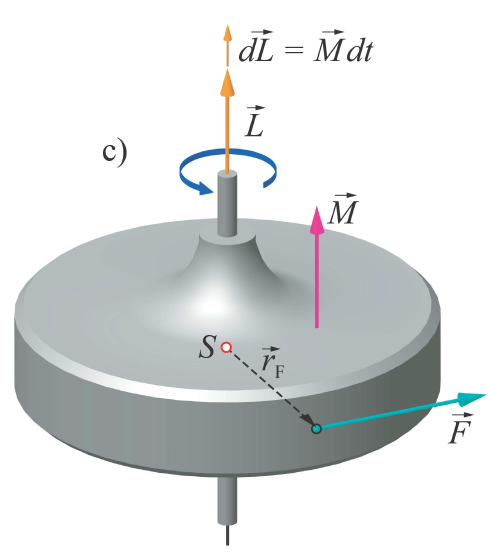
\includegraphics[width=\linewidth]{Bilder/drehimpuls} \\
			\\
		\end{minipage}
		\hfill
		\begin{minipage}{0.56\linewidth}
			$$ \boxed{ \vec{L} = \int d \vec{L} = \int \vec{r} \times \vec{v} \cdot dm = \vec{r} \times \vec{p} }$$ \\
		\end{minipage}

		\begin{tabular}{c l c}
			$\vec{L}$ & Drehimpuls & $[\vec{L}] = \mathrm{\frac{kg \, m^2}{s}}$ \\
			$\vec{r}$ & Abstand Massepunkt zu Rot-Achse & $[\vec{r}] = \mathrm{m}$ \\
			$\vec{v}$ & Rotationsgeschwindigkeit & $[\vec{v}] = \mathrm{\frac{m}{s}}$ \\
			$dm$ & kleines Masse-Stück & $[dm] = \mathrm{kg}$ \\
			$\vec{p}$ & Impuls & $[\vec{p}] = \mathrm{\frac{kg \, m}{s}}$ \\
		\end{tabular}

		\subsubsection{Energie beim Runterrollen}

			$$ \boxed{E_{pot} = E_{kin} + E_{rot} , \quad \quad m \cdot g \cdot h = \frac{1}{2}m \cdot v^2 + \frac{1}{2}J \cdot \omega^2} $$

		\subsubsection{Drehmoment $\vec{M}$ vs. Drehimpuls $\vec{L}$}
			$$ \boxed{ \vec{M} = \vec{r} \times \vec{F} = \frac{d}{dt} (\vec{r} \times \vec{p}) =  \frac{d}{dt} \vec{L} = \dot{\vec{L}} }$$ \\
			
			\textbf{In einem abgschlossenen System ($\vec{M} = 0$) bleibt der \\
			Gesamtdrehimpuls erhalten} \\
			$\Rightarrow \vec{L} = \text{const}$ \\
			\\
			\boxed{
				\begin{tabular}{ll}
					Impulserhaltung: &  $L  \overset{!}{=} L'$ \\
					& $J_1 \cdot \omega + J_2 \cdot \omega \overset{!}{=} J_1 \cdot \omega_1' + J_2 \cdot \omega_2'$ \\
					\\
					Energiesatz: & $E_{rot} \overset{!}{=} E_{rot}' + Q$ \\
					& $\frac{1}{2} J_1 \cdot \omega_1^2 + \frac{1}{2} J_2 \cdot \omega_2^2 \overset{!}{=} \frac{1}{2} J_1 \cdot \omega_1'^2 + \frac{1}{2} J_2 \cdot \omega_2'^2 + Q $ \\
				\end{tabular}
			}
			\\
			\\
			\begin{tabular}{c l c}
				$\vec{M}$ & Drehmoment & $[\vec{M}] = \mathrm{Nm}$ \\
				$\vec{r}$ & Abstand Massepunkt zu Rot-Achse & $[\vec{r}] = \mathrm{m}$ \\
				$\vec{F}$ & Kraft, welche Drehmoment bewirkt & $[\vec{F}] = \mathrm{N}$ \\
				$\vec{p}$ & Impuls & $[\vec{p}] = \mathrm{\frac{kg \, m}{s}}$ \\
				$\vec{L}$ & Drehimpuls & $[\vec{L}] = \mathrm{\frac{kg \, m^2}{s}}$ \\
				$J$  & Massenträgheitsmoment & $[J] = \mathrm{kg \, m^2}$ \\
				$\omega$ & Winkelgeschwindigkeit & $[\omega] = \mathrm{\frac{1}{s}}$ \\
				$Q$ & Deformationsarbeit & $[Q] = \mathrm{J}$ \\
			\end{tabular}

		\subsubsection{Drehimpuls $\vec{L}$ vs. Winkelgeschwindigkeit $\omega$}

		$$ \boxed{ L = \int dL = \int r^2 \, \omega \, dm = \omega \int r^2 \, dm = J \, \omega }$$ \\
		
			\begin{tabular}{c l c}
				$L$ & Drehimpuls & $[L] = \mathrm{\frac{kg \, m^2}{s}}$ \\
				$r$ & Abstand Massepunkt zu Rot-Achse & $[r] = \mathrm{m}$ \\
				$dm$ & kleines Masse-Stück & $[dm] = \mathrm{kg}$ \\
				$\omega$ & Winkelgeschwindigkeit & $[\omega] = \mathrm{\frac{rad}{s}}$ \\
				$J$ & (Massen-) Trägheitsmoment (hier Tensor) & $[J] = \mathrm{kg \, m^2}$ \\
			\end{tabular}

	\subsection{Rotation vs. Translation}
	
		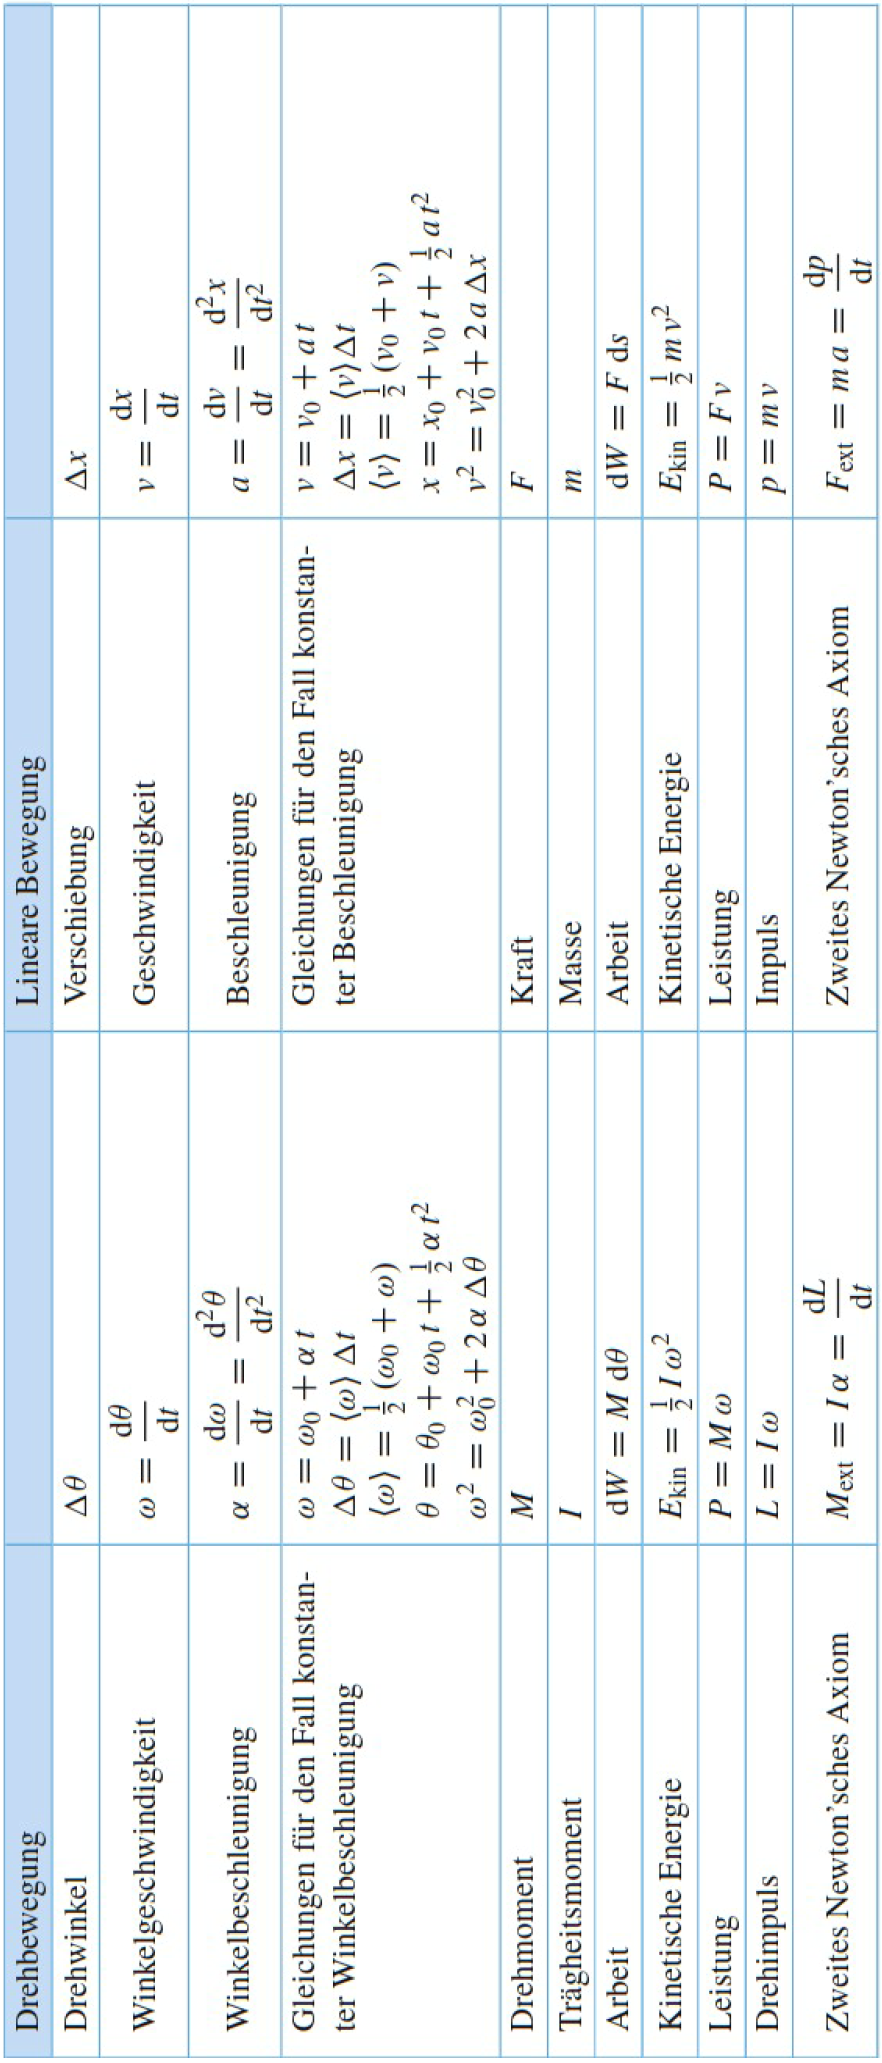
\includegraphics[width=0.85\linewidth]{Bilder/rotation_translation}
		
		% %Code geputzt, Inhalt kontrolliert

		\section{Hydrostatik}

\subsection{Festkörper, Flüssigkeit, Gas}

\subsubsection{Festkörper}

\begin{tabular}{ll}
	$\bullet$ & kein Fluid \\
	$\bullet$ & festes Volumen; feste Gestalt \\
	$\bullet$ & Moleküle / Atome befinden sich in regelmässiger \\
			  & Gitter-Anordnung \\
	$\bullet$ & inkompressibel (sehr schlecht komprimierbar) \\
	$\bullet$ & Kraft: Weiterleitung (längs ihrer Wirkungslinie) \\
	$\bullet$ & Druck: Verstärkung \\
\end{tabular}

\subsubsection{ideale Flüssigkeit}

\begin{tabular}{ll}
	$\bullet$ & Fluid \\
	$\bullet$ & festes Volumen; keine feste Gestalt \\
	$\bullet$ & Moleküle / Atome bewegen sich chaotisch aneinander vorbei \\
	$\bullet$ & Moleküle / Atome füllen den Raum aus / berühren sich \\
	$\bullet$ & inkompressibel (schlecht komprimierbar) \\
	$\bullet$ & reibungsfrei (keine Scherkräfte)\\
	$\bullet$ & Kraft: Verstärkung \\
	$\bullet$ & Druck: Weiterleitung (gleichmässig) \\
\end{tabular}



\subsubsection{Gas}

\begin{tabular}{ll}
	$\bullet$ & Fluid \\
	$\bullet$ & kein festes Volumen; keine feste Gestalt \\
	$\bullet$ & Moleküle / Atome fliegen mit hoher Geschwindigkeit durch\\
			  & den Raum \\
	$\bullet$ & Es gibt sehr viel Zwischenraum \\
	$\bullet$ &  Moleküle / Atome führen bei Zusammenstoss unter sich oder\\
			  & mit Gefässwand elestische Stösse aus \\
	$\bullet$ & kompressibel (gut komprimierbar)  \\
	$\bullet$ & reibungsfrei (keine Scherkräfte)\\

\end{tabular}


% \vfill\null
% \columnbreak


\subsection{Druck $p$ / Schubspannung $\tau$}
\textbf{Druck ist eine skalare Grösse (hat keine Richtung)} 


$$\boxed{ p = \frac{F_{\perp}}{A} } \qquad \boxed{ \tau = \frac{F_{\parallel}}{A} } $$

	\begin{tabular}{c l c}
		$p$ & Druck & $[p] = \mathrm{Pa = \frac{N}{m^2}}$ \\
		$\tau$ & Schubspannung (Scherkraft) & $[\tau] = \mathrm{N} $ \\
		$F_{\perp}$ & Kraft senkrecht zu A & $[F_{\perp}] = \mathrm{N}$ \\
		$F_{\parallel}$ & Kraft parallel zu A & $[F_{\parallel}] = \mathrm{N}$ \\
		$A$ & Fläche & $[A] = \mathrm{m^2}$ \\
		\\
	\end{tabular}
	
	\textbf{In abgeschlossenen, miteinander verbundenen Systemen herrscht ein Druck-Gleichgewicht!} 
	
	$$ \boxed{ p_1 = p_2  \qquad \Rightarrow \frac{F_1}{A_1} = \frac{F_2}{A_2} }$$
	
	
	
	\subsubsection{Weitere Einheiten von Druck}
	\textbf{1 bar = $10^5$ Pa} \qquad (Absolutdruck: Vergleich zu Vakuum)\\
	$ 1 \, \mathrm{hPa} = 100 \, \mathrm{Pa} = 1 \, \mathrm{mbar}$ \\
	$1 \, \mathrm{at} = 1 \, \mathrm{kp \cdot cm^{-2}} = 9.81 \cdot 10^4 \, \mathrm{Pa}$  \\
	$1 \, \mathrm{at"u} = 1 \, \mathrm{at}$ (Überdruck; Vergleich zu normalem Luftdruck) \\
	$1 \, \mathrm{Torr} = \frac{1}{760} \mathrm{at}$ (1mm-Hg-Säule) \\
	$1 \, \mathrm{psi} = 6894.76 \, \mathrm{Pa}$ (Britisch) \\


	
	


\subsection{Kompression}
	
	
	$$ \boxed{ \text{Flüssigkeiten:} \qquad \Delta p = \frac{1}{\kappa} \cdot - \frac{\Delta V}{V} = K \cdot - \frac{\Delta V}{V} } $$  
	
	$$ \boxed{  \text{Gase:} \qquad \Delta p = p(h) - p_0 = \frac{1}{\kappa_T} \cdot - \frac{\Delta V}{V} } $$ \\
	
	
	
	\begin{tabular}{c l c}
		$\Delta p$ & Druckerhöhung & $[\Delta p] = \mathrm{Pa = \frac{N}{m^2}}$ \\
		$\kappa$ & Kompressibilität (Flüssigkeit) & $[\kappa] = \mathrm{\frac{1}{Pa}}$ \\
		$K = \frac{1}{\kappa}$ & Kompressionsmodul & $[K] = \mathrm{Pa}$ \\
		$\kappa_T$ & Kompressibilität (Gas) & $[\kappa_T] = \mathrm{\frac{1}{Pa}}$ \\
		$- \frac{\Delta V}{V}$ & realtive Volumen-Abnahme & $[\frac{\Delta V}{V}] = 1$ 
	\end{tabular}
	
	
	
\subsection{Dichte $\rho$}

$$ \boxed{ \rho = \frac{m}{V} } \qquad \Leftrightarrow \qquad \boxed{ m = \rho \cdot V }$$	 


	\begin{tabular}{c l c}
		$\rho$ & Dichte & $[\rho] = \mathrm{\frac{kg}{m^3}}$ \\
		$m$ & Masse & $[m] = \mathrm{kg} $ \\
		$V$ & Volumen & $[V] = \mathrm{m^3}$ \\
	\end{tabular}
	
	
\subsubsection{Wichtige Dichten}	
	
	\begin{tabular}{l}
		$\rho_{Wasser} = 1000 \, \mathrm{\frac{kg}{m^3}}  $ \\
		$\rho_{Luft} = 1.2 \, \mathrm{\frac{kg}{m^3}}  $ \\
	\end{tabular}
	
	
	
% \vfill\null
% \columnbreak
	
\subsection{Boyle-Mariotte}	
\textbf{Das Gesetz von Boyle-Mariotte beschreibt die \\
Kompressibilität von Gasen.} \\
\textbf{$\Rightarrow$ Das Gesetz gilt nur bei konstanter Temperatur!} \\

$$ \boxed{ p_1 \cdot V_1 = p_2 \cdot V_2 = \, \const } \qquad  \Rightarrow  \boxed{ \frac{p_1}{p_2} = \frac{\rho_1}{\rho_2} }$$ 


	\begin{tabular}{c l c}
		\rule{0pt}{8pt}$\rho_x$ & Gas-Dichte & $[\rho_x] = \mathrm{\frac{kg}{m^3}}$ \\
		$p_x$ & Gas-Druck & $[p_x] = \mathrm{Pa} $ \\
		$V_x$ & Volumen & $[V_x] = \mathrm{m^3}$ \\
	\end{tabular}
	
	
	
\subsection{Hydrostatischer Druck (Schweredruck)}
\textbf{Fluid inkompressibel!} 

$$ \boxed{ p = \rho \cdot g \cdot h }$$	


	\begin{tabular}{c l c}
		\rule{0pt}{8pt}$\rho$ & Dichte der Flüssigkeit & $[\rho] = \mathrm{\frac{kg}{m^3}}$ \\
		\rule{0pt}{8pt}$g$ & Erdbeschleunigung $g = 9.81 \mathrm{\frac{m}{s^2}}$ & $[g] = \mathrm{\frac{m}{s^2}}$ \\
		$h$ & Höhe \textbf{unter} der Flüssigkeits-Oberfläche & $[h] = \mathrm{m}$ \\
		\\
	\end{tabular}
	
	\textbf{Der Druck ist nur von der Höhe der darüberliegenden Flüssigkeit abhängig, nicht von deren Volumen oder \\
	Gewicht.}
	
	

\subsection{Barometrische Höhenformel (Gase)}
\textbf{Fluid kompressibel!} 

$$ \boxed{ p(h) = p_0 \cdot e^ {- \frac{\rho_0}{p_0} \cdot g \cdot h} }$$	


	\begin{tabular}{c l c}
	$p(h)$ & Schweredruck des Gases bei Höhe $h$ & $[p(h)] = \mathrm{Pa}$ \\
	$p_0$ & Luftdruck auf Meereshöhe $p_0 = 10^5 \, \mathrm{Pa}$ & $[p_0] = \mathrm{Pa}$ \\ 
		\rule{0pt}{8pt}$\rho_0$ & Luft-Dichte auf Meereshöhe $\rho_0 = 1.2 \mathrm{\frac{kg}{m^3}}$ & $[\rho_0] = \mathrm{\frac{kg}{m^3}}$ \\
		\rule{0pt}{8pt}$g$ & Erdbeschleunigung $g = 9.81 \mathrm{\frac{m}{s^2}}$ & $[g] = \mathrm{\frac{m}{s^2}}$ \\
		$h$ & Höhe über Meer & $[h] = \mathrm{m}$ \\
	\end{tabular}
	
\subsection{Statischer Auftrieb (Fluid)}
Der Auftrieb eines Körpers entspricht dem Gewicht der von ihm \\
verdrängten Flüssigkeit (Archimedes). 


\begin{minipage}{0.6\linewidth}
$ \boxed{ F_A = \rho_{Fl} \cdot V_K \cdot  g} $ \\
\\
$\boxed{ F_A = F_{G,Fl} = m_{Fl} \cdot g = \rho_{Fl} \cdot V_K \cdot g } $ \\

\end{minipage}
\hfill
\begin{minipage}{0.35\linewidth}
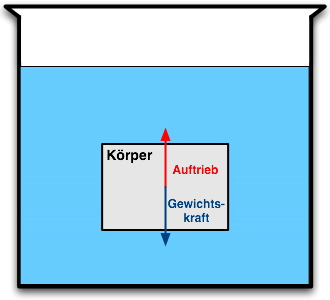
\includegraphics[width=0.75\linewidth]{Bilder/auftrieb} \\
\end{minipage}




	\begin{tabular}{c l c}
		$F_A$ & Auftriebskraft & $[F_A] = \mathrm{N}$ \\
		\rule{0pt}{8pt}$\rho_{Fl}$ & Dichte \textbf{verdrängtes Fluid} & $[\rho_{Fl}] = \mathrm{\frac{kg}{m^3}}$ \\
		$V_K$ & verdrängtes Fluid-Volumen & $[V_K] = \mathrm{m^3}$  \\
		\rule{0pt}{8pt}$g$ & Erdbeschleunigung $g = 9.81 \mathrm{\frac{m}{s^2}}$ & $[g] = \mathrm{\frac{m}{s^2}}$ \\
		$m_{Fl}$ & Masse des \textbf{verdrängten Fluids} & $[m_{Fl}] = \mathrm{kg}$ \\
		$F_{G,Fl}$ & Gewichtskraft \textbf{verdrängtes Fluid} & $[F_{G,Fl}] = \mathrm{N}$ \\
	\end{tabular}
	


\subsection{Oberflächenspannung $\sigma$}

$$ \boxed{ \sigma := \frac{F}{l} } $$ 


	\begin{tabular}{c l c}
		\rule{0pt}{10pt}$\sigma$ & Oberflächenspannung & $[\sigma] = \mathrm{\frac{N}{m}} = \mathrm{\frac{J}{m^2}}$ \\
		$F$ & Kraft & $[F] = \mathrm{N} $ \\
		$l$ & Länge & $[l] = \mathrm{m}$  \\
		\\
	\end{tabular}
	
	\textbf{Die Länge $l$ entspricht der gesamten Berührungslänge  \\
	zwischen Flüssigkeit und Festkörper / Gas} \\
	
	\begin{tabular}{ll}
	Zylinder & $l = 2 \, \pi \, r$ \\
	Lamellen & $l = 2 \, b$  (beidseitig!) \\
	\end{tabular}


\subsection{Grenzflächenspannung}

$$ \boxed{ \sigma_{sl} + \sigma_{lg} \cdot cos \varphi = \sigma_{sg }} $$

\begin{minipage}{0.48\linewidth}
	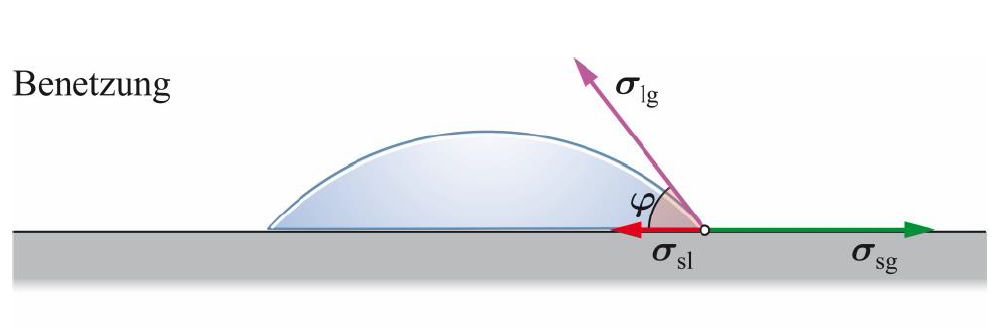
\includegraphics[width=\linewidth]{Bilder/benetzung.png} \\
	$ \varphi < 90 ^{\circ} $
\end{minipage}
\hfill
\begin{minipage}{0.48\linewidth}
	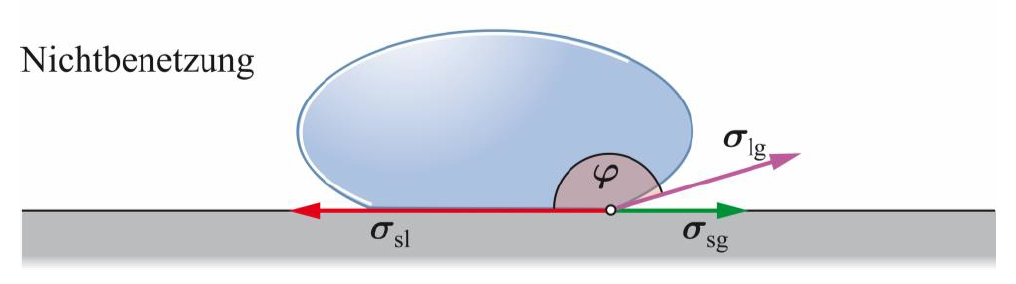
\includegraphics[width=\linewidth]{Bilder/nichtbenetzung.png} \\
	$ \varphi > 90° ^{\circ}$
\end{minipage}





\subsection{Kapillarität $h$}

$$\boxed{  h = \frac{2 \cdot \sigma}{\rho \cdot g \cdot r} = \frac{\sigma}{\rho \cdot g \cdot d} }$$ 


	\begin{tabular}{c l c}
		\rule{0pt}{10pt}$\sigma$ & Totale Grenzflächenspannung & $[\sigma] = \mathrm{\frac{N}{m}}$ \\
		\rule{0pt}{10pt}$\rho$ & Dichte der Flüssigkeit & $[\rho] = \mathrm{\frac{kg}{m^3}} $ \\
		\rule{0pt}{10pt}$r$ & Radius der Kapillare & $[r] = \mathrm{m}$  \\
		$d$ & Durchmesser der Kapillare & $[r] = \mathrm{m}$  \\
		\\
	\end{tabular}

\begin{minipage}{0.48\linewidth}
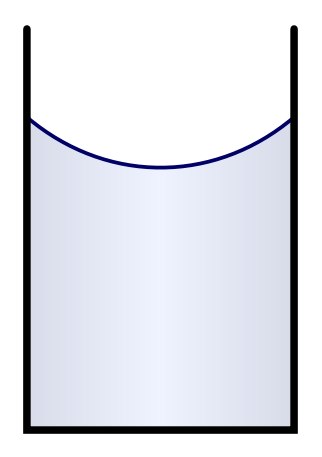
\includegraphics[width=0.3\linewidth]{Bilder/kapillaritaet_benetzend} \\

benetzend
\end{minipage}
\hfill
\begin{minipage}{0.48\linewidth}
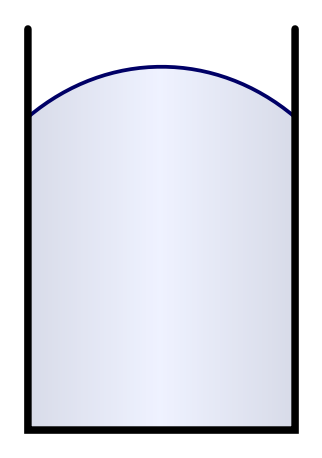
\includegraphics[width=0.3\linewidth]{Bilder/kapillaritaet_nicht_benetzend} \\

nicht benetzend

\end{minipage}




\subsection{Druck in Seifenblase $p$}

$$ \boxed{ p = \frac{2 \cdot \sigma}{r} } $$ 


	\begin{tabular}{c l c}
		\rule{0pt}{8pt}$\sigma$ & Oberflächenspannung & $[\sigma] = \mathrm{\frac{N}{m}}$ \\
		$r$ & Radius der Seifenblase & $[r] = \mathrm{m}$  \\
	\end{tabular}



% \vfill\null
% \columnbreak




\section{Hydrodynamik - Ideale Fluide}

\textbf{Ideale Fluide nehmen keine Scherkräfte auf (keine Reibung) und sind inkompressibel.}

\subsection{Stromlinien-Modell}

\begin{tabular}{ll}
$\bullet$ & Stromlinien zeigen Geschwindigkeit des Fluids \\
$\bullet$ & \textbf{Dichte} Stromlinien bedeutet \textbf{hohe} Geschwindigkeit \\
$\bullet$ & \textbf{Dünne} Stromlinien bedeutet \textbf{niedrige} Geschwindigkeit \\
$\bullet$ & Stationär: Stromlinien = Bahnlinien $\Rightarrow$ schneiden sich nicht 
\end{tabular}




\subsection{Kontinuitätsgleichung}


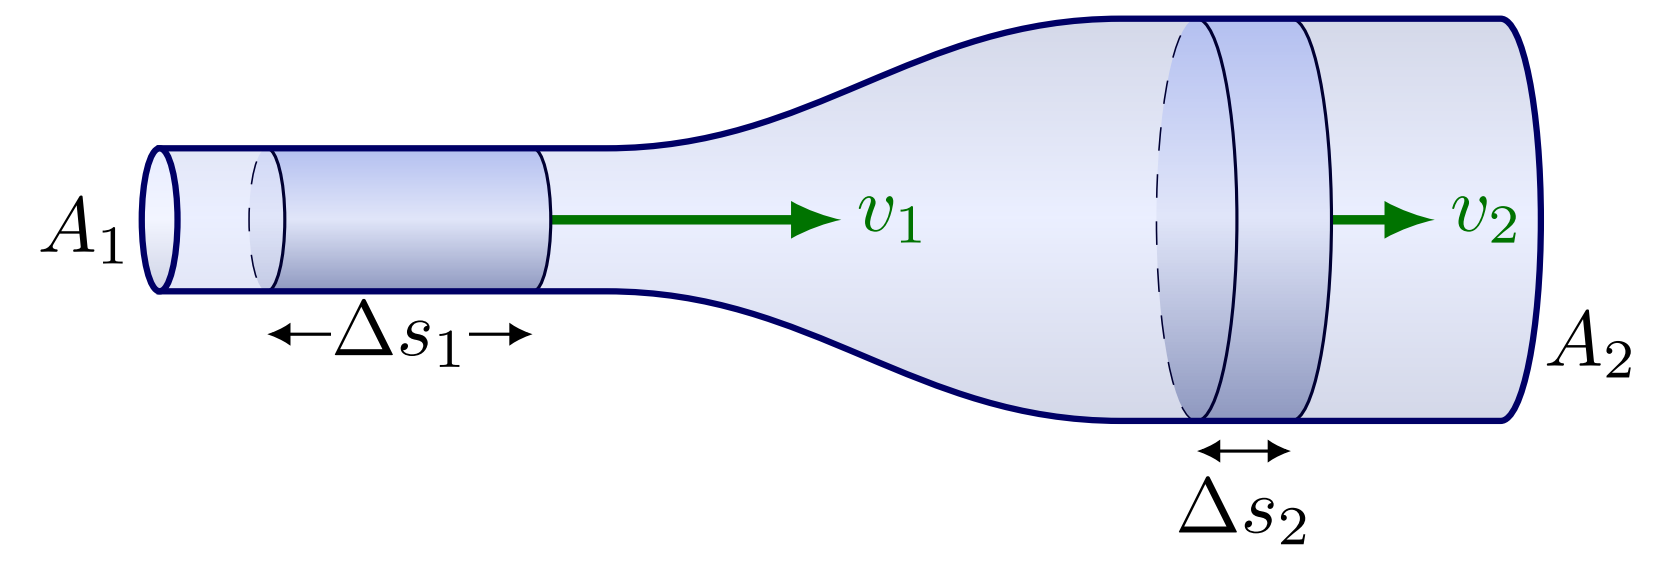
\includegraphics[width=0.7\linewidth]{Bilder/Kontinuitaet.png}


$$ \boxed{ \frac{\Delta V}{\Delta t} = \dot{V} = A \cdot v = \const } \quad \Leftrightarrow \quad \boxed{  A_1 \cdot v_1 = A_2 \cdot v_2 = \frac{\Delta V}{\Delta t} = \dot{V}} $$ 

\begin{tabular}{c l c}
		$\Delta V$ & Volumenänderung & $[\Delta V] = \mathrm{m^3}$ \\
		$\Delta t$ & Zeitänderung & $[\Delta t] = \mathrm{s}$  \\
		\rule{0pt}{8pt}$\dot{V}$ & Volumenstrom (Volumen pro Zeit) & $[\dot{V}] = \mathrm{\frac{m^3}{s}}$ \\
		$A_x$ & Querschnittsfläche & $[A_x] = \mathrm{m^2}$ \\
		\rule{0pt}{8pt}$v_x$ & Geschwindigkeit der Flüssigkeit & $[v_x] = \mathrm{\frac{m}{s}}$ \\
		\\
	\end{tabular}

$\Rightarrow$ Gilt auch für Gase, wenn $v << v_{Schall}$

% \vfill\null
% \columnbreak


\subsection{Bernoulli-Gleichung}

\begin{minipage}{0.38\linewidth}
Die Bernoulli-Gleichung beschreibt ein \\
\underline{bewegtes} Fluid \\
\end{minipage}
\hfill
\begin{minipage}{0.6\linewidth}
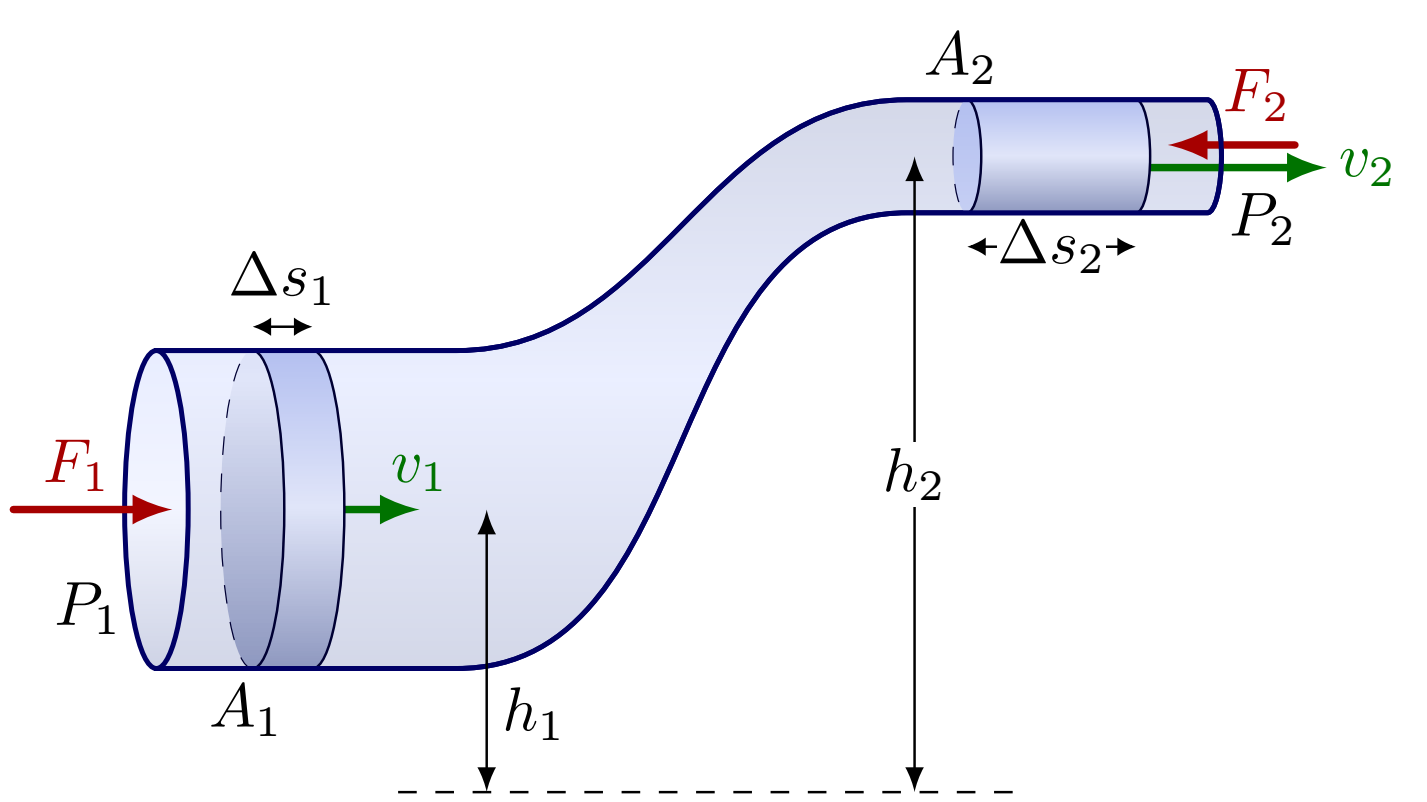
\includegraphics[width=0.99\linewidth]{Bilder/Bernoulli} \\
\end{minipage}








$$ \underbrace{ p + \rho \cdot g \cdot h }_{\substack{\mathrm{statisch}}} + \underbrace{ \frac{1}{2} \, \rho \cdot v^2 }_{\substack{\mathrm{dynamisch}}} = \const $$
	
	$$ \boxed{ p_1 +  \rho \cdot g \cdot h_1 + \frac{1}{2} \, \rho \cdot v_1^2 = p_2 +  \rho \cdot g \cdot h_2 + \frac{1}{2} \, \rho \cdot v_2^2 } $$


\subsubsection{Spezialfall: Horizontal}

$$ \boxed{ p + \frac{1}{2} \, \rho \cdot v^2 = \const } $$


\subsubsection{Spezialfall: Statik}

$$  \boxed{ p + \rho \, \cdot g \cdot h =  \const} $$




\subsubsection{Hydrodynamisches Paradoxon}
\textbf{Je grösser die Strömungsgeschwindigkeit, desto kleiner der Druck} \\


%\vfill\null
%\columnbreak



\subsection{Bernoulli-Gleichung und Energieerhaltung} % eventuell weglassen
Die in der Bernoulli-Gleichung vorkommenden Terme können als \underline{Energie pro Volumen} betrachtet werden \\
\\
\begin{tabular}{l c l}
$  \mathrm{E_{Mech}}$ & $=$ & $\mathrm{elast. \; Energie +  pot. \; Energie + kin. \; Energie}$ \\
\\
& $=$ & $ p \cdot V + m \cdot g \cdot h + \frac{1}{2} \, m \cdot v^2 = \const$ \\
\\
\end{tabular}


Wenn durch das Volumen dividiert wird erhält man: \\
\\
\begin{tabular}{l c l}
$  \mathrm{\frac{E_{Mech}}{Volumen}}$ & $=$ & $\mathrm{\frac{elatische Energie}{Volumen}   + \frac{pot. \; Energie}{Volumen} + \frac{kin. \; Energie}{Volumen}}$ \\
\\
& $=$ & $ p + \rho \cdot g \cdot h + \frac{1}{2} \,  \rho \cdot v^2 =\const$ \\
\\
\end{tabular}


Bei einer horizontalen Strömung entfällt die pot. Energie\\
(pro Volumen) \\
\\

\begin{tabular}{l c l}
$ \mathrm{ \frac{E_{Mech}}{Volumen}}$ & $=$ & $\mathrm{ \frac{elatische Energie}{Volumen} + \frac{kin. \; Energie}{Volumen} }$ \\
\\
& $=$ & $ p + \frac{1}{2} \, \rho \cdot v^2 = \const$ \\
\end{tabular}





\section{Hydrodynamik - Reale Fluide}

\textbf{Reale Fluide nehmen Scherkräfte auf (Reibung)}


\subsection{Newton'sches Reibungs-Gesetz}
Ein \underline{reales Fluid} erfährt \underline{Reibung} 

$$ \boxed{ \tau = \eta \cdot \frac{v}{d} }  \qquad  \boxed{ \tau = \eta \cdot \frac{d \, v}{d \, z} } $$

\begin{tabular}{c l c}
		$\tau$ & Schubspannung & $[\tau] = \mathrm{N}$ \\
		$\eta$ & dynmaische Zähigkeit (Viskosität) & $[\eta] = \mathrm{Pa \cdot s}$ \\
		\rule{0pt}{8pt}$v$ & Geschwindigkeitsdifferenz zw. Auflagen & $[v] = \frac{m}{s}$ \\
		$z$ & Richtung senkrecht zur Verschiebung & $[z] = \mathrm{m}$ \\
		$d$ & Distand zwischen den Auflagen & $[d] = \mathrm{m}$ \\
		\rule{0pt}{8pt}$\frac{d \, v}{d \, z}$ & Geschwindigkeits-Gradient in z-Richtung & $[\frac{d \, v}{d \, z}] = \mathrm{\frac{1}{s}}$ \\
		\\
\end{tabular}
	
\textbf{Beispiele: Werte für $\eta$} \\
\\
\begin{tabular}{l c l}
		$\eta_{Luft}$ & $:=$ & $17 \cdot 10^{-6} \; \mathrm{Pa \cdot s} $ \\
		$\eta_{Wasser} (20^{\circ}C)$ & $:=$ & $10^{-2} \; \mathrm{Pa \cdot s}$ \\
		$\eta_{Oel}$ & $:=$ & $0.1 \; \mathrm{Pa \cdot s}$ bis $1 \; \mathrm{Pa \cdot s}$ \\
\end{tabular}


\subsubsection{Kinematische Zähigkeit $\nu$}

$$ \boxed{ \nu = \frac{\eta}{\rho}  } $$

\begin{tabular}{c l c}
		\rule{0pt}{8pt}$\nu$ & kinematische Zähigkeit & $[\nu] = \mathrm{\frac{m^2}{s}}$ \\
		\rule{0pt}{8pt}$\rho$ & Dichte & $[\rho] = \mathrm{\frac{kg}{m^3}}$  \\	
\end{tabular}
	

	
\subsection{Stokes'sche Reibung $F_R$}
Z.B. für Kugel in Öl oder fallende Wassertropfen

$$ \boxed{ F_R = 6 \cdot \pi \cdot \eta \cdot R \cdot v } $$

\begin{tabular}{c l c}
		$F_R$ & Reibungskraft & $[F_R] = \mathrm{N}$ \\
		$\eta$ & Dynamische Zähigkeit (Viskosität) & $[\eta] = \mathrm{Pa \cdot s}$  \\
		$R$ & Kugelradius & $[R] = \mathrm{m}$ \\
		\rule{0pt}{8pt}$v$ & Geschwindigkeit & $[v] = \mathrm{\frac{m}{s}}$		
\end{tabular}


\subsubsection{Kugelfall-Viskosimeter}
Auf eine Kugel, welche in einer Flüssigkeit hinabgleitet wirken \\
folgende Kräfte: \\
\\
\begin{minipage}{0.4\linewidth}
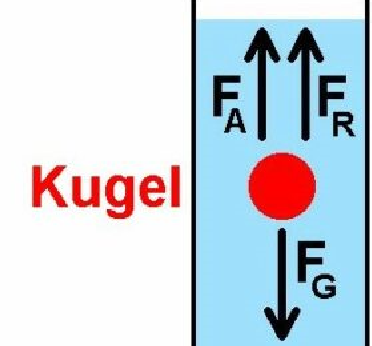
\includegraphics[width=0.8\linewidth]{Bilder/kugelfall-viskosimeter} \\
\end{minipage}
\hfill
\begin{minipage}{0.53\linewidth}
\begin{tabular}{ll}
$F_G$ & Gewichtskraft \\
$F_A$ & statischer Auftrieb \\
$F_R$ & Stokes'sche Reibung \\
\\
\end{tabular}

Ansatz zum Lösen von Aufgaben: \textbf{Kräftegleichgewicht}
\end{minipage}






% \vfill\null
% \columnbreak


\subsection{Hagen-Poiseuille}
Beschreibung von \underline{laminaren} Strömungen in einem \underline{runden Rohr} \\
$\Rightarrow$ Schichtströmung

\subsubsection{Gesetz von Hagen-Poiseuille}

$$ \boxed{ \dot{V} = \frac{\pi \cdot \Delta \, p \cdot R^4}{8 \cdot \eta \cdot l} } $$
 
\subsubsection{Geschwindigkeitsverteilung von $r=0$ bis R}

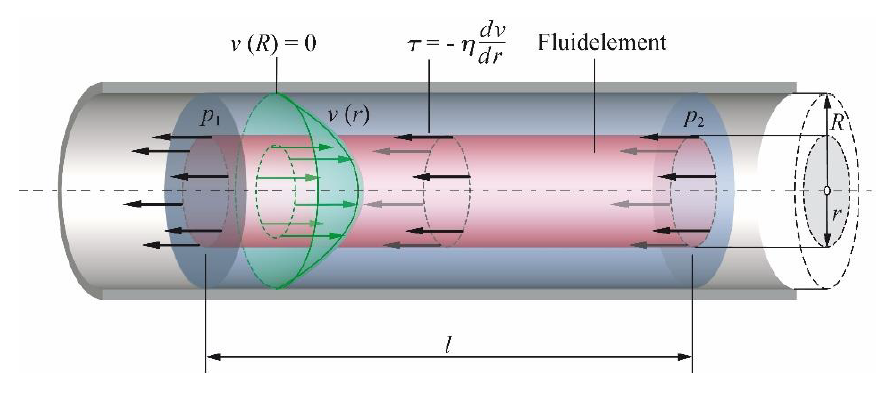
\includegraphics[width=0.8\linewidth]{Bilder/laminare_geschwindigkeit.png}

$$ \boxed{ v(r) = \frac{1}{4 \cdot \eta} \cdot \frac{\Delta \, p}{l} \, (R^2 - r^2) } $$



\begin{tabular}{c l c}
		\rule{0pt}{8pt}$v(r)$ & Fliessgeschwindigkeit beim Radius $r$ & $[v(r)] = \mathrm{\frac{m}{s}}$ \\
		$r$ & betrachteter Radius & $[r] = \mathrm{m}$ \\
		$\eta$ & Dynamische Zähigkeit (Viskosität) & $[\eta] = \mathrm{Pa \cdot s}$  \\
		$R$ & Rohr-(Innen)Radius & $[R] = \mathrm{m}$ \\
		$\Delta \, p$ & Druckdifferenz & $[\Delta \, p] = \mathrm{Pa}$ \\
		\rule{0pt}{8pt}$\dot{V} = \frac{d \, V}{d \, t}$ &  Volumenstrom & $[\dot{V}] = \mathrm{\frac{m^3}{s}}$	 \\
		$l$ & Länge des Rohrs & $[l] = \mathrm{m}$
\end{tabular}



\subsection{Reynolds-Zahl $Re$}
Gibt ein Richtmass für die Wirbelbildung  \\
\\
$\bullet$ Druck-Differenz (Bernoulli) begünstigt Wirbelbildung \\
$\bullet$ Innere Reibung (Schubspannung) verhindert Wirbelbildung 

$$\boxed{  Re = \frac{\Delta \, p}{\tau} = \frac{\rho \cdot \overline{v} \cdot d}{\eta} \qquad \qquad \mathrm{mit} \; \; \overline{v} = \frac{\dot{V}}{A} }  $$

	
\begin{tabular}{c l c}
		$Re$ & Reynolds-Zahl & $[Re] = 1$ \\
		$\eta$ & Dynamische Zähigkeit (Viskosität) & $[\eta] = \mathrm{Pa \cdot s}$  \\
		$\overline{v}$ & Mittlere Geschwindigkeit & $[\overline{v}] = \mathrm{\frac{m}{s}}$ \\
		$d$ & Typische Dimension (Rohrdurchmesser) & $[d] = \mathrm{m}$ \\
		$\Delta \, p$ & Druckdifferenz & $[\Delta p] = \mathrm{Pa}$ \\
		$\tau$ & Schubspannung & $[\tau] = \mathrm{N}$ \\
		\\
\end{tabular}

\textbf{Sobald die Reynolds-Zahl $Re$ grösser ist als ein kritischer Wert bilden sich Wirbel} \\
\\
$\Rightarrow$ Rohr:  $Re_{kritisch} \approx 2320$


\subsubsection{Ähnlichkeitsgesetz}
Reynolds-Zahl dient auch richtigem Vergleich von Modellversuchen. \\
\\
$\Rightarrow$ Gleiche Reynolds-Zahl bedeutet gleiches Verhalten \\
\\
$\Rightarrow$ Gleiche Reynolds-Zahl bedeutet auch gleiche \\
 Relative Grenzschicht-Dicke $D$ (siehe \ref{Grenzschichtdicke})



\vfill\null
\columnbreak


\subsection{Turbulente / Laminare Rohrströmung}

\subsubsection{Hilfe, um Reynoldszahl zu bestimmen (laminar)}

$$ \boxed{ \Delta p = 32 \cdot \eta \cdot l \cdot \frac{v}{d^2} }  $$


\subsubsection{Druckunterschied in laminare / turbulente Strömung}

$$ \lambda_{turbulent} = \frac{0.316}{\sqrt[4]{Re}}  \qquad \qquad \lambda_{laminar} = \frac{64}{Re}  $$

$$ \boxed{ \Rightarrow \Delta p_x = \lambda_x \frac{l}{d} \cdot \frac{\rho}{2} \cdot v^2 } $$



\begin{tabular}{c l c}
		$\Delta \, p_x$ & Druckdifferenz (laminar/turbulent) & $[\Delta p] = \mathrm{Pa}$ \\
		$\eta$ & Dynamische Zähigkeit (Viskosität) & $[\eta] = \mathrm{Pa \cdot s}$  \\
		$l$ & Rohr-Länge & $[l] = \mathrm{m}$ \\
		\rule{0pt}{8pt}$v$ & Fliess-Geschwindigkeit & $[v] = \mathrm{\frac{m}{s}}$ \\
		$d$ & Rohr-Durchmesser & $[d] = \mathrm{m}$ \\		
		\rule{0pt}{8pt}$\rho$ & Dichte des Fluids & $[\rho] = \mathrm{\frac{kg}{m^3}}$ \\
		$Re$ & Reynolds-Zahl & $[Re] = 1$ \\
\end{tabular}




\subsubsection{Unbekannt / Gemischt (Pratische Anwendung)}
Vorgehen, wenn man nicht weiss, ob sich Wirbel bilden oder nicht \\
\\
\begin{tabular}{ll}
1. & Laminar rechnen (um fehlenden Parameter $\rho, \; v, \; d, \; \mathrm{oder} \; \eta$ \\
   &  zu bestimmen) \\
2. & Aus Resultat Reynolds-Zahl berechnen \\
3. & Mit kritischer Reynolds-Zahl vergleichen \\
4. & Beim \textbf{Überschreiten} $\Rightarrow$ Turbulent rechnen! \\
\end{tabular}



\subsection{Prandl'sche Grenzschicht-Dicke $D$}\label{Grenzschichtdicke}
Prandl'sche Grenzschicht-Dicke $D$ beschreibt, in welcher \textbf{Distanz} die \textbf{Geschwindigkeit} eines laminar bewegten Teils (z.B. ein \\
Flugzeugflügel) \textbf{Null} ist. 

$$\boxed{ D = \sqrt{\frac{\eta}{\rho} \cdot \frac{l}{v}} }$$


\begin{tabular}{c l c}
		$D$ & Prandl'sche Grenzschicht-Dicke & $[D] = \mathrm{m}$ \\
		$\eta$ & Dynamische Zähigkeit (Viskosität) & $[\eta] = \mathrm{Pa \cdot s}$  \\
		\rule{0pt}{8pt}$\rho$ & Dichte des Fluids & $[\rho] = \mathrm{\frac{kg}{m^3}}$ \\
		$l$ & Länge des bewegten Teils (in Richtung von $v$) & $[l] = \mathrm{m}$ \\
		\rule{0pt}{8pt}$v$ & Geschwindigkeit & $[v] = \mathrm{\frac{m}{s}}$ \\
			\\
\end{tabular}

\begin{minipage}{0.48\linewidth}
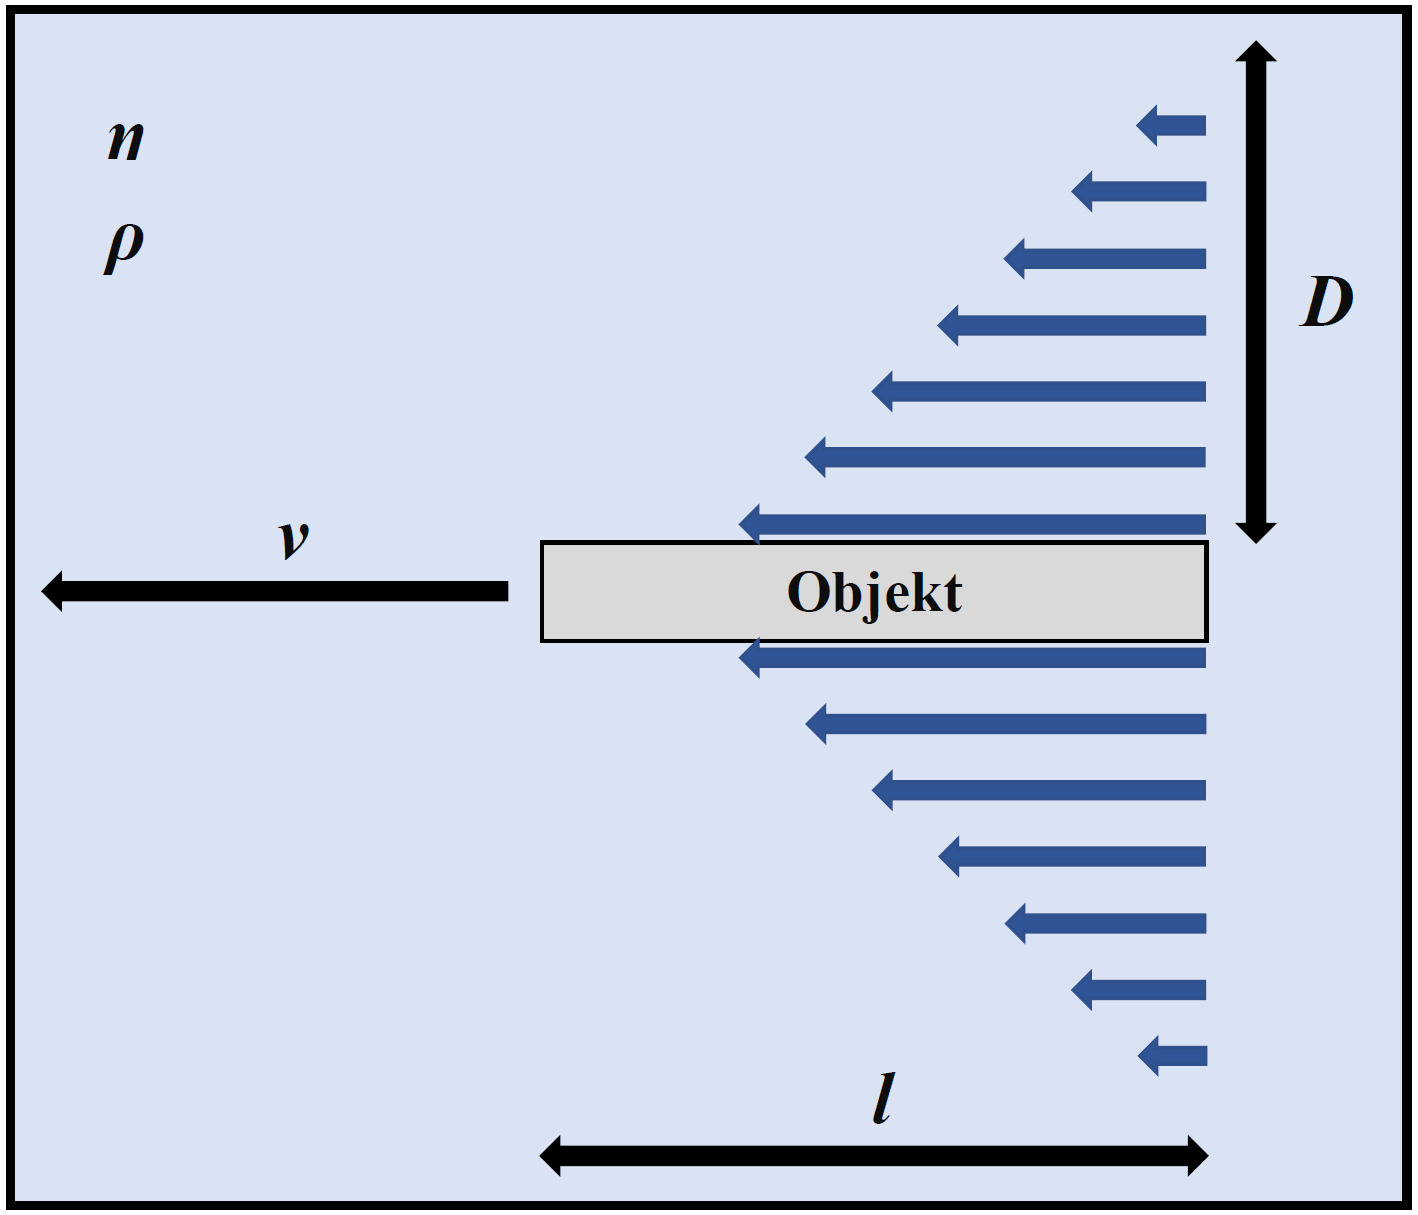
\includegraphics[width=0.8\linewidth]{Bilder/prandl}
\end{minipage}
\hfill
\begin{minipage}{0.48\linewidth}
Die Geschwindigkeit innerhalb der Grenzschicht $D$ nimmt vom Teil bis hin zum äussersten Rand \textbf{linear} ab.
\end{minipage}


% \vfill\null
% \columnbreak




\subsection{Bernoulli-Gleichung mit innerer Reibung}

$$ \boxed{  p_1 +  \rho \cdot g \cdot h_1 + \frac{1}{2} \, \textcolor{red}{\alpha_1} \cdot \rho \cdot v_1^2 = p_2 +  \rho \cdot g \cdot h_2 + \frac{1}{2} \, \textcolor{red}{\alpha_2} \cdot \rho \cdot v_2^2 \textcolor{red}{+ \Delta \, p_v}  }$$

\begin{tabular}{c| c |c}
 & turbulent & laminar \\ 
\hline 
Korrekturfaktoren & $\alpha_1 \approx \alpha_2 \approx 2$  & $\alpha_1 \approx \alpha_2 \approx 1$ \\ 
\hline 
\rule{0pt}{11pt} Druckverlust $\Delta \, p_v$ & \multicolumn{2}{c}{$\Delta p_v = \lambda_x \frac{l}{d} \cdot \frac{\rho}{2} \cdot v^2$} \\ 
\hline 
\rule{0pt}{11pt}  & $\lambda_{turbulent} = \frac{0.316}{\sqrt[4]{Re}}  $ & $\lambda_{laminar} = \frac{64}{Re} $  \\ 
\end{tabular} 



\subsection{Druckwiderstand $F_D$}
Bezeichnet die turbulente Luftreibungskraft $F_D$ und wird meist als Luftwiderstand bezeichnet \\

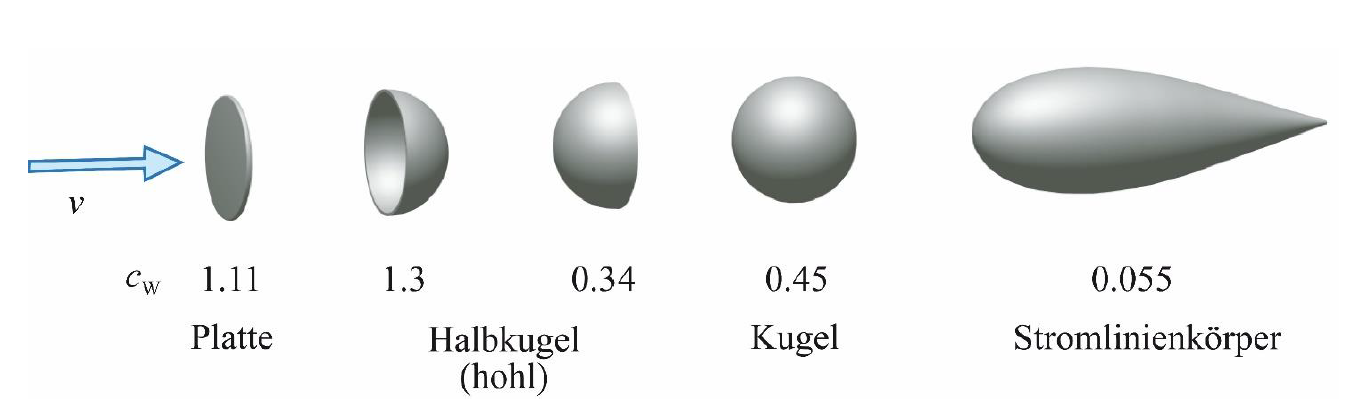
\includegraphics[width=0.8\linewidth]{Bilder/widerstandsbeiwert.png}

$$ \boxed{ F_D = \Delta \, p \cdot A_s = \frac{1}{2} \, \cdot \rho \cdot v^2 \cdot A_s \cdot c_W } $$


\begin{tabular}{c l c}
		$F_D$ & Druckwiderstand & $[F_D] = \mathrm{N}$ \\
		$\Delta \, p$ & Druckdifferenz & $[\Delta \, p] = \mathrm{Pa}$  \\
		\rule{0pt}{8pt}$\rho$ & Luft-Dichte & $[\rho] = \mathrm{\frac{kg}{m^3}}$ \\
		\rule{0pt}{8pt}$v$ & Strömungs-Geschwindigkeit & $[v] = \mathrm{\frac{m}{s}}$ \\
		$c_W$ & Widerstandsbeiwert / Widerstandszahl & $[c_W] = 1$\\
		$A_s$ & projizierte Fläche senkrecht zur Strömung & $[A_s] = \mathrm{m^2}$ \\
		\\
\end{tabular}

Der Widerstandsbeiwert $c_W$ ist \textbf{geometrieabhängig}!






\subsection{Auftriebskraft $F_A$ nach Kutta-Jukowski}
Beschreibt Proportionalität zwischen dynamischem Auftrieb \\
und Zirkulation 

$$ \boxed{ F_A = \rho \cdot v \cdot l \cdot \Gamma } $$

\begin{tabular}{c l c}
		$F_A$ & dynamischer Auftrieb & $[F_A] = \mathrm{N}$ \\
		\rule{0pt}{8pt}$\rho$ & Dichte des Fluids & $[\rho] = \mathrm{\frac{kg}{m^3}}$ \\
		\rule{0pt}{8pt}$v$ & Geschwindigkeit & $[v] = \mathrm{\frac{m}{s}}$ \\
		$l$ & Länge quer zur Strömung & $[l] = \mathrm{m}$ \\
		\rule{0pt}{8pt}$\Gamma$ & Zirkulation & $[\Gamma] = \mathrm{\frac{m^2}{s}}$ \\
\end{tabular}






\subsubsection{Zirkulation $\Gamma$}
Die Zirkulation ist ein Mass für die \textbf{Rotation} im Strömungsfeld \\

$$ \boxed{ \Gamma = 	\oint \vec{v} \bullet d\vec{s} } $$


\begin{tabular}{c l c}
		\rule{0pt}{8pt}$\Gamma$ & Zirkulation & $[\Gamma] = \mathrm{\frac{m^2}{s}}$ \\
		\rule{0pt}{8pt}$\vec{v} \bullet d\vec{s}$ & Geschwindigkeit entlang dem Weg & $[\vec{v}] = \mathrm{\frac{m}{s}}$  \\
		& (Skalarprodukt: $\vec{v} \bullet d\vec{s} = a \cdot b \cdot \cos(\varphi)$ & \\
\end{tabular} \\
\\
\textbf{Rotierender Zylinder:} $$ \boxed{ \Gamma = 2\pi r v_{Zyl} = 4\pi^2r^2f } $$


% \vfill\null
% \columnbreak



\subsection{Dynamischer Auftrieb $F_A$}

$$ \boxed{ F_A = c_A \cdot  \underbrace{\frac{1}{2} \cdot \rho \cdot v^2 }_{\substack{\Delta \, p}} \cdot A_{\|}	} $$


\begin{tabular}{c l c}
		$F_A$ & dynamischer Auftrieb & $[F_A] = \mathrm{N}$ \\
		$c_A$ & Auftriebskoeffizient & $[c_A] = 1$ \\
		\rule{0pt}{8pt}$\rho$ & Luft-Dichte & $[\rho] = \mathrm{\frac{kg}{m^3}}$ \\
		\rule{0pt}{8pt}$v$ & Strömungsgeschwindigkeit & $[v] = \mathrm{\frac{m}{s}}$ \\
		$A_{\|}$ & Projizierte Fläche \textbf{parallel} zur Strömung & $[A_{\|}] = \mathrm{m^2}$ \\
\end{tabular}




\subsubsection{Wissenswertes zum dynamischen Auftrieb}
Ein gerade ausgerichtetes, symmetrisches Stromlinienprofil erzeugt \textbf{keinen} dynamischen Auftrieb \\
\\
An einem asymmetrischen Flügelprofil entsteht dynamischer\\
Auftrieb 


\subsection{Induzierter Widerstand $F_W$}
Kommt durch Energieverlust (Wirbelbildung) zu Stande, welcher entsteht, wenn die Umgebungsluft in Bewegung gesetzt wird

$$ \boxed{ F_W = c^*_W \cdot \frac{1}{2} \cdot \rho \cdot v^2 \cdot A_{\|} } $$


\begin{tabular}{c l c}
		$F_W$ & Induzierter Widerstand & $[F_W] = \mathrm{N}$ \\
		$c^*_W$ & Widerstands-Koeffizient & $[c*_W] = 1$ \\
		\rule{0pt}{8pt}$\rho$ & Luft-Dichte & $[\rho] = \mathrm{\frac{kg}{m^3}}$ \\
		\rule{0pt}{8pt}$v$ & Strömungsgeschwindigkeit & $[v] = \mathrm{\frac{m}{s}}$ \\
		$A_{\|}$ & Projizierte Fläche \textbf{parallel} zur Strömung & $[A_{\|}] = \mathrm{m^2}$ \\
\end{tabular}


\subsection{Gleitwinkel $\varphi$}
Gibt die zurückgelegte Stecke pro verbrauchte Höhe an \\
Im Luft-Kanal ist dies der Anstell-Winkel \\

\begin{minipage}{0.5\linewidth}
	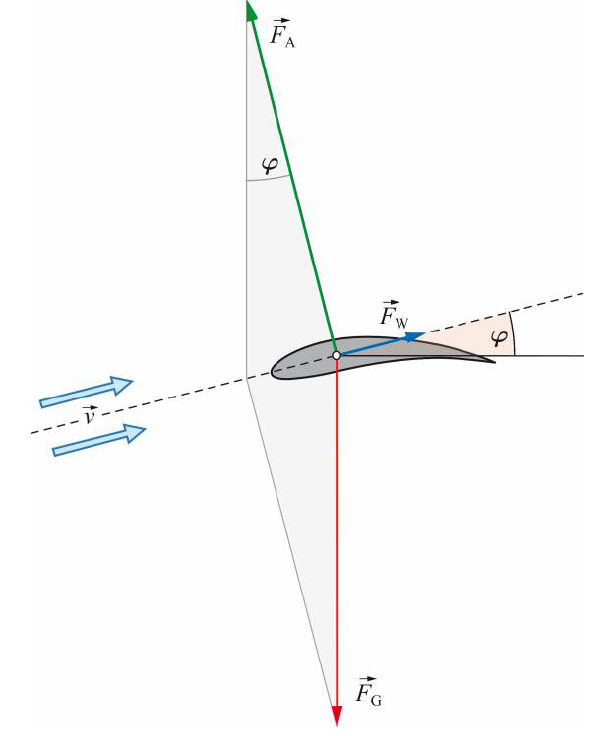
\includegraphics[width=\linewidth]{Bilder/gleitwinkel.png}
\end{minipage}
\hfill
\begin{minipage}{0.45\linewidth}
	$$ \boxed{ tan(\varphi) = \frac{F_W}{F_A} = \frac{c^*_W}{c_A}= \frac{v_V}{v_H} }	$$
\end{minipage}






\begin{tabular}{c l c}
		$\varphi$ & Gleitwinkel & $[\varphi] = \text{°}$ \\
		$F_W$ & Widerstandskraft & $[F_W] = \mathrm{N}$ \\
		$F_A$ & Auftriebskraft & $[F_A] = \mathrm{N}$ \\ 
		$c^*_W$ & Widerstands-Koeffizient & $[c^*_W] = 1$ \\
		$c_A$ & Auftriebs-Koeffizient & $[c_A] = 1$ \\
		\rule{0pt}{8pt}$v_V$ & Vertikal-Geschwindigkeit & $[v_V] = \mathrm{\frac{m}{s}}$ \\
		\rule{0pt}{8pt}$v_H$ & Horizontal-Geschwindigkeit & $[v_H] = \mathrm{\frac{m}{s}}$ \\
\end{tabular}

\subsubsection{Gängige Gleitzahlen}
\begin{center}
    \begin{tabular}{lc}
        \textbf{Flugobjekt} & \textbf{Gleitzahl}\\ \hline
		Hängegleiter  & 10 bis 15 \\
		Boeing 747    & 15 \\
		Airbus A380   & 20 \\
		Segelflugzeug &	40 (Rekord 70) \\
	\end{tabular}
\end{center}


\subsection{Helmholz'sche Wirbelsätze}
\begin{tabular}{ll}
1. & Wirbel hat kein Anfang und kein Ende \\
2. & Wirbel besteht immer aus denselben Fluidteilchen \\
3. & Zirkulation zeitlich konstant \\
\end{tabular}

% \vfill\null
% \columnbreak

		\section{Thermodynamik}

\subsection{Terminologie}

\begin{center}
    \begin{tabular}{l||l|lll}
        \textbf{System ist $\downarrow$} & \textbf{Materie-} & & \multicolumn{2}{l}{\textbf{Energietausch}}  \\
			& \textbf{tausch} &	& Arbeit & Wärme \\ \hline
		offen & erlaubt & - & erlaubt  & erlaubt \\
		      &         & adiabatisch  & erlaubt & Nein\\
			  &         & arbeitsdicht & Nein    & erlaubt\\
			  &         & beides       & Nein    & Nein\\ \hline
		geschlossen & Nein & - & möglich  & möglich \\
		      &         & adiabatisch  & möglich & Nein\\
			  &         & arbeitsdicht & Nein    & möglich\\
			  &         & energiedicht & Nein    & Nein\\
	\end{tabular}
\end{center}

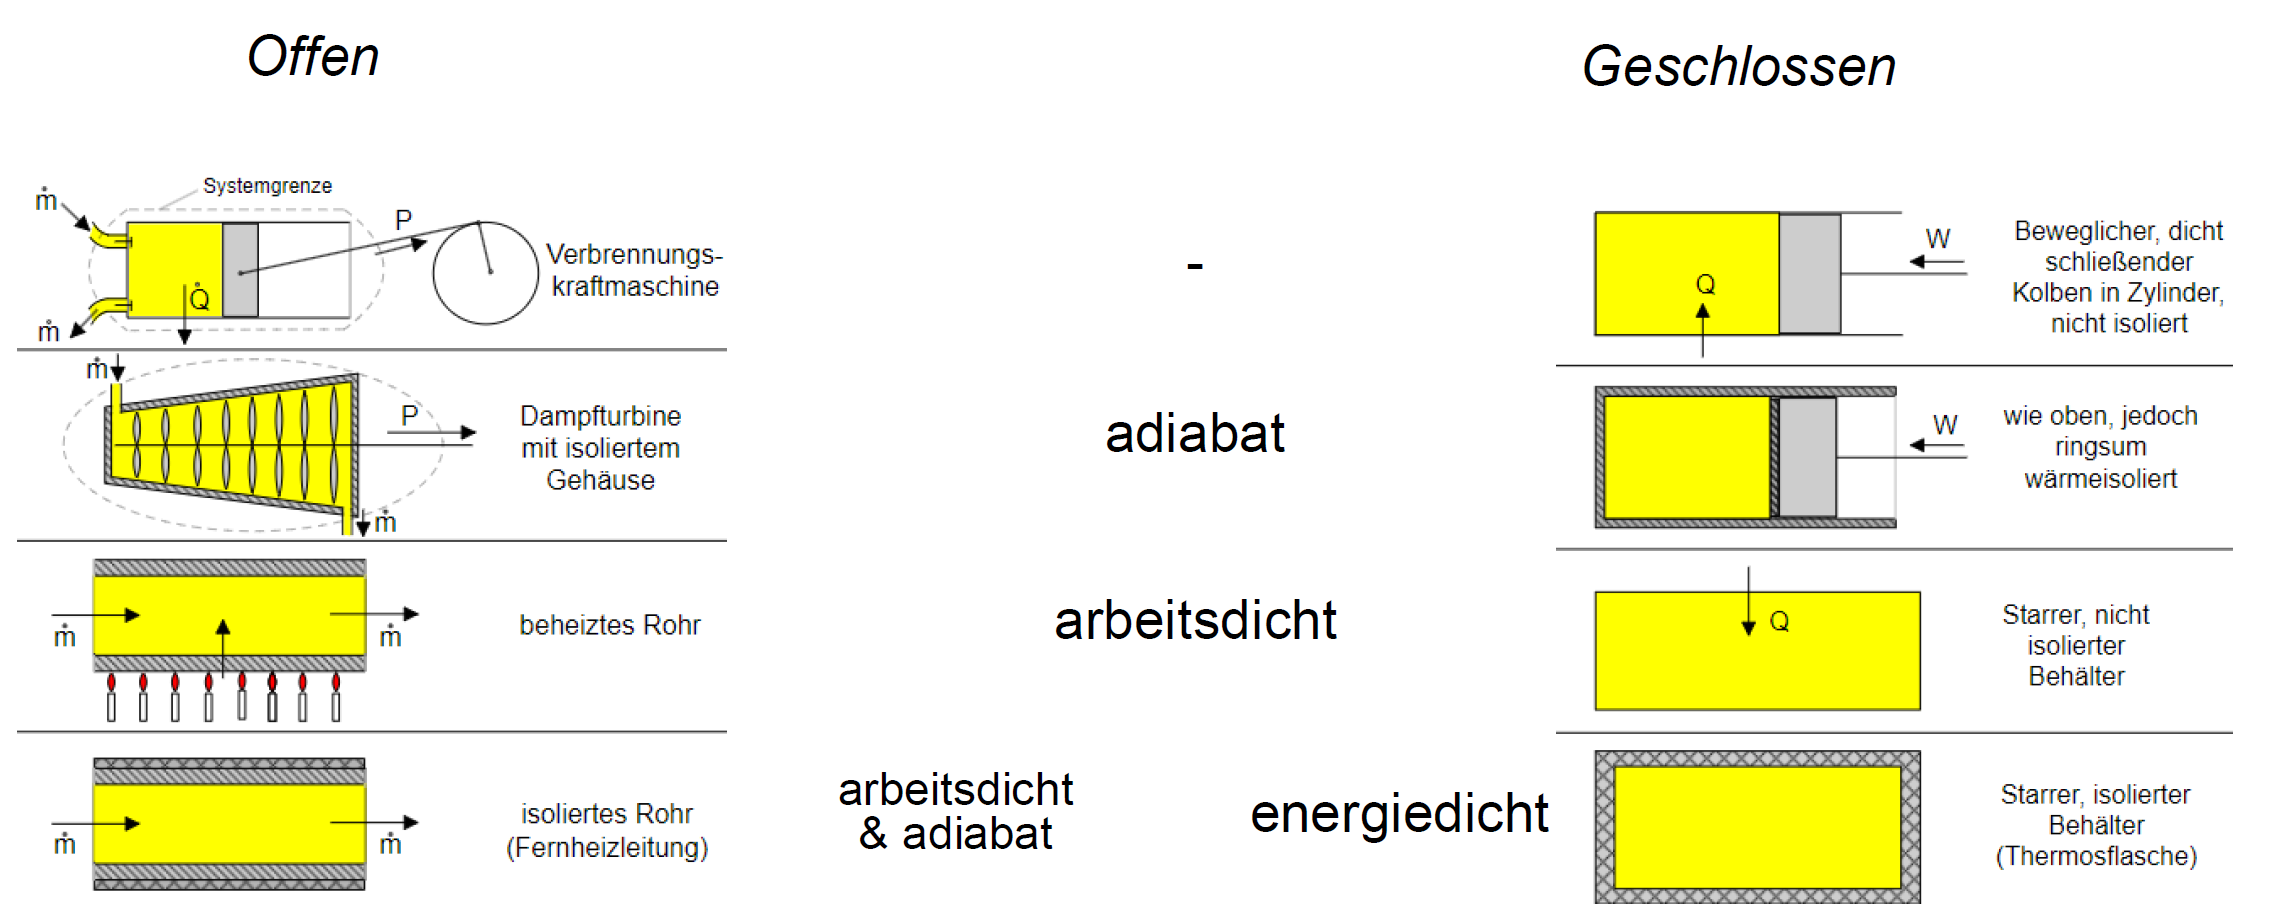
\includegraphics[width=\linewidth]{Bilder/thermodynamisches_system.png}

\subsection{Absolute Temperatur $T$}
$$ \boxed{ T = \theta + 273.15 \, K = \theta - \theta_0 }$$

\begin{tabular}{c l c}
		$T$ & Absolute Temperatur gemessen in Kelvin & $[T] =\mathrm{K}$  \\
		$\theta$ & Temperatur gemessen in °C & $[\theta] = \text{°C}$ \\
		$\theta_0$ & Absoluter Nullpunkt: $= -273.15 \,  \text{°C} = 0 \, \mathrm{K}$  &  \\
\end{tabular}




\subsection{Thermische Ausdehnung}

\subsubsection{Längenausdehnung $\Delta \, l $}

$$ \boxed{  l' = l + \Delta \,  l = l + \alpha \cdot l \cdot \Delta \, T = l\, (1 + \alpha \cdot \Delta \, T ) }$$


\begin{tabular}{c l c}
		$l'$ & Länge nach Ausdehnung & $[l'] = \mathrm{m}$ \\
		$l$ & Anfangslänge & $[l] = \mathrm{m}$ \\
		$\Delta \, l$ & Längenänderung & $[\Delta \, l] = \mathrm{m}$ \\
		\rule{0pt}{8pt}$\alpha$ & Längenausdehnungskoeffizient & $[\alpha] = \mathrm{\frac{1}{K}}$ \\ 
		$\Delta \, T $ & Temperaturänderung & $[\Delta \, T ] = \mathrm{K}$ \\
\end{tabular}


\subsubsection{Flächenausdehnung $\Delta \, A $}

$$ \boxed{ A' = A + \Delta \,  A = A + \underbrace{  \beta }_{\substack{\approx 2 \, \alpha}}  \cdot A \cdot \Delta \, T = A\, (1 + \beta \cdot \Delta \, T ) } $$


\begin{tabular}{c l c}
		$A'$ & Länge nach Ausdehnung & $[A'] = \mathrm{m^2}$ \\
		$A$ & Anfangslänge & $[A] = \mathrm{m^2}$ \\
		$\Delta \, A$ & Längenänderung & $[\Delta \, A] = \mathrm{m^2}$ \\
		\rule{0pt}{8pt}$\beta$ & Flächenausdehnungskoeffizient & $[\beta] = \mathrm{\frac{1}{K}}$ \\ 
		$\Delta \, T $ & Temperaturänderung & $[\Delta \, T ] = \mathrm{K}$ \\
\end{tabular}



\subsubsection{Volumenausdehnung $\Delta \, V $}

$$ \boxed{ V' = V + \Delta \,  V = V + \underbrace{  \gamma }_{\substack{\approx 3 \, \alpha}}  \cdot V \cdot \Delta \, T = V \, (1 + \gamma \cdot \Delta \, T ) }$$


\begin{tabular}{c l c}
		$V'$ & Volumen nach Ausdehnung & $[V'] = \mathrm{m^3}$ \\
		$V$ & Anfangsvolumen & $[V] = \mathrm{m^3}$ \\
		$\Delta \, V$ & Volumenänderung & $[\Delta \, V] = \mathrm{m^3}$ \\
		\rule{0pt}{8pt}$\gamma$ & Volumenausdehnungskoeffizient & $[\gamma] = \mathrm{\frac{1}{K}}$ \\ 
		$\Delta \, T $ & Temperaturänderung & $[\Delta \, T ] = \mathrm{K}$ \\
\end{tabular}

% \vfill\null
% \columnbreak

\begin{center}
    \begin{tabular}{lc}
        \textbf{Material} & \textbf{Koeffizient ($10^{-6} K^{-1} $)}\\ \hline
		Aluminium       & 23 \\
		Eisen           & 12 \\
		Stahl, unlegiert& 11 ... 13 \\
		Diamant         & 1.3 \\
		Silizium        & 2 \\
		Gummi           & 220 \\
		Beton           & 12 \\
		Polysterol      & 70 \\
		Zerodur         & 0 $\pm$ 0.007 \\
	\end{tabular}
\end{center}




\subsection{Thermische Spannung $\sigma$}


$$\boxed{  p = \sigma = \varepsilon \cdot E = E \cdot \frac{\Delta l}{l} =  E \cdot \alpha \cdot \Delta \, T } $$

\begin{tabular}{c l c}
		$\sigma$ & Thermische Spannung & $[\sigma] = \mathrm{Pa}$ \\
		$\varepsilon$ & Dehnung & $[\varepsilon] = 1$ \\
		\rule{0pt}{8pt}$E$ & Elastizitätsmodul & $[E] = \mathrm{\frac{N}{m^2}}$ \\
		\rule{0pt}{8pt}$\alpha$ & Längenausdehnungskoeffizient & $[\alpha] = \mathrm{\frac{1}{K}}$ \\ 
		$\Delta \, T $ & Temperaturänderung & $[\Delta \, T ] = \mathrm{K}$ \\
		$p$ & Druck & $[p] = \mathrm{Pa} $ \\
\end{tabular}






\section{Ideales Gas}

\subsection{Modell des idealen Gases}
\textbf{Jedes Gas ist gleich!} \\


\begin{tabular}{ll}
$1.$ & Moleküle sind Massepunkte (keine Ausdehnung) \\
$2.$ & Stösse sind elastisch (keine zwischenmolekularen Kräfte) \\
& Kein Volumen bei $T = 0$ \\
& Kein Druck bei $T = 0$ \\
\end{tabular}





\subsubsection{Thermische Ausdehnung von Gasen}
\begin{tabular}{ll}
$\bullet$ & Ausdehnung von Gasen ist sehr gross \\
$\bullet$ & Bei \textbf{allen} Gasen ist die Ausdehnung \textbf{gleich} \\
$\bullet$ & Volumen beim Nullpunkt ist \textbf{Null} \\
\end{tabular}


\vfill\null
\columnbreak

\subsection{Universelle Gasgleichung}
Alle Gase verhalten sich gleich, insbesondere bei gleicher Anzahl Moleküle \\


$$ \boxed{ \frac{p \cdot V}{T} = \, \const } \qquad  \Rightarrow \boxed{ \frac{p_1 \cdot V_1}{T_1} = \frac{p_2 \cdot V_2}{T_2} } $$ 


\begin{tabular}{c l c}
	$p_x$ & \textbf{Absolut-}Druck & $[p_x] = \mathrm{Pa}$ \\
	& Absolut-Druck: $p_0 + p$ \\
	$V_x$ & Volumen & $[V_x] = \mathrm{m^3}$ \\
	$T_x$ & \textbf{Absolut-}Temperatur (in K) & $[T] = \mathrm{K}$ \\
\end{tabular}
	
% \vfill\null
% \columnbreak

	
\subsubsection{Boyle-Mariotte}	
\textbf{Das Gesetz gilt nur bei konstanter Temperatur!} \\
$\Rightarrow$ \textbf{Isotherme} Zustandsänderung

$$  \boxed{ p \cdot V = \, \const } \qquad  \Rightarrow  \boxed{ p_1 \cdot V_1 = p_2 \cdot V_2 } $$ 





\subsubsection{Gay-Lussac}

\textbf{ Das Gesetz gilt nur bei konstantem Druck!} \\
$\Rightarrow$ \textbf{Isobare} Zustandsänderung

$$  \boxed{ \frac{V}{T} = \; \const } \qquad  \Rightarrow  \boxed{ \frac{V_1}{T_1} = \frac{V_2}{T_2} } $$


	
	
\subsubsection{Gay-Lussac und Amontons}

\textbf{Das Gesetz gilt nur bei konstantem Volumen!} \\
$\Rightarrow$ \textbf{Isochore} Zustandsänderung

$$ \boxed{ \frac{p}{T} = \; \const } \qquad  \Rightarrow \boxed{ \frac{p_1}{T_1} = \frac{p_2}{T_2} }$$


	
\subsection{Universelle Gasgleichung für ideale Gase}\label{Gasgleichung ideal}

$$ \boxed{ p \cdot V = n \cdot R \cdot T = N \cdot k \cdot T }$$
	
	
\begin{tabular}{c l c}
	$p$ & \textbf{Absolut-}Druck & $[p] = \mathrm{Pa}$ \\
	    & Absolut-Druck: $p_0 + p$ & \\
	$V$ & Volumen & $[V] = \mathrm{m^3}$ \\
	$n$ & Mol-Zahl & $[n] = \mathrm{mol}$ \\
	\rule{0pt}{8pt}$R$ & Universelle Gaskonstante: $R = 8.314 \mathrm{\frac{J}{mol \cdot K}}$ & $[R] = \mathrm{\frac{J}{mol \cdot K}} $ \\
	$T$ & \textbf{Absolut-}Temperatur (in K) & $[T] = \mathrm{K}$ \\
	$N$ & Anzahl Moleküle & $[N] = 1$ \\
	\rule{0pt}{8pt}$k$ & Boltzmann-Konstante $k = 1.381 \cdot 10^{-23} \mathrm{\frac{J}{K}}$ & $[k] = \mathrm{\frac{J}{K}}$ \\
\end{tabular}
	
	
	
	
\subsubsection{Zusammenhänge zwischen den Konstanten}
	
$$  \boxed{ R = k \cdot N_A = \frac{N \cdot k}{n} } $$

$$\boxed{ n = \frac{N}{N_A} = \frac{m}{M} = \frac{N \cdot k}{R} } $$
	


\begin{tabular}{c l c}
	\rule{0pt}{8pt}$R$ & Universelle Gaskonstante: $R = 8.314 \mathrm{\frac{J}{mol \cdot K}}$ & $[R] = \mathrm{\frac{J}{mol \cdot K}} $ \\
	\rule{0pt}{8pt}$k$ & Boltzmann-Konstante $k = 1.381 \cdot 10^{-23} \mathrm{\frac{J}{K}}$ & $[k] = \mathrm{\frac{J}{K}}$ \\
	$N$ & Anzahl Moleküle & $[N] = 1$ \\
	\rule{0pt}{8pt}$N_A$ & 	Avogadrokonstante: $N_A = 6.022 \cdot 10^{23} \, \mathrm{\frac{1}{mol}} $ & $[N_A] =  \mathrm{\frac{1}{mol}}$  \\	
	$n$ & Mol-Zahl & $[n] = \mathrm{mol}$ \\
	$m$ & Masse & $[m] = \mathrm{kg}$ \\
	\rule{0pt}{8pt}$M$ & Mol-Masse & $[M] = \mathrm{\frac{kg}{mol}}$ \\
\end{tabular}

% \vfill\null
% \columnbreak


\subsection{Mechanische Arbeit $\Delta W$ von Gasen}
\label{MechArbeit}

Folgende Formel ist für Flüssigkeiten \textbf{nicht} gültig, da diese \\
inkompressibel sind ($\Delta V = 0$)


$$ \boxed{ \Delta W = F \cdot \Delta s = p \cdot A \cdot \Delta s = p \cdot \Delta V } $$
\\

\begin{tabular}{c l c}
	$\Delta W$ & Mechanische Arbeit von Gas & $[\Delta W] = \mathrm{J}$ \\
	$F$ & Kraft & $[F] = \mathrm{N}$ \\
	$\Delta s$ & Wegänderung & $[\Delta s] = \mathrm{m}$ \\
	$p$ & Druck & $[p] = \mathrm{Pa}$ \\
	$A$ & Fläche & $[A] = \mathrm{m^2}$ \\
	$\Delta V$ & Volumenänderung & $[\Delta V] = \mathrm{m^3}$ \\
\end{tabular}



\subsection{Gesetz von Avogadro}
Ein Mol eines Gases nimmt bei Normalbedingungen immer das \\
gleiche Volumen ein (=Molvolumen) \\
\\
Ideale Gase enthalten bei gleichem Druck p und gleicher \\
Temperatur T immer gleich viele Moleküle (im Molvolumen)





\subsection{Molmasse $M$, Molvolumen $V_m$}

Siehe auch \ref{Gasgleichung ideal}\\

Molmasse ist die \textbf{Ordnungszahl} im Periodensystem

$$  \boxed{ n = \frac{m}{M} = \frac{N}{N_A} } $$


Mol-Volumen:

$$ \boxed{ V_m = \frac{V}{n} }$$



\begin{tabular}{c l c}
	$p$ & \textbf{Absolut-}Druck & $[p] = \mathrm{Pa}$ \\
	    & Absolut-Druck: $p_0 + p$ & \\
	$V$ & Volumen & $[V] = \mathrm{m^3}$ \\
	\rule{0pt}{8pt}$R$ & Universelle Gaskonstante: $R = 8.314 \mathrm{\frac{J}{mol \cdot K}}$ & $[R] = \mathrm{\frac{J}{mol \cdot K}} $ \\
	$T$ & \textbf{Absolut-}Temperatur (in K) & $[T] = \mathrm{K}$ \\
	\rule{0pt}{8pt}$N_A$ & 	Avogadrokonstante: $N_A = 6.022 \cdot 10^{23} \, \mathrm{\frac{1}{mol}} $ & $[N_A] =  \mathrm{\frac{1}{mol}}$  \\	
	\rule{0pt}{8pt}$k$ & Boltzmann-Konstante $k = 1.381 \cdot 10^{-23} \mathrm{\frac{J}{K}}$ & $[k] = \mathrm{\frac{J}{K}}$ \\	
	$n$ & Mol-Zahl & $[n] = \mathrm{mol}$ \\
	$m$ & Masse & $[m] = \mathrm{kg}$ \\
	\rule{0pt}{8pt}$M$ & Mol-Masse & $[M] = \mathrm{\frac{kg}{mol}}$ \\
	$N$ & Anzahl Moleküle & $[N] = 1$ \\
	\rule{0pt}{8pt}$V_m$ & Mol-Volumen & $[V_m] = \mathrm{\frac{m^3}{mol}}$ \\
\end{tabular}

% \vfill\null
% \columnbreak



\subsection{Dichte eines Gases $\rho$}

$$ \boxed{ \rho = \frac{m}{V} = \frac{M}{V_m} = \frac{p \cdot M}{R \cdot T} }$$


\begin{tabular}{c l c}
	\rule{0pt}{8pt}$\rho$ & Gas-Dichte & $[\rho] = \mathrm{\frac{kg}{m^3}}$ \\
	$m$ & Masse & $[m] = \mathrm{kg}$ \\
	$V$ & Volumen & $[V] = \mathrm{m^3}$ \\
	\rule{0pt}{8pt}$M$ & Mol-Masse & $[M] = \mathrm{\frac{kg}{mol}}$ \\
	\rule{0pt}{8pt}$V_m$ & Mol-Volumen (22.4 L bei 0 °C und 1000 hPa) & $[V_m] = \mathrm{\frac{m^3}{mol}}$ \\
	\rule{0pt}{8pt}$p$ & \textbf{Absolut-}Druck & $[p] = \mathrm{Pa}$ \\
	    & Absolut-Druck: $p_0 + p$ & \\
	\rule{0pt}{8pt}$R$ & Universelle Gaskonstante: $R = 8.314 \mathrm{\frac{J}{mol \cdot K}}$ & $[R] = \mathrm{\frac{J}{mol \cdot K}} $ \\
	$T$ & \textbf{Absolut-}Temperatur (in K) & $[T] = \mathrm{K}$ \\
\end{tabular}



\subsection{Phänomene von idealen Gasen}

\subsubsection{Annomalie des Wassers}
Die feste Form (Eis) ist leichter als die flüssige Form (Wasser) \\
Die \textbf{grösste Dichte weist Wasser bei 4 °C} auf, nicht beim \\
 Gefrierpunkt von 0 °C \\

$\Rightarrow$ Ein See gefriert somit nur an der Oberfläche. Am Grund des Sees beträgt die Wassertemperatur 4 °C 


\subsubsection{Osmotischer Druck (Zelldruck)}

Grosse Moleküle innerhalb von vielen kleinen Molekülen in einer Flüssigkeit verhalten sich ähnlich wie die Moleküle eines idealen \\ Gases, wenn die Flüssigkeit von einer für die Müleküle \\
halb-durchlässigen (semi-permeabel) Membran umgeben ist.\\
\\
$ \mathrm{Osmotischer \; Druck:} \; p = \frac{n}{V} \cdot R \cdot T  \qquad \mathrm{(ideale \; Gasgleichung)}$

\vfill\null
\columnbreak

\subsection{Partialdruck $p_i$}
\textbf{Ausgangslage: Gasgemisch (z.B. Luft: Sauerstoff-Stickstoff)} \\
\\

\begin{minipage}{0.48\linewidth}
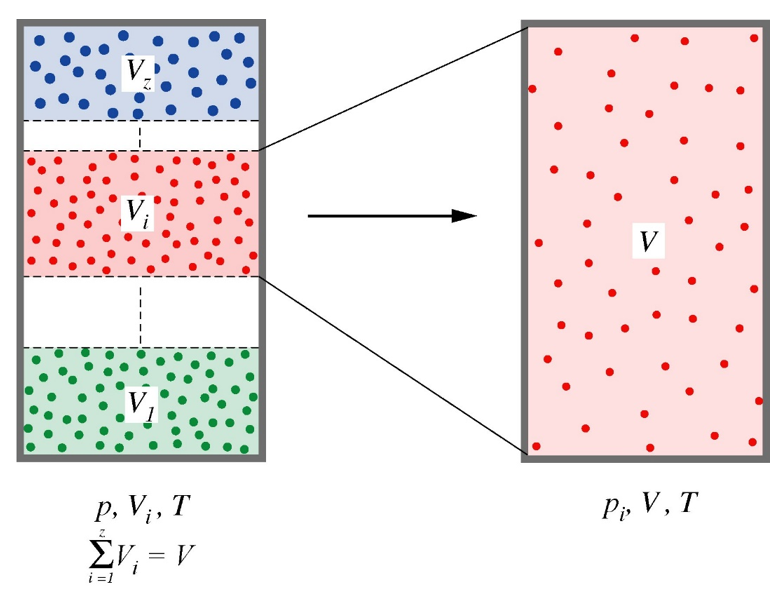
\includegraphics[width=\linewidth]{Bilder/partialdruck}
\end{minipage}
\hfill
\begin{minipage}{0.5\linewidth}
Der Partialdruck $p_i$ ist der Druck, welcher die i-te Gaskomponete erzeugen würde, wenn ihr das gesamte Volumen zur Verfügung stehen würde. \\
\end{minipage}

% \vfill\null
% \columnbreak

\subsection{Gesetz von Dalton}
In einem Gas ist die Summe der Partialdrücke $p_i$ gleich dem \\
Gesamtdruck 

$$ \boxed{ \sum_{i=1}^n  p_i = p } $$ 



\begin{tabular}{c l c}
	$p_i$ & Partialdruck & $[p_i] = \mathrm{Pa}$ \\
	$p$ & (Gesamt-) Druck & $[p] = \mathrm{Pa}$ \\
\end{tabular}


\subsection{Volumen- und Massenkonzentration (Gasgemisch)}


\subsubsection{Volumen-Konzentrationen (Volumen-Anteile)}


$$ \boxed{  q_i = \frac{V_i}{V} = \frac{n_i}{n} = \frac{p_i}{p} } $$


\begin{tabular}{c l c}
	$q_i$ & Volumen-Konzentration& $[q_i] = 1$ \\
	$V_i$ & Volumen der i-ten Gas-Komponente & $[V_i] = \mathrm{m^3}$ \\
	$V$ & Gesamt-Volumen & $[V] = \mathrm{m^3}$ \\
	$n_i$ & Molzahl der i-ten Gas-Komponente & $[n_i] = \mathrm{mol}$ \\
	$n$ & Gesamt-Molzahl des Gemischs & $[n] = \mathrm{mol}$ \\
	$p_i$ & Partialdruck der i-ten Gaskomponente & $[p_i] = \mathrm{Pa}$ \\
	$p$ & Druck des Gemischs & $[p] = \mathrm{Pa}$ \\
\end{tabular}






\subsubsection{Massen-Konzentration (Massen-Anteile)}

$$ \boxed{ \mu_i = \frac{m_i}{m} = \frac{M_i}{M} \cdot q_i } $$


\begin{tabular}{c l c}
	$\mu_i$ & Volumen-Konzentrationen & $[\mu_i] = 1$ \\
	$m_i$ & Masse der i-ten Gas-Komponente & $[m_i] = \mathrm{kg}$ \\
	$m$ & Masse der Gemischs & $[m] = \mathrm{kg}$ \\
	\rule{0pt}{8pt}$M_i$ & Mol-Masse der i-ten Gas-Komponete & $[M_i] = \mathrm{\frac{kg}{mol}}$ \\
	\rule{0pt}{8pt}$M$ & Mol-Masse des Gemischs & $[M] = \mathrm{\frac{kg}{mol}}$ \\
	$q_i$ & Volumen-Konzentration& $[q_i] = 1$ \\
\end{tabular}



\subsection{Mol-Masse Gasgemisch}
Die Mol-Masse des Gas-Gemischs kann als gewichteter Mittelwert \\
berechnet werden, gewichtet mit den jeweiligen Volumen-Anteilen  

%\textbf{Die Summe aller $q_i$ muss 1 (bzw. 100%) sein!}


$$ \boxed{ M = \sum_{i=1}^n  q_i \cdot M_i } $$

\begin{tabular}{c l c}
	\rule{0pt}{8pt}$M$ & Mol-Masse Gasgemisch & $[M] = \mathrm{\frac{kg}{mol}} $ \\
	$q_i$ & Volumen-Konzentration& $[q_i] = 1$ \\
	\rule{0pt}{8pt}$M_i$ & Mol-Masse der i-ten Gas-Komponete & $[M_i] = \mathrm{\frac{kg}{mol}}$ \\
\end{tabular}

% \vfill\null
% \columnbreak

\section{Reales Gas}
Im Vergleich zum idealen Gas müssen zwei Dinge berücksichtigt \\
werden: \\


Eigen-Volumen: \\
Ideales Gas hat \textbf{kleineres} Volumen als gemessen \\
(Ideal-Gas-Volumen um das Molekül-Eigenvolumen reduzieren) \\
\\
Binnen-Druck: \\Ideales Gas hat \textbf{grösseren} Druck als gemessen \\
(Ideal-Gas-Druck um Binnendruck erhöhen) 




\subsection{Van der Waals-Gleichung (1 Mol)}
\textbf{$\Rightarrow$ Für nicht-ideale Gase!} 

$$ \boxed{ p' \cdot V'_m = R \cdot T  }$$

$$ \boxed{ p' = p + \frac{a}{V_m^2} }  \qquad \qquad  \boxed{ V'_m = V_m - b }$$


\begin{tabular}{c l c}
	$p'$ & Korrigierter Druck & $[p'] = \mathrm{Pa}$ \\
	\rule{0pt}{10pt}$V'_m$ & Korrigiertes Mol-Volumen & $[V_m] = \mathrm{\frac{m^3}{mol}}$ \\
	\rule{0pt}{10pt}$R$ & Universelle Gaskonstante: $R = 8.314 \mathrm{\frac{J}{mol \cdot K}}$ & $[R] = \mathrm{\frac{J}{mol \cdot K}} $ \\
	$T$ & \textbf{Absolut-}Temperatur (in K) & $[T] = \mathrm{K}$ \\
	$p$ & Druck des Gemischs & $[p] = \mathrm{Pa}$ \\
	\rule{0pt}{10pt}$a$ & Eigenvolumen & $[a] = \mathrm{\frac{J \cdot m^3}{mol^2}}$ \\
	\rule{0pt}{10pt}$b$ & Binnendruck & $[b] = \mathrm{\frac{m^3}{mol}}$ \\
	\rule{0pt}{10pt}$V_m$ & Mol-Volumen & $[V_m] = \mathrm{\frac{m^3}{mol}}$ \\
\end{tabular}

% \vfill\null
% \columnbreak


\subsection{Van der Waals-Gleichung (n Mol)}

$$ \boxed{ \Big(  p + \frac{n^2 \cdot a}{V^2} \Big)  \cdot (V - n \cdot b) = n \cdot R \cdot T } $$



\begin{tabular}{c l c}
	$p$ & Druck des Gemischs & $[p] = \mathrm{Pa}$ \\
	$n$ & Mol-Zahl & $[n] = \mathrm{mol}$ \\
	\rule{0pt}{8pt}$a$ & Eigenvolumen & $[a] = \mathrm{\frac{J \cdot m^3}{mol^2}}$ \\
	$V$ & Volumen & $[V] = \mathrm{m^3}$ \\
	\rule{0pt}{8pt}$b$ & Binnendruck & $[b] = \mathrm{\frac{m^3}{mol}}$ \\
	\rule{0pt}{8pt}$R$ & Universelle Gaskonstante: $R = 8.314 \mathrm{\frac{J}{mol \cdot K}}$ & $[R] = \mathrm{\frac{J}{mol \cdot K}} $ \\
	$T$ & \textbf{Absolut-}Temperatur (in K) & $[T] = \mathrm{K}$ \\
\end{tabular}






\subsubsection{Van der Waals-Parameter}

$$ \boxed{ a = \frac{9}{8} \cdot R \cdot T_k \cdot V_{mk} = \frac{27 R^2 T_k^2}{64 \cdot p_k}}  \qquad \qquad  \boxed{ b = \frac{V_{mk}}{3} = \frac{R T_k}{8 \cdot p_k}}$$


$$ \boxed{ V_{mk} = 3 \cdot b } \quad \quad  \boxed{ T_k = \frac{8 \cdot a}{27 \cdot R \cdot b} } \quad \quad  \boxed{ p_k = \frac{a}{27 \cdot b^2} } $$



\begin{tabular}{c l c}
	\rule{0pt}{8pt}$a$ & Eigenvolumen & $[a] = \mathrm{\frac{J \cdot m^3}{mol^2}}$ \\
	\rule{0pt}{8pt}$R$ & Universelle Gaskonstante: $R = 8.314 \mathrm{\frac{J}{mol \cdot K}}$ & $[R] = \mathrm{\frac{J}{mol \cdot K}} $ \\
	$T_k$ & Kritische \textbf{Absolut-} Temperatur & $[T_k] = \mathrm{K}$ \\
	\rule{0pt}{8pt}$V_{mk}$ & Kritisches Mol-Volumen & $[V_{mk}] = \mathrm{\frac{m^3}{mol}}$ \\
	\rule{0pt}{8pt}$b$ & Binnendruck & $[b] = \mathrm{\frac{m^3}{mol}}$ \\
	$p_k$ & Kritischer Druck & $[p_k] = \mathrm{Pa}$ \\
\end{tabular}



\section{Wärmelehre}

\subsection{Wärme Q}
Wärme ist Energie, welche stets \textbf{(von allein)} von höherer zu \\
niederigerer Temperatur fliesst \\
\\

\begin{tabular}{l c l}
 & $\underleftarrow{1. HS \; 100\%}$ & \\
$\Delta U$ & $=$ & $\Delta W + \Delta Q$ \\
&  $\overrightarrow{2. HS  \; \xout{100\% }}$ & \\
\end{tabular}

\vfill\null
\columnbreak

\subsection{Erster Hauptsatz der Wärmelehre}
Nicht nur durch Wärmezufuhr, sondern auch durch mechanische \\
Arbeit lässt sich die Temperatur und damit die innere Energie $U$ \\
erhöhen


$$ \boxed{ \Delta U =\Delta W + \Delta Q } $$

\begin{tabular}{c l c}
	$\Delta U$ & Zu-/Abgeführte Innere Energie & $[\Delta U] = \mathrm{J}$ \\
	$\Delta W$ & Zu-/Abgeführte Arbeit & $[\Delta W] = \mathrm{J}$ \\
	& z.B. $\mathrm{E_{kin}, \; E_{pot}, \, W_{Gas}, \; W_{reib} }$ \\
	$\Delta Q$ & Zu-/Abgeführte Wärme & $[\Delta Q] = \mathrm{J}$ \\
\end{tabular}


\subsubsection{Ansätze für 1. HS}

$$ \Delta Q = E_{kin} = \frac{1}{2} \, m \cdot v^2 $$

$$ \Delta Q = E_{pot} = m \cdot g \cdot h $$

$$ \Delta \dot{Q} = \Delta P $$




\subsubsection{Mechanische Arbeit eines Gases}
Für mehr Details, siehe Abschnitt ~\ref{MechArbeit}

$$  \boxed{\Delta W = p \cdot \Delta V } $$





\subsection{Mechanische Wärmeäquivalente}

1 Kalorie = $4,1868 \, \mathrm{J \; (cal)}$ \\
 \quad $\Rightarrow$ Energie, um 1 Gramm Wasser um 1 Grad zu erwärmen \\
 \\
1 kcal = $4186,8 \, \mathrm{J} $ \\
 \quad $\Rightarrow$ Energie, um 1 Kilogramm Wasser um 1 Grad zu erwärmen \\




\subsubsection{Elektrisches Wärmeäquivalent $c$}
\textbf{Elektrische Energie = Wärme}

$$ U \cdot I \cdot t = c \cdot m \cdot \Delta T \quad \Leftrightarrow \quad c = \frac{U \cdot I \cdot t}{m \cdot \Delta T}$$

\begin{tabular}{c l c}
	\rule{0pt}{8pt}$c$ & Elektrisches Wärmeäquivalent & $[c] = \mathrm{\frac{J}{kg \cdot K}}$ \\
	$U$ & Spannung & $[U] = \mathrm{V}$ \\
	$I$ & Strom & $[I] = \mathrm{A}$ \\
	$t$ & Zeit & $[t] = \mathrm{s}$ \\
	$m$ & Masse & $[m] = \mathrm{kg}$ \\
	$\Delta T$ & Temperaturänderung & $[\Delta T] = \mathrm{K}$ \\
\end{tabular}


% \vfill\null
% \columnbreak

\subsection{Wärmekapazität}
Die Wärmekapazität drückt das Energiespeicher-Vermögen aus.

$$ \boxed{ Q = c \cdot m \cdot \Delta T = n \cdot c_M \cdot \Delta T = C \cdot \Delta T  }$$


\subsubsection{Absolute Wärmekapazität $C$}
Energiespeicher-Vermögen eines \textbf{Gegenstands}

$$ \boxed{ \Delta Q = C \cdot \Delta T } $$


\subsubsection{Spezifische Wärmekapazität $c$}
Energiespeicher-Vermögen einer \textbf{Substanz}

\begin{minipage}{0.4\linewidth}
	$$ \boxed{ \Delta Q = c \cdot m \cdot \Delta T  } $$	
\end{minipage}
\hfill
\begin{minipage}{0.5\linewidth}
	\begin{center}
		\begin{tabular}{lc}
			\textbf{Substanz} & \textbf{c bei 20°C}\\ \hline
			Wasser      & 4182 \\
			Ethanol     & 2430 \\
			Glyzerin    & 2390 \\
			Quecksilber & 139 \\
			Gold        & 129 \\
			Stahl       & 480 \\
		\end{tabular}
	\end{center}
\end{minipage}

\subsubsection{Molare Wärmekapazität $c_M$}
Energiespeicher-Vermögen einer \textbf{Anzahl Moleküle}

$$ \boxed{ c_M = \frac{c}{n} = M \cdot c } $$


\begin{tabular}{c l c}
	$\Delta Q$ & Zu-/Abgeführte Wärme & $[\Delta Q] = \mathrm{J}$ \\
	\rule{0pt}{8pt}$c$ & spezifische Wärmekapazität & $[c] = \mathrm{\frac{J}{kg \cdot K}}$ \\
	\rule{0pt}{8pt}$c_M$ & molare Wärmekapazität & $[c_M] = \mathrm{\frac{J}{mol \cdot K}}$ \\
	\rule{0pt}{8pt}$C$ & absolute Wärmekapazität & $[C] = \mathrm{\frac{J}{K}}$ \\
	$m$ & Masse & $[m] = \mathrm{kg}$ \\
	$\Delta T$ & Temperaturänderung & $[\Delta T] = \mathrm{K}$ \\
	$n$ & Mol-Zahl & $[n] = \mathrm{mol}$ \\
	\rule{0pt}{8pt}$M$ & Mol-Masse & $[M] = \mathrm{\frac{kg}{mol}}$ \\
\end{tabular}

% \vfill\null
% \columnbreak

\subsubsection{Molare Wärmekapazität von Gasen}

$$ \boxed{ C_{mp} - C_{mV} = R }$$


\begin{tabular}{c l c}
	\rule{0pt}{8pt}$C_{mp}$ & isobare Wärme-Kapazität ($p = \const)$ & $[C_{mp}] = \mathrm{\frac{J}{mol \cdot K}}$ \\
	\rule{0pt}{8pt}$C_{mV}$ & isochore Wärme-Kapazität ($V = \const)$ & $[C_{mV}] = \mathrm{\frac{J}{mol \cdot K}}$ \\
	\rule{0pt}{8pt}$R$ & Universelle Gaskonstante $R = 8.314 \mathrm{\frac{J}{mol \cdot K}}$ & $[R] = \mathrm{\frac{J}{mol \cdot K}} $ \\
\end{tabular}




\subsubsection{Molare Wärmekapazität von Festkörpern}


$$ T > \Theta_D: \quad C_m \approx 3 \, R \approx 25 \frac{J}{mol \cdot K}  \qquad \mathrm{(Dulong-Petit)}$$

$$ T \ll \Theta_D: \quad C_m = \frac{12 \cdot \pi^4}{5}  \cdot R \cdot  \Big( \frac{T}{\Theta_D}  \Big)^3 \qquad \mathrm{(Debye)}  $$


\begin{tabular}{c l c}
	$T$ & \textbf{Absolut-}Temperatur (in K) & $[T] = K$ \\
	$\Theta_D$ & Debye-Temperatur $\Theta_D \approx 200 \, \mathrm{K}$ & $[\Theta_D] = \mathrm{K}$ \\
	\rule{0pt}{8pt}$C_m$ & molare Wärmekapazität & $[C_m] = \mathrm{\frac{J}{mol \cdot K}}$ \\
	\rule{0pt}{8pt}$R$ & Universelle Gaskonstante: $R = 8.314 \mathrm{\frac{J}{mol \cdot K}}$ & $[R] = \mathrm{\frac{J}{mol \cdot K}} $ \\
\end{tabular}






\subsection{Latente Wärme, Enthalpie (Schmelz-/ Verdampfungswärme)}



\begin{minipage}{0.5\linewidth}
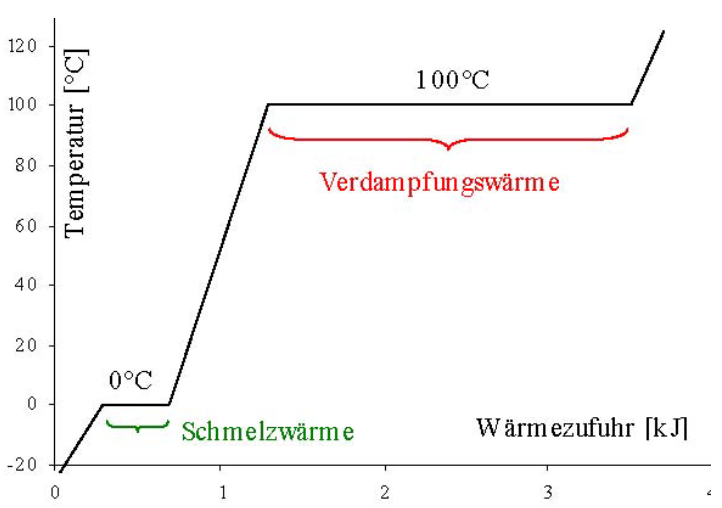
\includegraphics[width=0.99\linewidth]{Bilder/latente_waerme_2}\\
\\
\end{minipage}
\hfill
\begin{minipage}{0.5\linewidth}
Beim Schmelzen und Verdampfen findet \textbf{keine} Temperaturerhöhung statt \\
Beim Gefrieren und oder \\
Kondensieren wird diese \\
versteckte Wärme wieder frei, \textbf{ohne} Abnahme der Temperatur \\
\\
\end{minipage}

\textbf{Die Schmelz-/ Verdampfungswärme ist stark druckabhängig} \\


$$ \boxed{ Q_f = q_f \cdot m } \qquad \qquad q_{f_{Wasser}} := 334 \mathrm{\frac{kJ}{kg}} $$

$$ \boxed{ Q_s = q_s \cdot m } \qquad \qquad q_{s_{Wasser}} := 2256 \mathrm{\frac{kJ}{kg} } $$



\begin{tabular}{c l c}

	$Q_f$ & Schmelz-/Erstarrungs-Wärme & $[Q_f] = \mathrm{J}$ \\
	\rule{0pt}{8pt}$q_f$ & Spezifische Schmelzwärme & $[q_f] = \mathrm{\frac{J}{kg}}$ \\
	$Q_S$ & Verdampfungs-/Kondensations-Wärme & $[Q_S] = \mathrm{J}$ \\
	\rule{0pt}{8pt}$q_s$ & Spezifische Verdampfungs-Wärme& $[q_s] = \mathrm{\frac{J}{kg}}$ \\
	$m$ & Masse & $[m] = \mathrm{kg}$ \\
\end{tabular}




% \vfill\null
% \columnbreak



\subsection{Wärmebilanz}
Wärmeaustausch zwischen verschiedenen Materialien \\

In einem abgeschlossenen System (nach aussen isoliert) muss gelten: \\
\textbf{Zugeführte Wärme = Abgeführte Wärme}

$$  \boxed{ \sum_{i=1}^n  ( \Delta Q_i + \Delta Q_{f_i} + \Delta Q_{s_i} ) = 0 } $$


\begin{tabular}{c l c}
	$\Delta Q_i$ & i-te Wärme-Menge aus & $[\Delta Q_i] = \mathrm{J}$ \\
				& Temperatur-Zu-/Abnahme & \\
	$\Delta Q_{f_i}$ & i-te Wärme-Menge aus  &  $[\Delta Q_{f_i}] = \mathrm{J}$ \\
				& Schmelz-/Erstarrungs-Vorgang  & \\
	$\Delta Q_{s_i}$ & i-te Wärme-Menge aus & $[\Delta Q_{s_i}] = \mathrm{J}$\\
					 & Verdampfungs-/Kondensations-Vorgang &  \\
	& +  zugeführte Wärme-Menge &  \\
	& - abgeführter Wärme-Menge & \\
\end{tabular}




\section{Phasen und Phasenübergänge}


\subsection{Phasen}


\begin{tabular}{ll}
$\bullet$ & \textbf{Fest} \\
		  & feste Gestalt; festes Volumen \\
$\bullet$ & \textbf{Flüssig} \\
		  & keine feste Gestalt; festes Volumen \\
$\bullet$ & \textbf{Gasförmig} \\
		  & keine feste Gesalt; kein festes Volumen \\
$\bullet$ & \textbf{Plasma} \\
		  & Bei sehr hoher Temperatur ist Materie ionisiert (Elektronengas) \\
$\bullet$ & \textbf{Mischung / Dispersion:} \\
\end{tabular}

\begin{center}
	\begin{tabular}{l|cc}
		                   & \textbf{flüssig} & \textbf{gasförmig} \\ \hline
		\textbf{fest}      & Suspension (Sol) & Aerosol (Rauch) \\
		\textbf{flüssig}   & Emulsion & Aerosol (Nebel) \\
		\textbf{gasförmig} & Schaum & - \\
	\end{tabular}
\end{center}

%\subsection{Zweiphasengebiete (pT-Diagramm}



% \vfill\null
% \columnbreak


\subsection{Dampfdruck $p_s(T)$}
\textbf{Der Dampfdruck bedeutet das Gleichgewicht der Flüssigkeit mit ihrer Dampfphase} \\

Der Dampfdruck ist das Niveau des kontanten Drucks im\\
2-Phasengebiet eines realen Gases nach van der Waals. \\
\\
Der Dampfdruck ist nur \textbf{temperaturabhängig} \\
\\
Bei Kompression oder Expansion ändert sich der Dampfdruck nicht, sondern der Anteil Flüssigkeit zu Gas muss ändern \\
\\

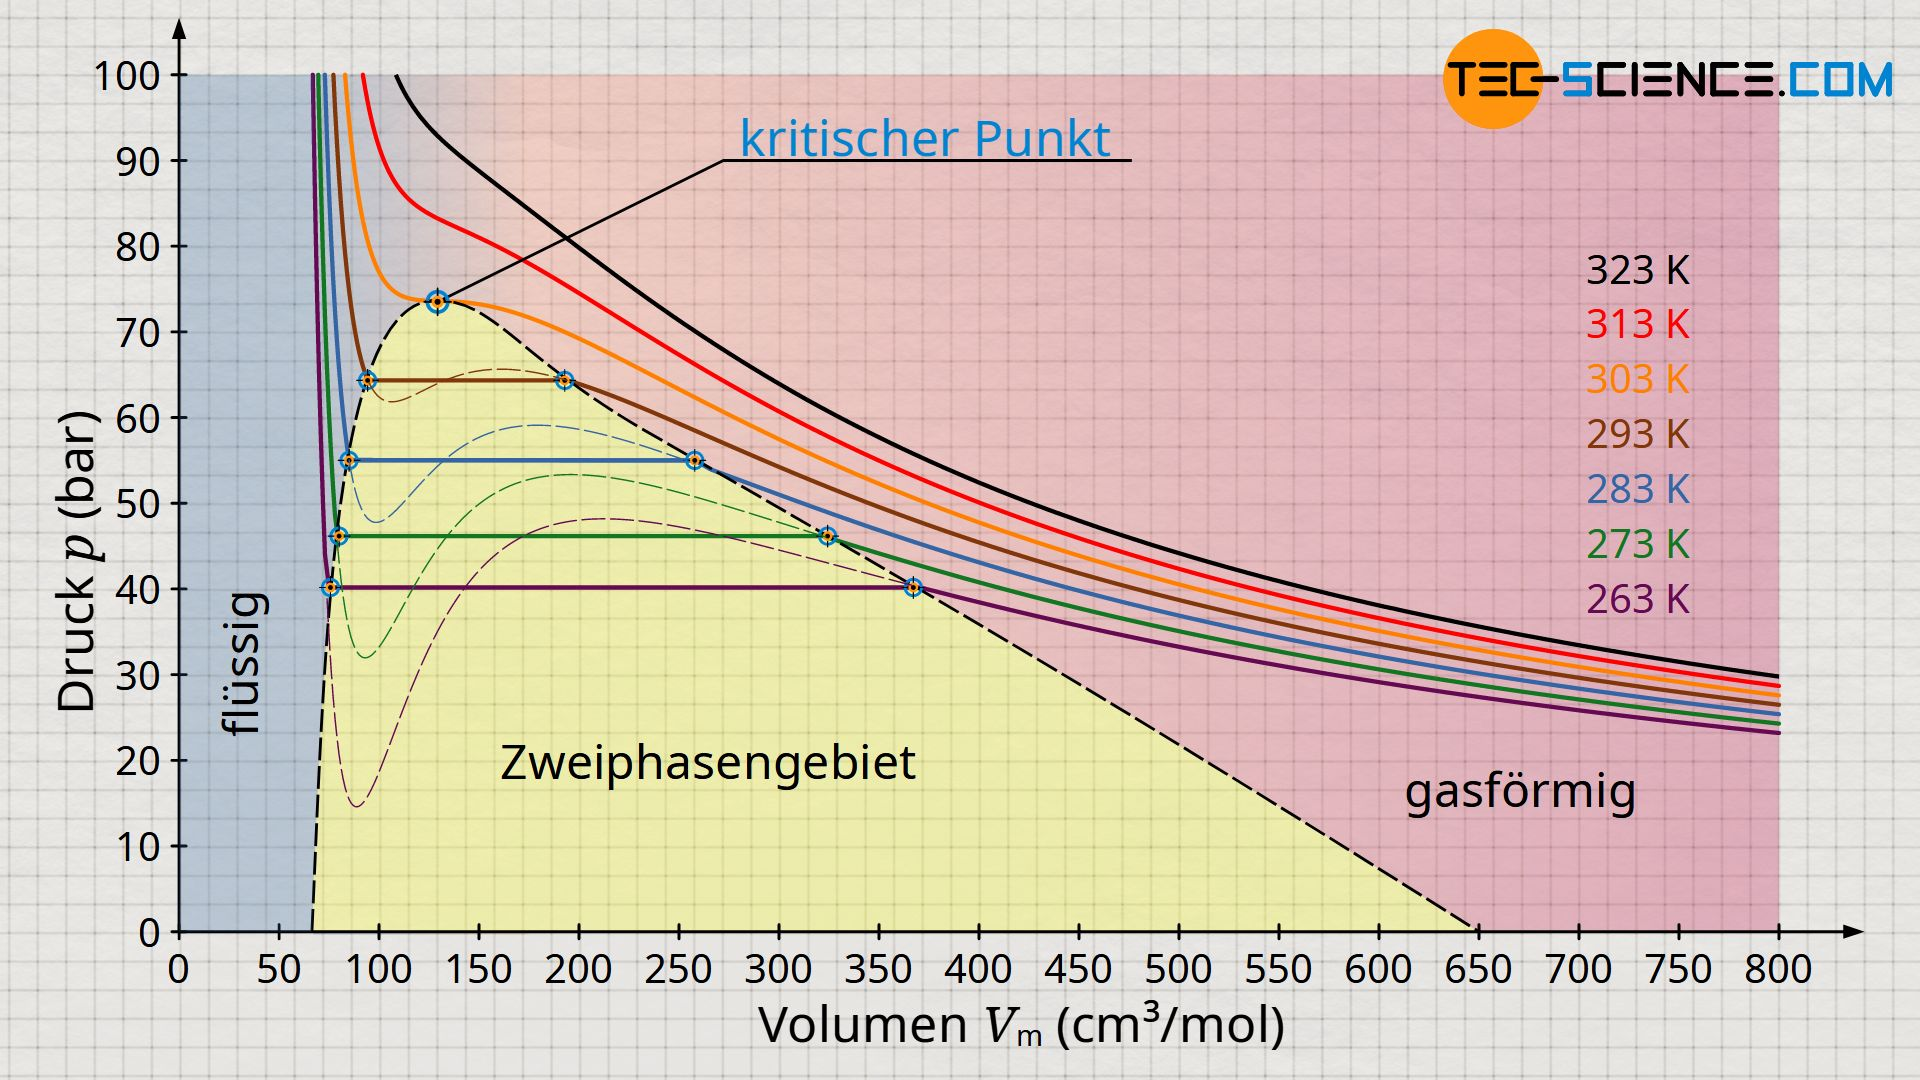
\includegraphics[width=0.9\linewidth]{Bilder/dampfdruck} \\
\\
\textbf{Verdunsten} $\Rightarrow$ Schnellste Teilchen treten aus Flüssigkeit aus \\
\\
\textbf{Sieden/Verdampfen} Dampfdruck = Umgebungsdruck



\vfill\null
\columnbreak



\subsection{Dampfdruck-Kurve (Clausius-Clapeyron)}

\textbf{Kondensieren $\Leftrightarrow$ Verdampfen}  \qquad flüssig $\Leftrightarrow$ gasförmig  \\

$$ \boxed{ \frac{d \, p_s}{d\, T} = \frac{q_s}{T \cdot  \Big( \frac{1}{\rho_g} - \frac{1}{\rho_f} \Big)  }     } $$



\subsubsection{Dampfdruck $p_s(T)$ von Wasser (Clausius-Clapeyron)}

$$ \boxed{ p_s(T) = p_{s0} \cdot e^{\frac{q_s \cdot M_W}{R} \cdot ( \frac{1}{T_0} - \frac{1}{T}) } } $$

$$ p_{s0} = 610.7 \, \mathrm{Pa} \quad T_0 = 273 \, \mathrm{K} \quad q_s = 2420 \, \mathrm{\frac{kJ}{kg}} \quad M_W = 18.02 \, \mathrm{\frac{g}{mol}}  $$



\subsection{Schmelzdruck-Kurve (Clausius-Clapeyron)}

\textbf{Erstarren $\Leftrightarrow$ Schmelzen}  \qquad fest $\Leftrightarrow$ flüssig \\

$$ \boxed{ \frac{d \, p_f}{d\, T} = \frac{q_f}{T \cdot  \Big( \frac{1}{p_f} - \frac{1}{p_s} \Big)  }     } $$




\subsection{Gasdruck-Kurve (Clausius-Clapeyron)}

\textbf{Desublimieren $\Leftrightarrow$ Sublimieren} \qquad fest $\Leftrightarrow$ gasförmig \\

$$ \boxed{ \frac{d \, p_{sub}}{d\, T} = \frac{q_s + q_f}{T \cdot  \Big( \frac{1}{\rho_g} - \frac{1}{\rho_s} \Big)  }     } $$



\begin{tabular}{c l c}
	\rule{0pt}{10pt}$q_s$ & spezifische Verdampfungs-Wärme & $[q_s] = \mathrm{\frac{J}{kg}}$ \\
	\rule{0pt}{10pt}$q_f$ & spezifische Schmelz-Wärme & $[q_f] = \mathrm{\frac{J}{kg}}$ \\
	$q_s + q_f$ & spezifische Sublimations-Wärme & \\
	$p_s$ & Dampfdruck & $[p_s] = \mathrm{Pa}$ \\
	$p_f$ & Schmelzdruck & $[p_f] = \mathrm{Pa}$ \\
	$p_g$ & Schmelzdruck & $[p_g] = \mathrm{Pa}$ \\
	\rule{0pt}{10pt}$\rho_g$ & Dichte Gas & $[\rho_g] = \mathrm{\frac{kg}{m^3}}$ \\
	\rule{0pt}{10pt}$\rho_f$ & Dichte Flüssgkeit & $[\rho_f] = \mathrm{\frac{kg}{m^3}}$ \\
	\rule{0pt}{10pt}$\rho_s$ & Dichte Festkörper & $[\rho_s] = \mathrm{\frac{kg}{m^3}}$ \\
	$T$ & Temperatur   & $[T] = K$ \\
	$M$ & Molare Masse & $[M] = \frac{kg}{mol}$ \\
	\rule{0pt}{8pt}$R$ & Universelle Gaskonstante: $R = 8.314 \mathrm{\frac{J}{mol \cdot K}}$ & $[R] = \mathrm{\frac{J}{mol \cdot K}} $ \\
\end{tabular}


% \vfill\null
% \columnbreak



\subsection{Formeln von Magnus}
Die Formeln von Magnus dienen der vereinfachten Berechnung des Dampfdrucks von Wasser = Sättigungsdruck 

\subsubsection{Dampfdruck von Wasser $p_s(\theta)$ $(\theta \geq 0 ^{\circ}C)$}


$$ \boxed{ p_s(\theta) = p_{s0} \cdot 10^{ \frac{7.5 \cdot \theta}{\theta + 237}  } } $$



\subsubsection{Schmelzdruck von Wasser $p_s(\theta)$ $ (\theta \leq 0 ^{\circ}C)$}

$$ \boxed{ p_s(\theta) = p_{s0} \cdot 10^{ \frac{9.5 \cdot \theta}{\theta + 265.5} } } $$


\subsubsection{WMO erweiterte Lösung $p_s(\theta)$ $ (-40^{\circ}C < \theta < 50^{\circ}C) $}

$$ \boxed{p_s(\theta) = p_{s0} \cdot \e ^{\left( \frac{17.62 \cdot \theta}{243.04 + \theta} \right)} }$$



\begin{tabular}{c l c}
	$p_s$ & Dampfdruck / Schmelzdruck & $[p_s] = \mathrm{Pa}$ \\
	$p_{s0}$ & Dampfdruck bei $0^{\circ}C$ \quad $p_{s0} = 610.7 \mathrm{Pa} $ & $[p_{s0}] = \mathrm{Pa}$ \\
	$\theta$ & Temperatur & $[\theta] = \text{°C}$ \\
	
\end{tabular}




\subsection{Umkehrformeln von Magnus}

\subsubsection{$\theta(p_s)$ für $p_s \geq p_{s0}$}


$$ \boxed{ \theta(p_s) = \frac{237 \cdot log \big( \frac{p_s}{6.107} \big)  }{7.5 - log \big( \frac{p_s}{6.107} \big)} } $$



\subsubsection{$\theta(p_s)$ für $p_s \leq p_{s0}$}

$$ \boxed{ \theta(p_s) = \frac{265.5 \cdot log \big( \frac{p_s}{p_{s0}} \big)  }{9.5 - log \big( \frac{p_s}{p_{s0}} \big)} } $$




\subsection{Luftfeuchtigkeit}

\subsubsection{Absolute Luftfeuchtigkeit  $f$}

$$ \boxed{ f = \frac{m_W}{V}  } $$



\subsubsection{Relative Luftfeuchtigkeit $f_r$}

$$ \boxed{ f_r = \frac{m_W}{m_S} = \frac{p_D}{p_S} = \frac{p_D}{p_S(\theta)}  } $$



\begin{tabular}{c l c}
	$f$ & Absolute Luftfeuchtigkeit & $[f] = \frac{kg}{m^3}$ \\
	$f_r$ & Relative Luftfeuchtigkeit & $[f_r] = 1$ \\
	$m_W$ & Masse Wasserdampf & $[m_W] = \mathrm{kg}$ \\
	$m_S$ & Masse Wasserdampf bei Sättigung & $[m_S] = \mathrm{kg}$ \\
	$V$ & Volumen & $[V] = \mathrm{m^3}$ \\
	$p_D$ & Partialdruck Wasserdampf & $[p_D] = \mathrm{Pa}$ \\
	$p_S$ & Dampfdruck = Sättigungsdruck Wasserdampf & $[p_s] = \mathrm{Pa}$ \\
	$\theta$ & Temperatur & $[\theta] = \text{°C}$ \\
\end{tabular}


% \vfill\null
% \columnbreak



\subsubsection{Feuchte vs. trockene Luft}

\textbf{Feuchte Luft ist leichter als trockene Luft!}

% $$ \boxed{ \rho_f < \rho_t } \qquad \mathrm{(da} \, M_W < M_L \mathrm{)}$$

$$ \boxed{ \rho_f = \rho_t + \frac{p_D}{RT}(M_W - M_L)} $$

\begin{tabular}{c l c}
	\rule{0pt}{10pt}$\rho_f$ & Dichte feuchte Luft & $[\rho_f] = \mathrm{\frac{kg}{m^3}}$ \\
	\rule{0pt}{10pt}$\rho_t$ & Dichte trockene Luft & $[\rho_t] = \mathrm{\frac{kg}{m^3}}$ \\
	\rule{0pt}{10pt}$p_D$ & Partialdruck Wasserdampf & $[p_D] = \mathrm{Pa}$ \\
	\rule{0pt}{10pt}$T$   & Temperatur & $[T] = K$ \\
	\rule{0pt}{10pt}$M_W$ & Molmasse $H_2O$ & $[M_W] = \mathrm{\frac{kg}{mol}}$ \\
	\rule{0pt}{10pt}$M_S$ & Molmasse Luft g & $[M_W] = \mathrm{\frac{g}{mol}}$ \\
	\rule{0pt}{10pt}$R$ & Universelle Gaskonstante: $R = 8.314 \mathrm{\frac{J}{mol \cdot K}}$ & $[R] = \mathrm{\frac{J}{mol \cdot K}} $ \\	
\end{tabular}



\subsection{Taupunkts-Temperatur $\theta_d$}
Temperatur, bei welcher 100\% Luftfeuchtigkeit herrscht. \\
\\
Wenn die Taupunkt-Temperatur \textbf{unterschritten} wird, dann \\
kondensiert Wasser.

$$ \boxed{ \theta_d (\theta, f_r) = \frac{237 \cdot \Big( \log(f_r) + \frac{7.5 \cdot \theta}{\theta + 237}    \Big)}{7.5 - \Big( \log(f_r) + \frac{7.5 \cdot \theta }{\theta + 237} \Big) }  }$$


$$ \boxed{ \theta_d (x) = \frac{237 \cdot x}{7.5 - x}    \qquad  \text{mit } \quad    x(\theta, f_r) = \log(f_r) + \frac{7.5 \cdot \theta}{\theta + 237}  }   $$


\begin{tabular}{c l c}
	$\theta_d$ & Taupunkts-Temperatur & $[\theta_d] = \text{°C}$ \\
	$f_r$ & relative Luftfeuchtigkeit & $[f_r] = 1$ \\
	$\theta$ & Temperatur & $[\theta] = \text{°C}$ \\
\end{tabular}




\subsection{Relative Innen-Feuchte $f_{ri}$}

$$ \boxed{ f_{ri} = \frac{p_s(\theta_a)}{p_s(\theta_i)} \cdot f_{ra}  }$$

\begin{tabular}{c l c}
	$f_{ri}$ & relative Feuchte im Inneren & $[f_{ri}] = 1$ \\
	$f_{ra}$ & relative Feuchte der Aussenluft & $[f_{ra}] = \text{1}$ \\
	$p_s(\theta_i)$ & Dampfdruck bei Innentemperatur & $[p_s(\theta_i)] = \mathrm{Pa}$ \\
	$p_s(\theta_a)$ & Dampfdruck bei Aussentemperatur &  $[p_s(\theta_a)] = \mathrm{Pa}$  \\
\end{tabular}



% \vfill\null
% \columnbreak


\section{Kinetische Gas-Theorie} %TODO: Evtl. Folie 6, Seite 5 noch einf¨ügen 

\subsection{Aequipartitionsgesetz}

\textbf{Mittlere kinetische Energie} \\
\\
Idealisierte Annahmen: \\

\begin{tabular}{ll}
1. & Moleküle = Massenpunkte \\
2. & Keine (bzw.) elastische Zusammenstösse \\
3. & Keine Kräfte zwischen den Molekülen\\
4. & Elastischer Stoss gegen Wand \\
5. & Alle Moleküle haben gleiche Geschwindigkeit \\
6. & 1/6 aller Moleküle fliegen gegen eine einzelne Wand \\
\\
\end{tabular}


\begin{minipage}{0.48\linewidth}
$$ \boxed{ \overline{E} = f \cdot \frac{k \cdot T}{2} } $$
\end{minipage}
\hfill
\begin{minipage}{0.48\linewidth}
\begin{tabular}{ll}
f = 3 & 1-atomiges Gas \\
f = 5 & 2-atomiges Gas \\
f = 6 & 3-atomiges Gas \\
\\
\end{tabular}
\end{minipage}


\begin{tabular}{c l c}
	$\overline{E}$ & Mittlere kinetische Energie & $[\overline{E}] = \mathrm{J}$ \\
	$f$ & Freiheitsgrade & $[f] = \text{1}$ \\
	\rule{0pt}{8pt}$k$ & Boltzmann-Konstante $k = 1.381 \cdot 10^{-23} \mathrm{\frac{J}{K}}$ & $[k] = \mathrm{\frac{J}{K}}$ \\
	$T$ & \textbf{Absolute} Temperatur & $[T] = \mathrm{K}$ \\	
\end{tabular}


\subsection{Geschwindigkeiten}

\subsubsection{Mittlere quadratische Geschwindigkeit  $u$}

$$ \boxed{ u = \sqrt{\frac{3 \cdot k \cdot T}{m}} = \sqrt{\frac{3 \cdot R \cdot T}{M}} }  $$


\subsubsection{Mittlere Geschwindigkeit $\overline{v}$}

$$ \boxed{ \overline{v} = \sqrt{\frac{8 \cdot k \cdot T}{\pi m}} = \sqrt{\frac{8 \cdot R \cdot T}{\pi M}} }  $$


\subsubsection{Wahrscheinlichste Geschwindigkeit $v_0$}

$$ \boxed{ v_0 = \sqrt{\frac{2 \cdot k \cdot T}{m}} = \sqrt{\frac{2 \cdot R \cdot T}{M}}  }  $$




\begin{tabular}{c l c}
	\rule{0pt}{8pt}$k$ & Boltzmann-Konstante $k = 1.381 \cdot 10^{-23} \mathrm{\frac{J}{K}}$ & $[k] = \mathrm{\frac{J}{K}}$ \\
	$T$ & \textbf{absolute} Temperatur & $[T] = \mathrm{K}$ \\
	$m$ & Masse des Teilchens & $[m] = \mathrm{kg}$ \\
	$M$ & Molmasse & $[M] = \frac{kg}{mol}$ \\
	\rule{0pt}{10pt}$R$ & Universelle Gaskonstante: $R = 8.314 \mathrm{\frac{J}{mol \cdot K}}$ & $[R] = \mathrm{\frac{J}{mol \cdot K}} $ \\	
\end{tabular}




\subsection{Maxwell-Boltzmann-Verteilung}

$$ \boxed{ f(m, \, T, \, v) = \sqrt{\frac{2 \cdot m^3}{\pi \cdot k^3 \cdot T^3 }}  \cdot v^2 \cdot \e ^{- \frac{m \cdot v^2}{2 \cdot k \cdot T}}  }  $$


\begin{tabular}{c l c}
	$m$ & Masse des Teilchens & $[m] = \mathrm{kg}$ \\
	\rule{0pt}{8pt}$k$ & Boltzmann-Konstante $k = 1.381 \cdot 10^{-23} \mathrm{\frac{J}{K}}$ & $[k] = \mathrm{\frac{J}{K}}$ \\
	$T$ & \textbf{absolute} Temperatur & $[T] = \mathrm{K}$ \\
	\rule{0pt}{8pt}$v$ & Geschwindigkeit & $[v] = \mathrm{\frac{m}{s}}$ \\
\end{tabular}





\subsection{Mittlere freie Weglänge $\overline{\lambda}$}

Gibt an, um welche Strecke sich ein Molekül im Mittel bis zum nächsten Zusammenstoss fortbewegen kann.

$$ \boxed{ \overline{\lambda} = \frac{1}{\sqrt{2}} \cdot \frac{1}{n \cdot (\pi \cdot d^2 )} }  \qquad \text{mit Wirkungsquerschnitt } \sigma = \pi \cdot d^2$$

\begin{tabular}{c l c}
	\rule{0pt}{8pt}$n$ & \textcolor{red}{Molekül-Dichte} & $[n] = \mathrm{\frac{1}{m^3}}$\\	
	$d$ & Molekül-Durchmesser & $[d] = \mathrm{m}$ \\
\end{tabular}




\subsection{Dichtefunktion}
Verteilungsfunktion der mittleren, freien Weglänge 

$$ \boxed{ f(x) = \frac{1}{\overline{\lambda}} \cdot \e^{- \frac{x}{\overline{\lambda}}}  } $$


\subsection{Transportvorgänge}

\subsubsection{Wärmeleitung}
Transport von \textbf{kinetischer Energie} (als Wärme wahrgenommen)

$$ \boxed{ j_Q = - \lambda_Q \cdot \frac{\mathrm{dT}}{\mathrm{dx}} \qquad \quad \lambda_Q = \frac{1}{6} \cdot n \cdot \overline{v} \cdot \overline{\lambda} \cdot f \cdot k }  $$




\subsubsection{Diffusion}
Transport von \textbf{Masse} 


$$ \boxed{ j_D = -D \cdot \frac{\mathrm{dn}}{\mathrm{dx}} \qquad \quad  D = \frac{1}{3} \cdot \overline{v} \cdot \overline{\lambda} }  $$



\subsubsection{Viskosität ($v << v_{therm}$)}
Transport von \textbf{Impuls} 


$$ \boxed{ \tau = - \eta \cdot \frac{\mathrm{dv}}{\mathrm{dx}} \qquad \quad  \eta = \frac{1}{3} \cdot \overline{v} \cdot \overline{\lambda} \cdot \rho }  $$


\begin{tabular}{c l c}
	\rule{0pt}{10pt}$j_Q$ & Wärmestrom & $[j_Q] = \mathrm{\frac{W}{m^2}}$ \\
	\rule{0pt}{10pt}$\lambda_Q$ & Wärmeleitfähigkeit & $[\lambda_Q] = \mathrm{\frac{W}{m \cdot K}}$ \\
	$j_D$ & Diffusionsstrom & $[j_D] = ?$ \\
	\rule{0pt}{10pt}$D$ & Diffusionskonstante & $[D] = \mathrm{\frac{m^2}{s}}$ \\
	$\tau$ & Schubspannung & $[\tau] = \mathrm{N}$ \\
	$\eta$ & Viskosität & $[\eta] = \mathrm{Pa \cdot s}$ \\
	\rule{0pt}{10pt}$n$ & \textcolor{red}{Molekül-Dichte} & $[n] = \mathrm{\frac{1}{m^3}}$\\	
	\rule{0pt}{10pt}$\overline{v}$ & Mittlere Geschwindigkeit & $[\overline{v}] = \mathrm{\frac{m}{s}}$ \\
	\rule{0pt}{10pt}$\overline{\lambda}$ & Mittlere freie Weglänge & $[\overline{\lambda}] = \mathrm{m}$ \\
	$f$ & Anzahl Freiheitsgrade & $[f] = \mathrm{1}$ \\
	\rule{0pt}{10pt}$k$ & Boltzmann-Konstante $k = 1.381 \cdot 10^{-23} \mathrm{\frac{J}{K}}$ & $[k] = \mathrm{\frac{J}{K}}$ \\
	$T$ & \textbf{absolute} Temperatur & $[T] = \mathrm{K}$ \\
	\rule{0pt}{10pt}$\rho$ & Dichte & $[\rho] = \mathrm{\frac{kg}{m^3}}$ \\
\end{tabular}


\section{Temperaturstrahlung}

\begin{tabular}{ll}
$\bullet$ & Wärmestahlung = Berührungslose Übertragung von Wärme \\
$\bullet$ & In Form von elektromagnetischen Wellen ($\lambda$ @ IR) \\
$\bullet$ & Körper absorbiert elektromagn. Strahlung und erhöht \\
		  & seine Temperatur \\ 
          & Jeder Körper mit $T > 0 \, K$ straht Wärme ab (Temp-strahlung) \\
$\bullet$ & Für jede Wellenlänge muss ein Körper gleich viel  \\
		  & Energie abstahlen, wie er zuvor aufgenommen hat!\\
\end{tabular}




\subsection{Strahlungs-Gesetze}


\subsubsection{Stefan-Boltzmann-Gesetz}

\begin{tabular}{ll}
$\bullet$ & Ideal schwarzer Körper (Hohlraum) absoliert  \\
		  & \textbf{alle Wellenlängen zu 100 \%}   \\		
$\bullet$ & Je mehr ein Körper absorbiert, desto mehr muss er \\
		  & emmitieren \textbf{(Energie-Gleichgewicht)}   \\	
		  \\
\end{tabular}

Ein schwarzer Körper (=Hohlraumstrahler) der Temperatur $T$ hat eine totale Abstrahlungs-Leistung \textbf{pro Oberfläche} $K_S$ von: 

$$ \boxed{ K_S = \sigma \cdot T^4 }  $$



\begin{tabular}{c l c}
	\rule{0pt}{10pt}$K_S$ & Schwarzkörper-Emission & $[K_S] = \mathrm{\frac{W}{m^2}}$ \\
	\rule{0pt}{10pt}$\sigma$ & Stefan-Boltzmann-Konstante  & $[\sigma] = \mathrm{\frac{W}{m^2 \cdot K^4}}$\\
	\rule{0pt}{10pt}&  $\sigma = 5.671 \cdot 10^{-8} \, \mathrm{\frac{W}{m^2 \cdot K^4}}$ &  \\ \\
	$T$ & Temperatur & $[T] = \mathrm{K}$ \\
\end{tabular}




\subsubsection{Wien'sches Verschiebungsgesetz}

Verschiebung der maximalen Wellenlänge:

$$ \boxed{ \lambda_{max} \cdot T = \const = b  }  $$

\begin{tabular}{c l c}
	$\lambda_{max}$ & Wellenlängen-Maximum (Planck) & $[\lambda_{max}] = \mathrm{m}$ \\
	$T$ & Temperatur & $[T] = \mathrm{K}$ \\
	\rule{0pt}{8pt}$b$ & Konstante: $b = 2.898 \cdot 10^{-3} \mathrm{ m \cdot K}$ & $ [b] = \mathrm{ m \cdot K}$ \\
\end{tabular}





\subsubsection{Planck'sches Gesetz der Quantenmechanik}

Ein Oszillator, welcher auf ein anderes Energieniveau  \\
(=Elektronen-Kreisbahnen nach Bohr) wechselt, setzt die \\
Energiedifferenz $\Delta E$ in ein Lichtquant (Photon) mit \\
entsprechender Frequenz $f$ um. \\
Je nach Vorzeichen von $\Delta E$ wird das Photon emmitiert  \\
oder absorbiert . \\

$$ \boxed { \Delta E = h \cdot f }  $$

\begin{tabular}{c l c}
	$\Delta E$ & spektrale Abstrahlung (Energie) & $[\Delta E] = \mathrm{J}$ \\
	$h$ & Planck'sches Wirkungsquantum & $[h] = \mathrm{J \cdot s} $\\
	&  $h = 6.628 \cdot 10^{-34} \, \mathrm{J \cdot s}$ &  \\
	\rule{0pt}{8pt}$f$ & Frequenz des Photons & $ [f] = \mathrm{\frac{1}{s} = Hz}$ \\
\end{tabular}



% \vfill\null
% \columnbreak


\subsection{Wärmetransport (an Beispiel Hauswand)}


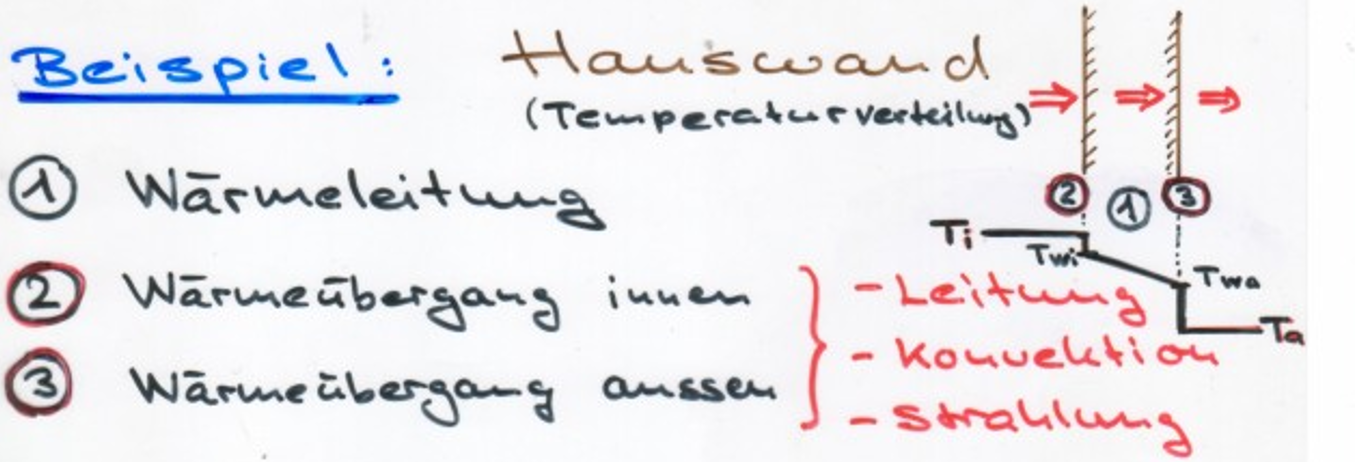
\includegraphics[width=0.9\linewidth]{Bilder/Waermetransport} \\


\subsubsection{Wärmeleitung}

$$ \boxed{ j = - \lambda \cdot \frac{\mathrm{d} T}{\mathrm{d} x}  } $$ 


\begin{tabular}{c l c}
	\rule{0pt}{10pt}$j$ & Wärmestromdiche & $[j] = \mathrm{\frac{W}{m^2}}$ \\
	\rule{0pt}{10pt}$\lambda$ & Wärmeleitfähigkeit & $[\lambda] = \mathrm{\frac{W}{m \cdot K}} $\\
	\rule{0pt}{10pt}$\frac{\mathrm{d} T}{\mathrm{d} x}$ & Wärmeabnahme / Gradient & $ [\frac{\mathrm{d} T}{\mathrm{d} x}] = \mathrm{\frac{T}{m}}$ \\
\end{tabular}


\subsubsection{Wärmeübergang}

$$ \boxed{\mathrm{innen:} \quad  j = \alpha_i \cdot (T_i - T_{wi} )  \qquad \mathrm{mit} \, \alpha_i = 8 \mathrm{\frac{W}{m^2 \cdot K}}  }  $$ 

$$ \boxed{\mathrm{aussen:} \quad  j = \alpha_a \cdot (T_{wa} - T_a )  \qquad \mathrm{mit} \, \alpha_a = 20 \mathrm{\frac{W}{m^2 \cdot K}}  }  $$ 





\subsubsection{Wärmedurchgang}
Material + Dicke zusammengefasst

$$ \boxed{ j = k \cdot (T_i - T_a) = k \cdot \Delta T  \qquad \mathrm{mit} \, k = \frac{\lambda}{d} }  $$ 



\begin{tabular}{c l c}
	\rule{0pt}{10pt}$j$ & Wärmestromdiche & $[j] = \mathrm{\frac{W}{m^2}}$ \\
	\rule{0pt}{10pt}$\lambda$ & Wärmeleitfähigkeit & $[\lambda] = \mathrm{\frac{W}{m \cdot K}} $\\
	\rule{0pt}{10pt}$\frac{\mathrm{d} T}{\mathrm{d} x}$ & Wärmeabnahme / Gradient & $ [\frac{\mathrm{d} T}{\mathrm{d} x}] = \mathrm{\frac{T}{m}}$ \\
	\rule{0pt}{10pt}$\alpha_i$ & Wärmeübergangszahl innen & $[\alpha_i] = \mathrm{\frac{W}{m^2 \cdot K}} $\\
	\rule{0pt}{10pt}$\alpha_a$ & Wärmeübergangszahl aussen & $[\alpha_a] = \mathrm{\frac{W}{m^2 \cdot K}} $\\
	$T_{wa}$ & Temperatur Wand aussen & $[T_{wa}] = \mathrm{K}$ \\
	$T_a$ & Aussentemperatur & $[T_a] = \mathrm{K}$ \\
	$T_{wi}$ & Temperatur Wand innen & $[T_{wi}] = \mathrm{K}$ \\
	$T_i$ & Innentemperatur & $[T_i] = \mathrm{K}$ \\
	\rule{0pt}{10pt}$k$ & Wärmedurchgangszahl & $[k] = \mathrm{\frac{W}{m^2 \cdot K}}$ \\
	$d$ & Dicke der Wand & $[d] = \mathrm{m}$ \\
	\\
\end{tabular}


$$ \textcolor{orange}{  \boxed{ P =  \dot{Q} = j \cdot A } } $$ 




% \vfill\null
% \columnbreak



\subsubsection{Wärmedurchgang komplett}

Der komplette Wärmedurchgang leitet sich her durch die \textbf{Erhaltung der Wärmestrondichte $j$} und errechnet sich mit:

% $$ \boxed{\mathrm{2 \; Schichten:} \quad \frac{1}{k_{12}} = \frac{1}{k_1} + \frac{1}{k_2} }  $$  

$$ \boxed{\mathrm{n \; Schichten:} \quad \frac{1}{k_{tot}} = \frac{1}{\alpha_i} + \sum_x  \frac{1}{k_x} + \frac{1}{\alpha_a}  }  $$

$$ \boxed{\mathrm{zylindrisch:} \quad \frac{1}{k_{tot}} = r_a \Big(  \frac{1}{\alpha_i \cdot r_i} + \sum_x \frac{1}{\lambda_x} \cdot \ln \big( \frac{r_{xa}}{r_{xi}} \big)  + \frac{1}{\alpha_a \cdot r_a} \Big) }  $$




\begin{tabular}{c l c}
	\rule{0pt}{10pt}$k_x$ & Wärmedurchgangszahl x-te Schicht & $[k_x] = \mathrm{\frac{W}{m^2 \cdot K}}$ \\
	\rule{0pt}{10pt}$\alpha_i$ & Wärmeübergangszahl innen & $[\alpha_i] = \mathrm{\frac{W}{m^2 \cdot K}} $\\
	\rule{0pt}{10pt}$\alpha_a$ & Wärmeübergangszahl aussen & $[\alpha_a] = \mathrm{\frac{W}{m^2 \cdot K}} $\\
	$r_i$ & Innenradius Rohr & $[r_i] = \mathrm{m}$	 \\
	$r_a$ & Aussenradius Rohr & $[r_a] = \mathrm{m}$	 \\
	\rule{0pt}{10pt}$\lambda_x$ & Wärmeleitfähigkeit & $[\lambda] = \mathrm{\frac{W}{m \cdot K}} $\\
\end{tabular}





\subsection{Wärme-Bedarf (Heizleistung)}
Der Wärme-Bedarf (=Heizleistung) setzt sich zusammen aus \textbf{Wärmeverlust durch Wärmeleitung} und durch \textbf{Wärmeverlust durch Luftaustausch}: 

$$\mathrm{\underbrace{W"armeverlust}_{\substack{\dot{Q}}}  = \underbrace{Heizleistung}_{\substack{P}}  }   $$

$$ \boxed{ P = \dot{Q}_{tot} = \dot{Q}_W + \dot{Q}_L }   $$

\begin{minipage}{0.46\linewidth}
$$ \boxed{ \dot{Q}_W = A \cdot j = A \cdot k \cdot \Delta T  }$$ \\
\end{minipage}
\hfill
\begin{minipage}{0.46\linewidth}
$$ \boxed{ \dot{Q}_L = c_L \cdot \rho_L \cdot \dot{V} \cdot \Delta T}   $$
\\
\end{minipage}



$$ \boxed{ \mathrm{allgemein: } \quad \dot{Q}_{tot} = \sum_{i=1}^n  \big[  (A_i \cdot k_i + c_L \cdot \rho_L \cdot \dot{V} ) \cdot \Delta T \big]  }   $$


\begin{tabular}{c l c}
	\rule{0pt}{10pt}$\dot{Q}_{tot}$ & Totaler Wärmeverlust & $[\dot{Q}_{tot}] = \mathrm{\frac{J}{s} = W}$ \\
	\rule{0pt}{10pt}$\dot{Q}_W$ & Wärmeleitung & $[\dot{Q}_W] = \mathrm{\frac{J}{s} = W}$ \\
	\rule{0pt}{10pt}$\dot{Q}_L$ & Luftaustausch & $[\dot{Q}_L] = \mathrm{\frac{J}{s} = W}$ \\
	\rule{0pt}{10pt}$k_i$ & Wärmedurchgangszahl i-te Schicht & $[k_i] = \mathrm{\frac{W}{m^2 \cdot K}}$ \\
	\rule{0pt}{10pt}$\dot{V}$ & Volumenstrom & $[\dot{V}] = \mathrm{\frac{m^3}{s}}$ \\
	\rule{0pt}{10pt}$\rho_L$ & Dichte der Luft: $\rho_L = 1.2 \, \mathrm{\frac{kg}{m^3}}$ & $[\rho_L] = \mathrm{\frac{kg}{m^3}}$ \\
	\rule{0pt}{10pt}$c_L$ & Wärmekapazität Luft: $c_L = 1000 \, \mathrm{\frac{J}{kg \cdot K}}$ & $[c_L] = \mathrm{\frac{J}{kg \cdot K}}$ \\
	$A$ & Fläche der Wärmeleitung & $[A] = \mathrm{m^2}$ \\
	$\Delta T$ & Temperaturdifferenz & $[\Delta T] = \mathrm{K}$ \\
\end{tabular}



% \vfill\null
% \columnbreak



\subsection{Wärmeverlust durch Abstrahlung}

Durch Strahlung kann auch Wärme übertragen werden.

$$ \boxed{ j_{12} = c_{12} \cdot (T_1^4 - T_2^4) = \sigma \cdot \varepsilon \cdot (T_1^4 - T_2^4) }   $$



\begin{tabular}{c l c}
	\rule{0pt}{10pt}$j_{12}$ & W-Transport durch Strahlungsaustausch & $[j_{12}] = \mathrm{\frac{W}{m^2}}$ \\
	\rule{0pt}{10pt}$c_{12}$ & Strahlungsaustauschzahl & $[c_{12}] = \mathrm{\frac{W}{m^2 \cdot K^4}}$ \\
	\rule{0pt}{10pt}$\sigma$ & Stefan-Boltzmann-Konstante  & $[\sigma] = \mathrm{\frac{W}{m^2 \cdot K^4}}$\\
	\rule{0pt}{10pt}&  $\sigma = 5.671 \cdot 10^{-8} \, \mathrm{\frac{W}{m^2 \cdot K^4}}$ &  \\
	\rule{0pt}{10pt}$\varepsilon$ & Emissionsverhältnis & $[\varepsilon] = 1$ \\
\end{tabular}








\subsection{Zustandsänderungen}

$$ \mathrm{Erinnerung \; 1. \; Hauptsatz}: \quad  \Delta U = \Delta W + \Delta Q $$


\subsubsection{Isotherm}
\textbf{bei konstanter Temperatur}

\begin{minipage}{0.48\linewidth}
$$ \boxed{ W_{ab} = n \cdot R \cdot T \cdot \ln \Big( \frac{V_1}{V_2}  \Big) }  $$
\end{minipage}
\hfill
\begin{minipage}{0.48\linewidth}
$$ \boxed{ \Delta Q_{zu} = W } \quad  (\Delta U = 0) $$
\end{minipage}



\subsubsection{Isobar}
\textbf{bei konstantem Druck} \\

\begin{minipage}{0.48\linewidth}
$$ \boxed{ W_{ab} = p \cdot (V_2 -V_1)  }  $$
\end{minipage}
\hfill
\begin{minipage}{0.48\linewidth}
$$ \boxed{ \Delta Q_{zu} = n \cdot C_{mp} \cdot \Delta T } $$
\end{minipage}


\subsubsection{Isochor}
\textbf{bei konstantem Volumen}

\begin{minipage}{0.4\linewidth}
$$ \boxed{ W = 0 }  $$
\end{minipage}
\hfill
\begin{minipage}{0.58\linewidth}
$$ \boxed{ \Delta Q_{zu} = n \cdot C_{mV} \cdot \Delta T }  \quad  (\Delta U = \Delta Q) $$
\end{minipage}


\subsubsection{Adiabatisch}
\textbf{ohne Wärme-Austausch} \\


\begin{minipage}{0.48\linewidth}
$$ \boxed{ W_{ab} = n \cdot C_{mV} \cdot \Delta T }  $$
\end{minipage}
\hfill
\begin{minipage}{0.48\linewidth}
$$ \boxed{ \Delta Q = 0} $$
\end{minipage}



% \vfill\null
% \columnbreak


\section{Rückwandlung innerer Energie}

\subsection{Zweiter Hauptsatz der Wärmelehre}
Innere Energie kann \textbf{nicht zu 100 \%} in Arbeit umgesetzt werden \\
$\Rightarrow$ Carnot-Wirkungsgrad ist der theoretisch höchstmögliche. \\
\\
Wärme kann niemals \underline{von selbst} von einem kälteren Ort zu einem wärmeren Ort fliessen (Clausius)\\
\\
Es gibt keine \underline{periodisch wirkende} Maschine, die nichts anderes bewirkt als Erzeugung mechanischer Arbeit und Abkühlung eines Wärme-Reservoirs (Kelvin) \\
$\Rightarrow$ Es gibt kein Perpetuum mobile 2. Art


\subsection{Kreisprozess (reversibler Prozess)}
$$ \text{Anfangszustand} \; = \; \text{Endzustand} $$ 


\begin{minipage}{0.48\linewidth}
\textbf{Rechts}laufender Kreisprozess \\
\\
\begin{tabular}{ll}
$\bullet$ & Gibt Arbeit ab\\
$\bullet$ & \textcolor{blue}{Wärmekraftmaschine} \\
$\bullet$ & Bei hoher $T$ wird Wärme  \\
		  & aus Prozess \textbf{zu}geführt\\
$\bullet$ & Nur Bruchteil der Wärme \\
		  & in Arbeit verwandelbar \\
$\bullet$ & Obergrenze: \\
		  & Carnot-Wirkungsgrad\\

\end{tabular}
\end{minipage}
\hfill
\begin{minipage}{0.48\linewidth}
\textbf{Links}laufender Kreisprozess \\
\\
\begin{tabular}{ll}
$\bullet$ & Verbraucht Arbeit \\
$\bullet$ & \textcolor{violet}{Wärmepumpe} \\
$\bullet$ & Bei hoher $T$ wird dem \\
		  & Prozess Wärme\textbf{ab}geführt\\
$\bullet$ & Erzeugt mehrfaches an \\
		  & Wärme \\
$\bullet$ & Obergrenze: \\
		  & Inv. Carnot-Wirkungsgrad \\
\end{tabular}
\end{minipage}








\subsection{Carnot-Wirkungsgrad}


$$ \boxed{\text{\textcolor{blue}{Wärmekraftmaschine: } }  \quad n_C = \frac{W_{ab}}{Q_{zu}} = \frac{T_{hoch}-T_{tief}}{T_{hoch}} }  $$


$$ \boxed{\text{ \textcolor{violet}{Wärmepumpe:}} \quad  n_{iC} = \frac{Q_{zu}}{W_{ab}} = \frac{T_{hoch}}{T_{hoch}-T_{tief}} }  $$



\begin{tabular}{c l c}
	$n_C$ & Carnot-Wirkungsgrad & $[n_C] = \mathrm{1}$ \\
	$n_{iC}$ & Inverset Carnot-Wirkungsgrad & $[n_{iC}] = \mathrm{1}$ \\
	$T_{tief}$ & Temperatur des Warm-Reservoirs & $[T_{tief}] = \mathrm{K}$ \\
	$T_{hoch}$ & Temperatur des Kalt-Reservoirs & $[T_{hoch}] = \mathrm{K}$  \\
	$Q_{zu}$ & zugeführte Wärme & $[Q_{zu}] = \mathrm{J}$ \\ 
	$W_{ab}$ & abgeführte Energie & $[W_{ab}] = \mathrm{J}$ \\ 
\end{tabular}





% \vfill\null
% \columnbreak


\subsection{Adiabaten-Gleichung (Kreisprozess)}
Adiabate wird beschrieben im pV- / TV- / Tp-Diagramm
\\


\begin{minipage}{0.6\linewidth}
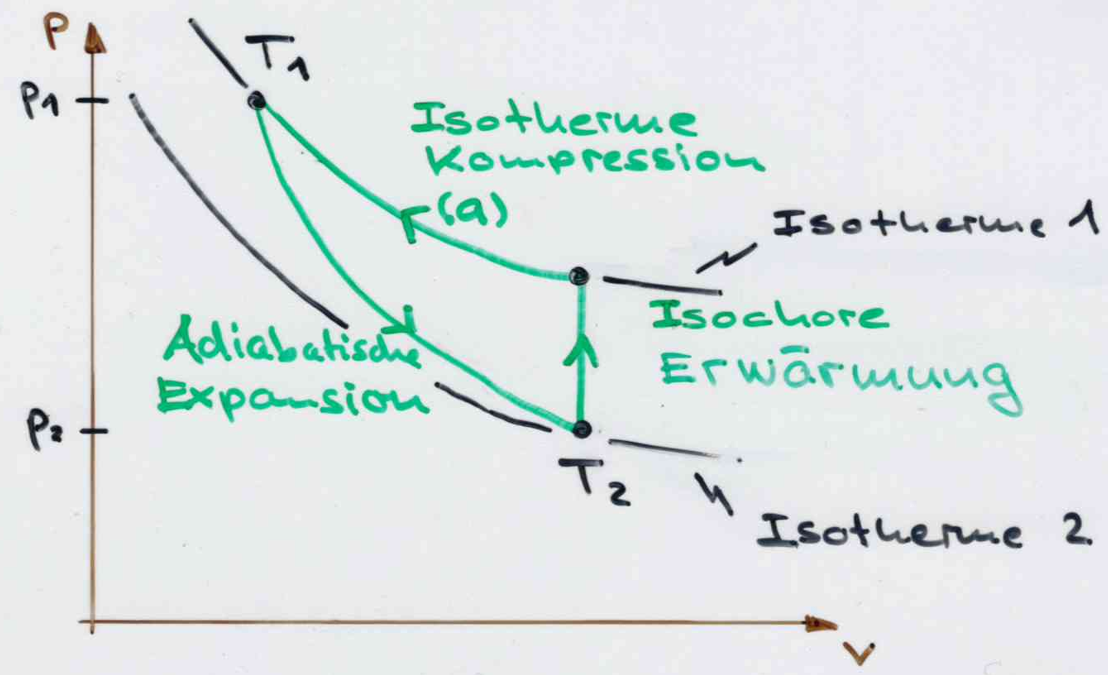
\includegraphics[width=\linewidth]{Bilder/kreisprozess}
\end{minipage}
\hfill
\begin{minipage}{0.38\linewidth}
$$ \boxed{ p \cdot V^\kappa  = \const } $$
$$ \boxed{ T \cdot V^{\kappa -1} = \const } $$
$$ \boxed{ T^\kappa \cdot p^{1-\kappa} = \const } $$
$$ \kappa = \frac{C_{mp}}{C_{mV}}$$
$$ \boxed{ C_{mp} - C_{mV} = R }$$
\\
\end{minipage}




\begin{tabular}{c l c}
	\rule{0pt}{10pt}$C_{mp}$ & Molare Wärmekapazität @ $p = \const$ & $[C_{mp}] = \mathrm{\frac{J}{mol \cdot K}}$ \\
	\rule{0pt}{10pt}$C_{mV}$ & Molare Wärmekapazität @ $V = \const$  & $[C_{mV}] = \mathrm{\frac{J}{mol \cdot K}}$ \\
	\rule{0pt}{10pt}$\kappa$ & Adiabaten-Exponent & $[\kappa] = 1$ \\
	\rule{0pt}{10pt}$R$ & Universelle Gaskonstante $R = 8.314 \mathrm{\frac{J}{mol \cdot K}}$ & $[R] = \mathrm{\frac{J}{mol \cdot K}} $ \\
\end{tabular}



\subsection{Kreisprozesse (Vorgänge)}


\begin{tabular}{lll}
isotherme Expansion & liefert Wärme & benötigt Energie \\
isotherme Kompression & benötigt Wärme & liefert Energie \\
\\
adiabatische Expansion & liefert Arbeit & ohne Wärme \\
adiabatische Kompression & benötigt Arbeit & ohne Wärme \\
\\
isochore Erwärmung & ohne Arbeit & benötigt Wärme \\
isochore Abkühlung & ohne Arbeit & liefert Wärme \\

\end{tabular}


\subsection{Beispiel Kreisprozess}
\begin{minipage}{0.48\linewidth}
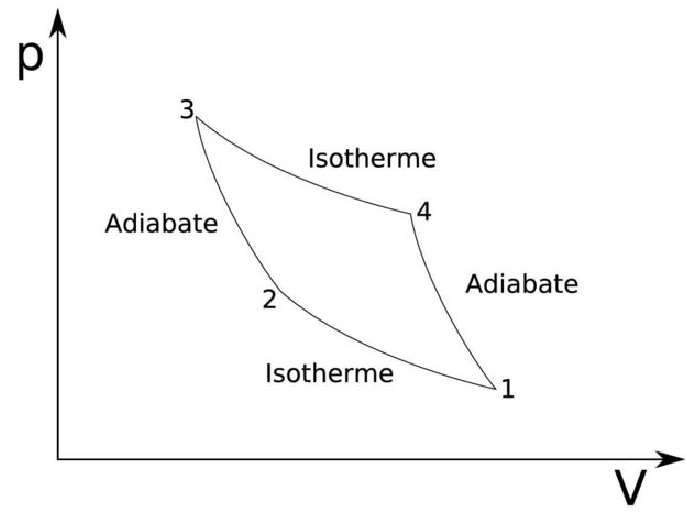
\includegraphics[width=\linewidth]{Bilder/kreisprozess_2} \\
\end{minipage}
\hfill
\begin{minipage}{0.48\linewidth}
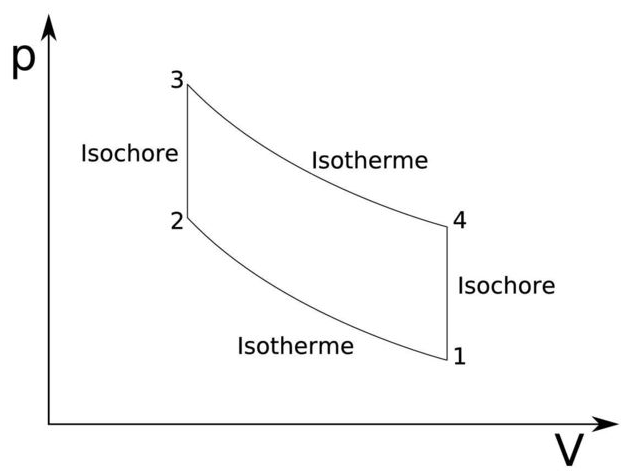
\includegraphics[width=\linewidth]{Bilder/kreisprozess_3} \\
\end{minipage}



% \vfill\null
% \columnbreak


\subsection{Entropie-Zunahme}

\subsubsection{Definition der Entropie-Zunahme}

$$ \Delta S = S_1 + S_2 = \int \frac{1}{T} \, \mathrm{d}Q  $$


\subsubsection{Boltzmann-Gleichung für Entropie-Zunahme}

$$ \boxed{ \Delta S = k \cdot \ln(W) }$$



\begin{tabular}{c l c}
	\rule{0pt}{10pt}$\Delta S$ & Entropie & $[\Delta S] = \mathrm{\frac{J}{K}}$ \\
	\rule{0pt}{10pt}$k$ & Boltzmann-Konstante $k = 1.381 \cdot 10^{-23} \mathrm{\frac{J}{K}}$ & $[k] = \mathrm{\frac{J}{K}}$ \\
	$W$ & Wahrscheinlichkeit eines Zustands & $[W] = 1$ \\
\end{tabular}


\subsubsection{Abgeschlossenes System}

\begin{tabular}{ll}
$ \Delta S \geq 0$ & Entropie kann nur zunehmen in abgeschl. System \\

$ \Delta S > 0$ & Irreversibler Prozess \\

$ \Delta S = 0$ & Reversibler Prozess \\
\end{tabular}



		\section{Molmassen wichtiger Atome}

\begin{tabular}{c | c | c }
\textbf{Symbol} & \textbf{Molekül} & \textbf{Molmasse} \\
\hline
\rule{0pt}{10pt} H & Wasserstoff & $1.008 \, \mathrm{\frac{g}{mol}}$ \\
\rule{0pt}{10pt} C & Kohlenstoff & $12.011 \, \mathrm{\frac{g}{mol}}$ \\
\rule{0pt}{10pt} N & Stickstoff & $14.007 \, \mathrm{\frac{g}{mol}}$ \\
\rule{0pt}{10pt} O & Sauerstoff & $15.999 \, \mathrm{\frac{g}{mol}}$ \\
\rule{0pt}{10pt} Al & Aluminium & $26.982 \, \mathrm{\frac{g}{mol}}$ \\
\rule{0pt}{10pt} Si & Silicium & $28.982 \, \mathrm{\frac{g}{mol}}$ \\
\end{tabular}

% \vfill\null
% \columnbreak



\section{Ansätze zu Dynamik-Aufgaben}

\subsection{Saugheber}
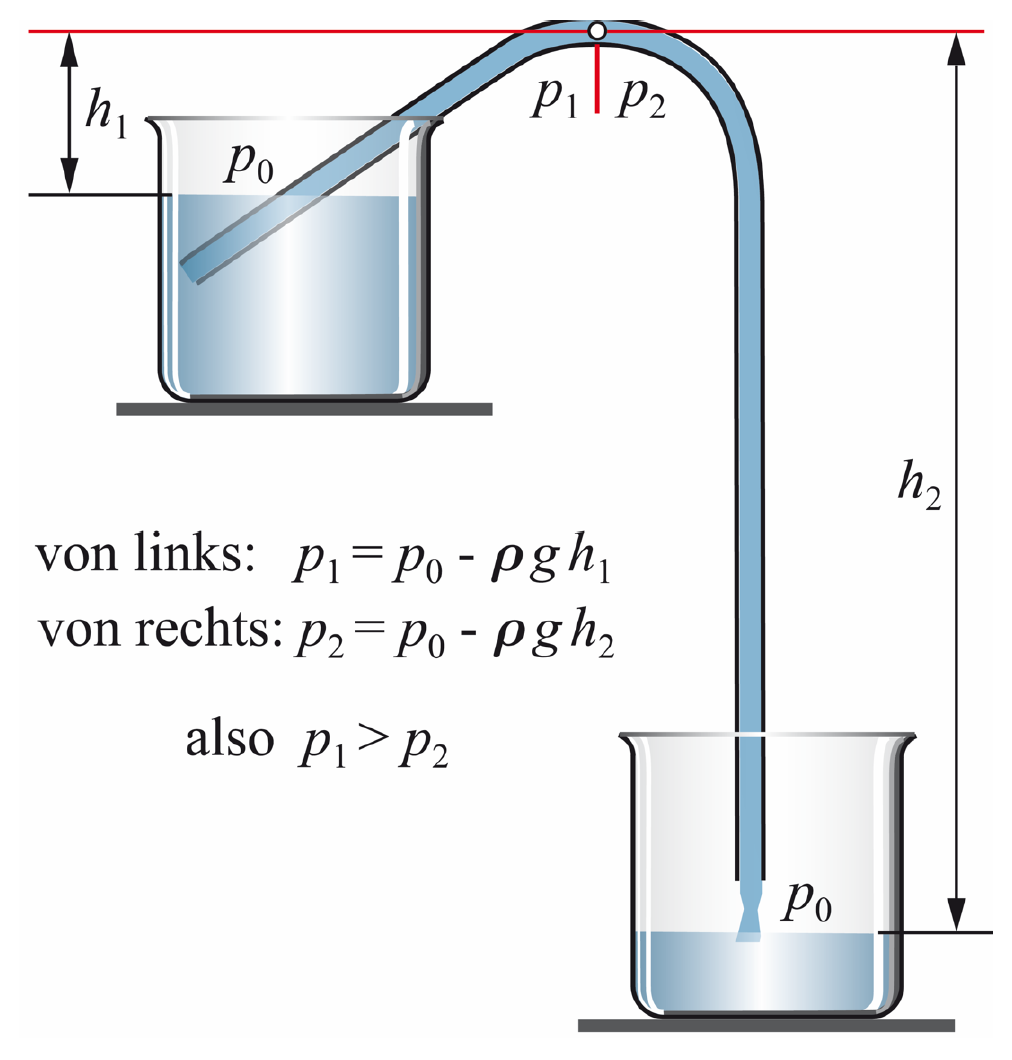
\includegraphics[width=.65\linewidth]{Bilder/saugheber.png}

\subsection{Barometer}
\begin{minipage}{0.4\linewidth}
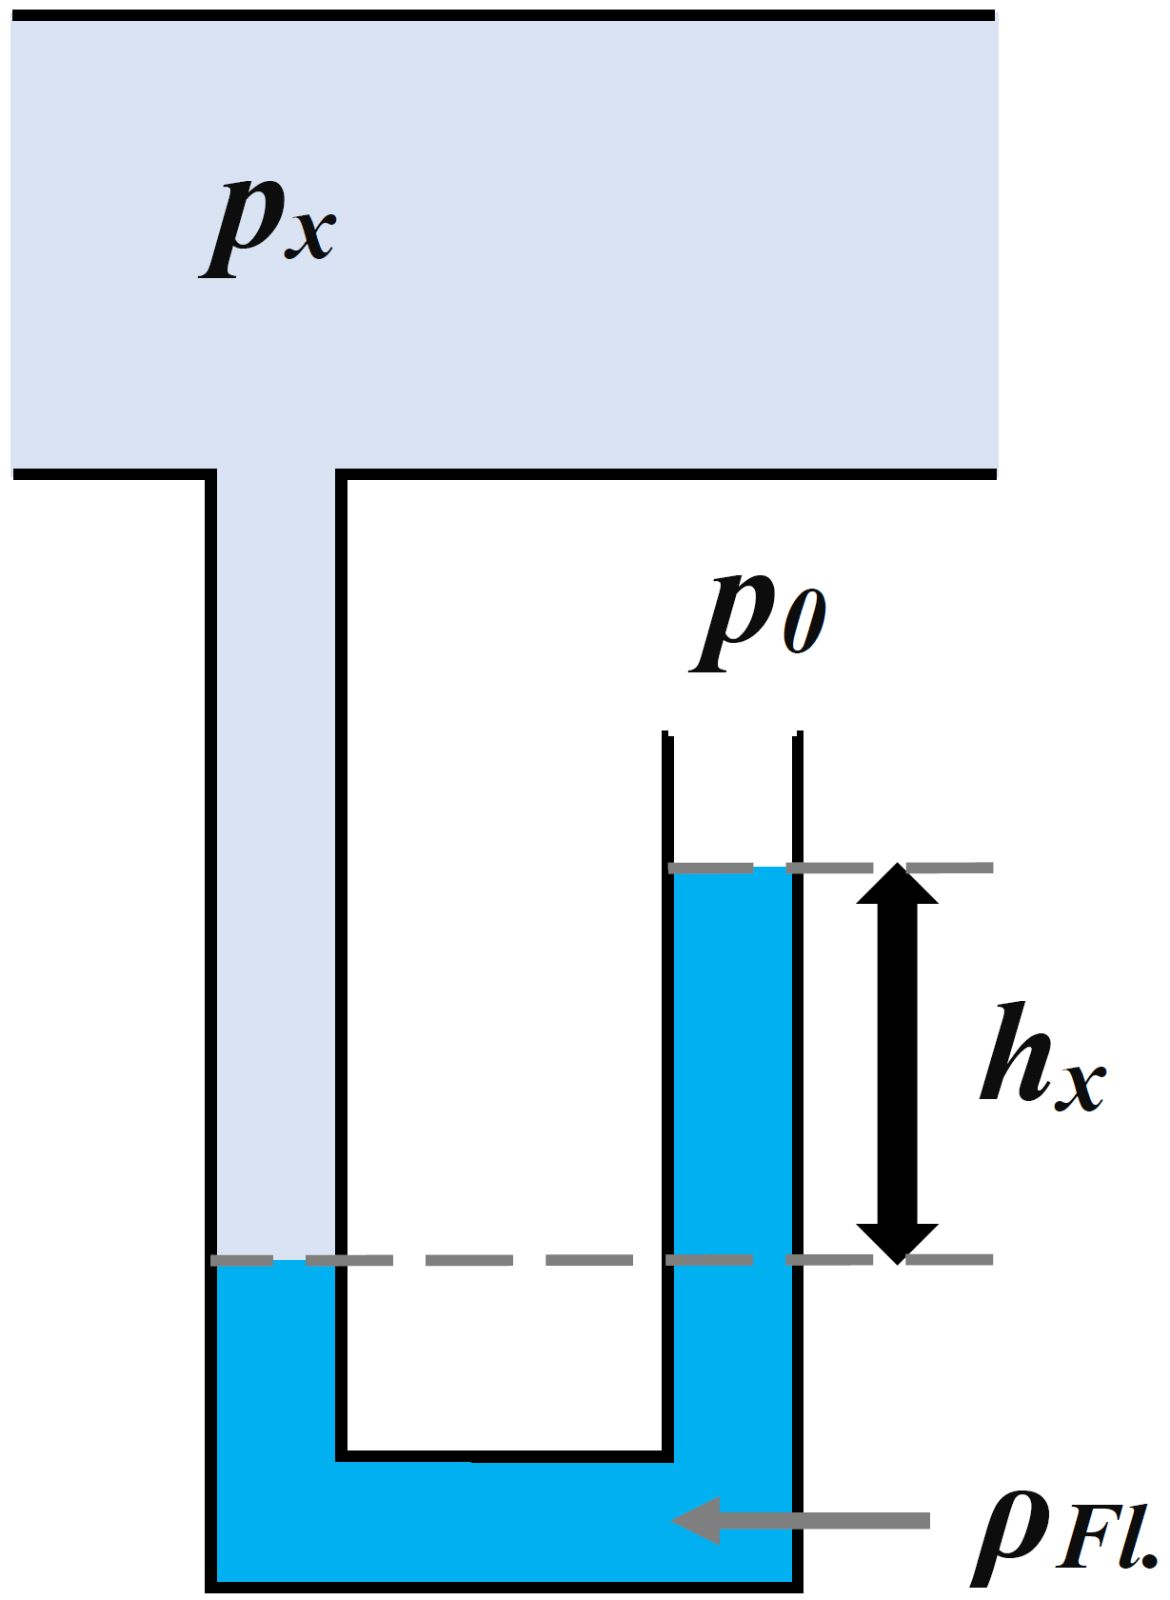
\includegraphics[width=\linewidth]{Bilder/manometer} \\
\end{minipage}
\hfill
\begin{minipage}{0.5\linewidth}
$\boxed{ p_x = p_0 + \underbrace{ \rho_{Fl} \cdot g \cdot h}_{\substack{p_s}} }$
 
 
\begin{tabular}{ll}
\\
$p_x$ & gemessener Druck \\
$p_0$ & Luftdruck \\
$p_s$ & Schweredruck \\
\\
\end{tabular}

$\Rightarrow$ Bernoulli \\
$\Rightarrow$ Kontinuität \\
\\
\\
\\
\\
\\
\end{minipage}




\subsection{Pitotrohr}
Prandtl'sches Staurohr; Staudruckmesser \\
Zur Messung von Strümungsgeschwindigkeiten \\
\\
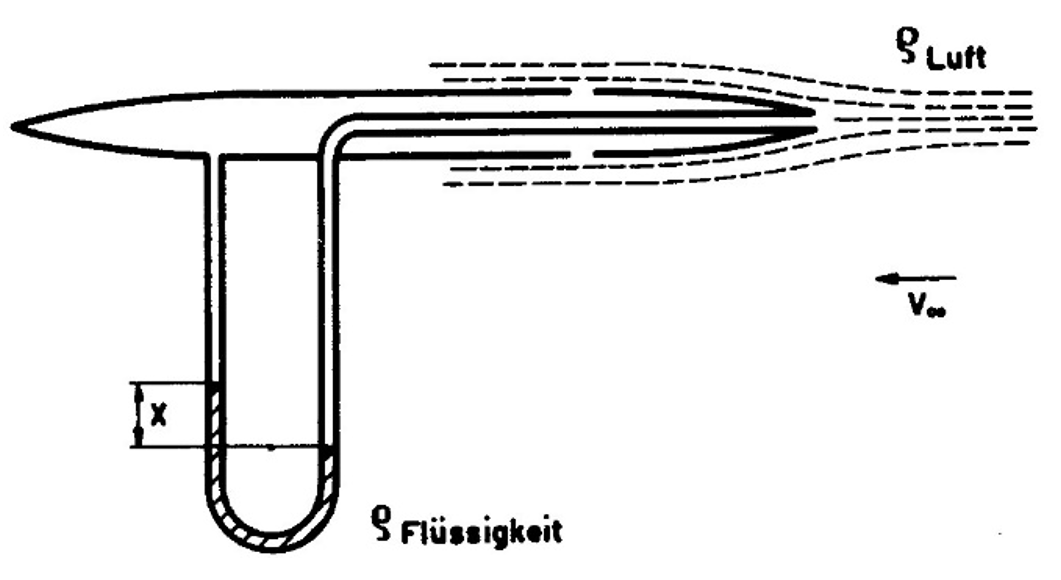
\includegraphics[width=0.7\linewidth]{Bilder/pitotrohr} \\

$$ \mathrm{Bernoulli \; horizontal:} \quad \boxed{  \underbrace{p_1}_{\substack{p_L}} + \frac{1}{2} \, \rho_1 \cdot \underbrace{v_1^2}_{\substack{0}} =  \underbrace{p_2}_{\substack{p_L - \Delta p}} + \frac{1}{2} \, \underbrace{\rho_2}_{\substack{\rho_L}} \cdot v_2^2} $$

$$ 0 = - \Delta p + \frac{1}{2} \, \rho_L \cdot v_2^2 \qquad \Rightarrow \Delta p =\frac{1}{2} \, \rho_L \cdot v_2^2 $$

$$ \mathrm{Gleichsetzen: } \quad \Delta p = \rho_{Fl} \cdot g \cdot h \quad \Rightarrow \quad v_2 = \sqrt{\frac{2 \cdot \rho_{Fl} \cdot g \cdot \Delta h}{\rho_L}} $$


\subsection{Venturirohr}
$$  \boxed{ Q = A_1 \sqrt{\frac{2 \Delta p}{\rho \left( \frac{A_1^2}{A_2^2} - 1\right)}}  \quad \quad [Q] = \frac{kg}{m^3} } $$


\subsection{Pumpe}
$$ \boxed{ W = P \cdot t = F \cdot \Delta s = p \cdot A \cdot \Delta s = p \cdot \Delta V }  $$

$$ \boxed{ P =  \frac{W}{t} = \frac{p \cdot V}{t} = p  \cdot  \dot{V} }  \quad  \boxed{ F = p \cdot A } $$



% \vfill\null
% \columnbreak


\subsection{Bewegungen}

$$ \boxed{ P = F \cdot v } \quad \boxed{ E_{kin} = \frac{1}{2} \, m \cdot v^2 } $$


\subsection{U-Rohr}

\begin{minipage}{0.4\linewidth}
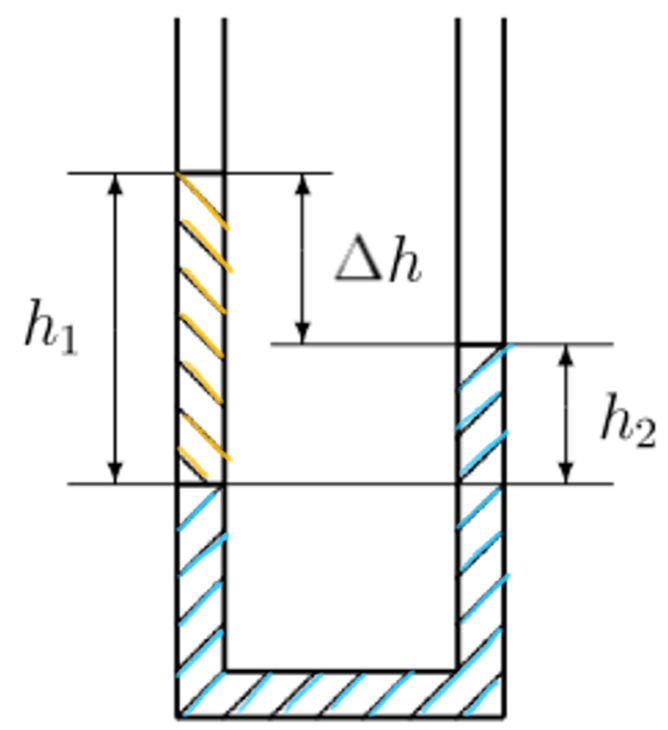
\includegraphics[width=\linewidth]{Bilder/u-rohr} \\
\end{minipage}
\hfill
\begin{minipage}{0.55\linewidth}
Ansatz: Druckgleichgewicht 

$$ p_1 = p_2 $$

$$ \rho_1 \cdot g \cdot h_1 = \rho_2 \cdot g \cdot h_2  $$
\end{minipage}


\subsection{Springbrunnen}

Ein Springbrunnen erzeugt einen $[x]$m hohen Wasserstrahl. Der Düsendurchmesser ist $[d_1]$, der Rohrdurchmesser zum Brunnen $[d_2]$, eine Pumpe für den Betrieb steht $[y]$m unterhalb des Brunnens. \\
Gesucht: Pumpdruck, Pumpenleistung bei $\eta$ = 90 $\%$\\
\\
$$\text{Bernoulli:} \quad  \overbrace{ p_1 + \frac{1}{2}\rho v_1^2}^{\text{Pumpe}} = \overbrace{p_2 + \frac{1}{2}\rho v_2^2 + \rho g y}^{\text{Düse}}, \quad v_1A_1 = v_2A_2 $$
$$ \frac{1}{2}mv^2_2 = mgx \Rightarrow v_2 = \sqrt{2gx}, \quad v_1 = v_2\frac{A_2}{A_1} = v_2\left(\frac{d_2}{d_1}\right)^2 $$
$$ \Delta p = p_1 - p_0 = \rho g y + \frac{1}{2}\rho v_2^2 - \frac{1}{2}\rho v_1^2 $$
$$ P_{ideal} = \Delta p \dot{V}, \quad P_{Pumpe} = \frac{\Delta p \dot{V}}{\eta} $$


\subsection{Wasser mit Dampf erhitzen}

Ein Tasse mit einer Masse $m_W$ Wasser und einer Temperatur von $T_K$ wird an
der Wasserdampfdüse einer Kaffeemaschine mittels Wasserdampf erhitzt. Der aus der
Kaffeemaschine ausströmende Wasserdampf ist $T_H$ heiss. Am Schluss haben sie 10 \%
mehr Wasser in der Tasse. (entspricht $m_D$)\\
Wie warm ist das Wasser nun? \\
\\
Ansatz: 1. Hauptsatz \quad $Q_{zu} = Q_{ab}$ \\
\\
$$ m_W \cdot c_W \, (T_M - T_K) = q_s \cdot m_D + m_D \cdot c_W \, (T_H - T_M) $$



\subsection{Eis in Wasser schmelzen}

In einem Gefäss befinden sich eine Masse $m_W$ Wasser. Dazu wird ein Eiswürfel mit Masse $m_E$ gegeben. Das Eis hat eine Temperatur $T_E$ und das Wasser hat eine Temperatur $T_W$. Die Temperatur $T_0$ steht für $0 \, \text{°C}$ bzw. 273.15 K \\
Gesucht ist die Mischtemperatur $T_M$ 

$$ \Delta Q_{ab} = \Delta Q_{zu}$$
$$ m_W \cdot c_W \cdot (T_W - T_M) = m_E \cdot \left( c_E \cdot (T_E - T_0) + q_f  +  c_W \cdot (T_M - T_0) \right) $$

\subsection{Beschlagenes Fenster}

Gesucht: Aussentemperatur $T_a$\\
Gegeben: Innentemperatur $T_i$, Luftfeuchtigkeit $f_i$ in $\%$, 
Wärmedurchgangszahl des Fensters $k$ und Wärmeübergangszahl $\alpha_i$\\

Beschlag bei $p_s(T_{fi}) = f \cdot p_s(T_i) \Rightarrow T_{fi} $ mittels Magnusformel bestimmen\\

Wärmestromdichte in allen Schichten gleich: $k(T_a - T_i) = \alpha_i(T_{fi} - T_i)$

\subsection{Luftbefeuchter}
Gesucht: rel. Luftfeuchtigkeit $f_{ri}$ \\
Gegeben: Volumen des Zimmers $V$, Menge verdampftes Wasser $m$, Zeit für kompletten Austausch $t$, Innentemperatur $T_i$, Aussentemperatur $T_a$, Luftfeuchtigkeit $f_{ra}$\\
$\dot{m}$ = Massenfluss (ai=nach innen, b=Befeuchter, ia=nach draussen)\\
$\dot{V} = \frac{V}{t} \quad [\frac{m^3}{s}] , \quad \quad \dot{m}_b = \frac{m}{t_0} \quad [\frac{kg}{s}], \quad \quad  M = \text{0.018} \frac{kg}{mol}$\\ 
$\rho_s = [\frac{kg}{m^3}]$ (Sättigungsdichte)

\begin{center}
    \begin{tabular}{c} 
    \\
    $ \dot{m}_{ai} + \dot{m}_b = \dot{m}_{ia} $ \\
    \\
    $ \dot{m} = f_r \cdot \rho_s \cdot \dot{V} $ \\
    \\
    $ f_{ra} \cdot \rho_{sa} \cdot \dot{V} + \dot{m}_b = f_{ri} \cdot \rho_{si} \cdot \dot{V} $ \\
    \\
    $ \rho_s = p_s (\theta) \cdot \frac{M}{R \cdot T_i} $ (Magnusformel für $p_s(T_a \text{resp.} T_i)$) \\
    \end{tabular}
\end{center}




		% \section{Vektorrechnung}
		
	\subsection{Betrag eines Vektors}
	$$ \vert \vec{A} \vert =  \sqrt{A_x^2 + A_y^2 + A_z^2}$$
		
		
	\subsection{Gleichheit zweier Vektoren}
	Zwei Vektoren sind gleich, wenn alle Komponenten identisch sind: \\
	\\
	\begin{tabular}{ll}
	$\bullet$ & $A_x = B_x$\\
	$\bullet$ & $A_y = B_y$\\
	$\bullet$ & $A_z = B_z$\\
	\end{tabular}		
		

		
		
	\subsection{Negative eines Vektors}
	\begin{minipage}{0.6\linewidth}
	\begin{tikzpicture}
		[
		x=1cm, y=1cm, scale=0.65, font=\footnotesize, >=latex 
		%Voreinstellung für Pfeilspitzen
		]
		
		%Raster links im Hintergrund
		\draw[step=1, gray, very thin] (0,0) grid (3.25,2.25);
		
		%Länge x Achse
		\draw [-latex] (0,0) -- ++(3.5,0) node[below] {$x$};
		
		%Länge y Achse
		\draw [-latex] (0,0) -- ++(0,2.5) node[left] {$y$};	
		
		%Vektor a
		\draw[-latex, red, very thick] (0.5,0.5) -- ++(2,1) node [midway, above] {$\vec{a}$} node (a) {}; 
		
		\draw[dashed] (a.center) ++ (-3,0) node (c) {};
		
		%Raster links im Hintergrund
		\draw[step=1, gray, very thin] (4,0) grid (7.25,2.25);
		
		%Länge x Achse
		\draw [-latex] (4,0) -- ++(3.5,0) node[below] {$x$};
		
		%Länge y Achse
		\draw [-latex] (4,0) -- ++(0,2.5) node[left] {$y$};	
		
		%Vektor a
		\draw[-latex, red, very thick] (6.5,1.5) -- ++(-2,-1) node [midway, above] {$\vec{b}$} node (a) {}; 
		
	\end{tikzpicture}
	\end{minipage}
	\hfill
	\begin{minipage}{0.3\linewidth}
	$b_x = - a_x$ \\
	\\
	$b_y = - a_y$ \\
	\\
	$b_z = - a_z$ \\
	\end{minipage}	
		
		
	
	\subsection{Addition zweier Vektoren}
	
	\begin{minipage}{0.6\linewidth}
	\begin{tikzpicture}
		[
		x=1cm, y=1cm, scale=0.7, font=\footnotesize, >=latex 
		%Voreinstellung für Pfeilspitzen
		]
		
		%Raster im Hintergrund
		\draw[step=1, gray, very thin] (0,0) grid (5.5,3.5);
		
		%Zahlen auf x-Achse
		\foreach \x in {0,1,2,3,4,5}
		\draw[shift={(\x,0)},color=black] (0pt,2pt) -- (0pt,-2pt) node[below]
		{\footnotesize $\x$};
		%Länge x Achse
		\draw [-latex] (0,0) -- ++(5.5,0) node[below] {$x$};
		%Länge y Achse
		\draw [-latex] (0,0) -- ++(0,3.5) node[left] {$y$};
		
		%Zahlen auf y-Achse
		%\foreach \y in {0,...,1}
		\foreach \y in {0,1,2,3}
		\draw[shift={(0,\y)},color=black] (2pt,0pt) -- (-2pt,0pt) node[left]
		{\footnotesize $\y$};		
		
		%Vektor a
		\draw[-latex, thick] (0,0) -- (2,3) node [midway, above] {$\vec{a}$} node (a) {}; 
		%Vektor b
		\draw[-latex, thick] (0,0) -- (3,0) node [midway, above] {$\vec{b}$} node (b) {}; 
		\draw[dashed] (a.center) -- ++ (3,0) node (c) {};
		\draw[dashed] (b.center) -- ++ (2,3);
		\draw[very thick, red, -latex] (0,0) -- (c.center) node [midway, above] {$\vec{c}$};
	\end{tikzpicture}
	\end{minipage}
	\hfill
	\begin{minipage}{0.3\linewidth}
	$c_x = a_x + b_x$ \\
	\\
	$c_y = a_y + b_y$ \\
	\\
	$c_z = a_z + b_z$ \\
	\end{minipage}
	
	
		
		
		
	\subsection{Subtraktion zweier Vektoren}
	
	\begin{minipage}{0.6\linewidth}
	\begin{tikzpicture}
		[
		x=1cm, y=1cm, scale=0.8, font=\footnotesize, >=latex 
		%Voreinstellung für Pfeilspitzen
		]
		
		%Raster im Hintergrund
		\draw[step=1, gray, very thin] (-0.5,-0.5) grid (6.5,2.5);
		
		%Zahlen auf x-Achse
		%\foreach \x in {0,1,2,3}
		%\draw[shift={(\x,0)},color=black] (0pt,2pt) -- (0pt,-2pt) node[below]
		%{\footnotesize $\x$};
		
		%Länge x Achse
		\draw [-latex] (0,0) -- (6.5,0) node[below] {$x$};
		
		%Länge y Achse
		\draw [-latex] (0,0) -- ++(0,2.5) node[left] {$y$};	
		
		%Vektor a
		\draw[-latex, very thick] (0,0) -- (3,2) node [midway, above] {$\vec{a}$} node (a) {}; 
		
		%Vektor b
		\draw[-latex, dashed, very thick] (3,2) -- ++(3,0) node [midway, above] {$\vec{b}$} node (b) {};
		\draw[-latex, very thick, blue] (3,2) -- ++(-3,0) node [midway, above] {$-\vec{b}$} node (-b) {}; 
		\draw[dashed] (a.center) ++ (-3,0) node (c) {};
		
		%\draw[dashed] (-b.center) -- ++ (2,3);
		%\draw[dashed] (b.center) -- ++ (-1,3);
		\draw[very thick, red, -latex] (0,0) -- (c.center) node [midway, left] {$\vec{c}$};
		
		%Zahlen auf y-Achse 
		%\foreach \y in {0,...,1}
		%\foreach \y in {1,2,3}
		%\draw[shift={(0,\y)},color=black] (2pt,0pt) -- (-2pt,0pt) node[left]
		%{\footnotesize $\y$};	
	\end{tikzpicture}
	\end{minipage}
	\hfill
	\begin{minipage}{0.3\linewidth}
	$c_x = a_x - b_x$ \\
	\\
	$c_y = a_y - b_y$ \\
	\\
	$c_z = a_z - b_z$ \\
	\end{minipage}	
		
		
	\subsection{Multiplikation eines Vektros mit einem Skalar}
	\begin{minipage}{0.68\linewidth}
	$$\vec{b} = s \, \vec{a} \quad \vert \vec{B} \vert = \vert s \vert \cdot \vert \vec{a} \vert$$ \\
	\end{minipage}
	\hfill
	\begin{minipage}{0.3\linewidth}
	$b_x = s \cdot a_x$ \\
	\\
	$b_y = s \cdot a_y$ \\
	\\
	$b_z = s \cdot a_y$ \\
	\end{minipage}	
	
		
		
		
		
	\subsection{Skalarprodukt}
	$$\vec{c} = \vec{a} \bullet \vec{b} = \vert \vec{a} \vert \cdot \vert \vec{b} \, \vert  \, \cos(\varphi)$$ 
		
		
		
		
		
	\subsection{Kreuzprodukt (nur in 3D)}
	 $$\vec{a} \times \vec{b} = \begin{pmatrix} a_2 b_3 - a_3 b_2 \\ -(a_1 b_3 - a_3 b_1) \\ a_1 b_2 - a_2 b_1 \end{pmatrix}$$ 
		
				


		% \section{Statistik}
	\subsection{Arithmetisches Mittel $\overline{x}_{arith}$}
		
	$\overline{x}_{arith} := \frac{1}{N} \sum \limits_{i = 1}^N  x_i$
	
		
		
	\subsection{Geometrisches Mittel $\overline{x}_{geom}$}
	\textbf{Nur für positive Zahlenreihen $x_i$ definiert!} \\
	\\		
	$\overline{x}_{geom} := \sqrt[N]{\prod \limits_{i = 1}^N  x_i }$ \qquad \qquad $\Rightarrow \overline{x}_{geom} \leq \overline{x}_{arith}$
		
		
		
	\subsection{Quadratisches Mittel QMW (RMS)}
	\textbf{Wechselstromtechnik; Effektivwert} \\
	\\
	$QMW := \sqrt{ \frac{1}{N} \sum \limits_{i = 1}^N  x_i^2 }$
		
		
	\subsection{Harmonisches Mittel $\overline{x}_{harm}$}		
	
	$\overline{x}_{harm} := \frac{N}{ \sum \limits_{i = 1}^N   \frac{1}{x_i} } $ \\
	\\
	Kann sinnvoll eingesetzt werden, wenn man für die $i-te$ Teilstrecke $s_i$ eine Zeit $t_i$ benötigt (also eine Durchschnittsgeschwindigkeit von $v_i = \frac{s_i}{t_i}$ und eine Durchschnittsgeschwindigkeit über $N$ Teilstrecken ermitteln will: \\
	\\
	$\overline{v}_{harm} = \frac{\sum \limits_{i = 1}^N  s_i }{\sum \limits_{i = 1}^N  t_i} = \frac{\sum \limits_{i = 1}^N  s_i }{\sum \limits_{i = 1}^N \frac{s_i}{v_i} }  $ \qquad gewichtetes harm. Mittel
		
		
		
	\subsection{Standardabweichung $\sigma$}	
		
	\begin{tabular}{ll}
	Varianz: & $\sigma^2 := \frac{1}{N} \sum \limits_{i = 1}^N (x_i - \overline{x}_{arith} )^2 $ \\
	\\
	Standardabweichung: &  $\sigma := \sqrt{ \frac{1}{N} \sum \limits_{i = 1}^N (x_i - \overline{x}_{arith} )^2 }$ \\
	\end{tabular}
		
		
		
	\subsection{Standardabweichung des Mittelwerts}	
	\textbf{Gilt nur, wenn eine Normalverteilung vorliegt!} \\
	Beschreibt nur statistische Fehler \\
	\\
	$\sigma(\overline{x}_{arith}) = \frac{\sigma}{\sqrt{N}} $
		
		

		% \section{Mathematik-Hilfe}
		
	\subsection{Trigonometrie}
	\begin{tabular}{| c | c | c |}
	\hline
	Sinus & Cosinus & Tangens \\ 
	\hline 
	\rule{0pt}{10pt} $\frac{GK}{H}$ & $\frac{AK}{H}$ & $\frac{AK}{GK}$ \\ 
	\hline
	\end{tabular} 
		
		
		
	\subsection{Schwerpunkt}
	Die Koordinaten des Schwerpunkts müssen komponentenweise berechnet werden: \\
	\\
	$x_s = \frac{\sum  x_i \cdot m_i}{M}$ \qquad	$y_s = \frac{\sum  y_i \cdot m_i}{M}$ \qquad $z_s = \frac{\sum  z_i \cdot m_i}{M}$ \\
	\\
	\begin{tabular}{ll}
	$x_s \; , y_s \; , z_s$ & Koordinaten des Schwerpunkts \\
	$x_i \; , y_i \; , z_i$ & Koordinaten von kleinen Massepunkten \\
	$m_i$ & Kleine Massepunkte an entsprechenden Koordinaten \\
	$M$ & Gesamtmasse des Körpers
	\end{tabular}
	
	\subsection{Polarkoordinaten (Kreisbewegung)}

	
	\begin{tabular}{ll}
	polar $\rightarrow$ kartesisch & $\vec{P} =  \begin{pmatrix} x \\ y \end{pmatrix} =  \begin{pmatrix} r \cdot \cos(\phi)  \\ r \cdot \sin(\phi)  \end{pmatrix}$ \\
	\\
	kartesisch $\rightarrow$ polar & $\vec{P} =  \begin{pmatrix} r \\ \phi \end{pmatrix} =  \begin{pmatrix} \sqrt{x^2 + y^2}  \\ \tan \big( \frac{x}{y} \big)   \end{pmatrix}$\\
	\end{tabular}
	
	
	
	\subsection{Ableitungsregeln S .445-448}
			
			\subsubsection{Elementare Regeln}
			\begin{tabular}{lll}
			Potenzen: & $f(x) = x^3$ & $f'(x) = 3 \, x^2$ \\
			& $f(x) = x^\alpha$ & $f'(x) = \alpha \cdot x^{\alpha - 1}$ \\
			\\
			Linearität: & $f(x) = c \cdot x^2$ & $f'(x) = c \cdot 2 \, x $ \\
			\\
			Summe: & $(u(x) + v(x) - w(x))' $ & = $u'(x) + v'(x) - w'(x)$ \\
			\\
			Konstanten: & $c = const$ $\rightarrow$ $c' = 0$ \\
			\end{tabular}
			
			
			\subsubsection{Produktregel}
			$(f(x) \cdot g(x))' = f'(x) \cdot g(x) + f(x) \cdot g'(x)$ 
			
			\subsubsection{Quotientenregel}
			$\left( \frac{u(x)}{v(x)} \right) ' = \frac{u'(x) \cdot v(x) - u(x) \cdot v'(x)}{v(x) ^2}$ \quad $\rightarrow$ als Produkt schreiben \\
			\\
			$u(x) \cdot \left( \frac{1)}{v(x)} \right) ' =  u'(x) \cdot \frac{1}{v(x)} + u(x) \cdot \frac{- v'(x)}{v(x)^2}$
			
			\subsubsection{Kettenregel}
			$g(f(x))' =  f'(x) \cdot g'(x)$ \\
			
			\subsubsection{Umkehrfunktion}
			$(f^{-1}(y_0))' = \frac{1}{f'(x_0)} =  \frac{1}{f'(f^{-1}(y_0))}$ \\
			

			
			\subsection{Allgemeine Logarithmus-Ableitung}
			$(\log_b(x))' = \left( \frac{\ln(x)}{\ln(b)} \right)' = \frac{1}{\ln(b)} \cdot (\ln(x))' = \frac{1}{\ln(b)} \cdot \frac{1}{x} $
			
			
			
			
			\subsection{Integrationsregeln S. 494-496}
		Linearität: $\int \limits_{a}^{b} \alpha \, f(x) \, dx = \alpha \int \limits_{a}^{b} f(x) \, dx$ 
		
		
		\subsubsection{Rechenregeln mit Integralen S. 508-510}
		\begin{tabular}{ll}
		Zerlegung: & $\int \limits_{a}^{b} f_1(x) \, dx + f_2(x) \, dx = \int \limits_{a}^{b} f_1(x) \, dx + \int \limits_{a}^{b} f_2(x) \, dx$ \\
		\\		
		& $\int \limits_{a}^{c} f(x) \, dx = \int \limits_{a}^{b} f(x) \, dx + \int \limits_{b}^{c} f(x) \, dx$ \\
		\\
		Grenzen tauschen: & $ \int \limits_{a}^{b} f(x) \, dx = -  \int \limits_{b}^{a} f(x) \, dx $ \\
		\\
		Gleiche Grenzen: &  $\int \limits_{a}^{a} f(x) \, dx = 0$ \\
		\end{tabular}
		
		
		\subsection{Wichtige Integrale S. 495}
		\begin{tabular}{ll}
		$\int \limits_{a}^{b} x^2  \, dx = \frac{b^3}{3} - \frac{a^3}{3}$ & $\int \limits_{a}^{b} x \, dx = \frac{b^2}{2} - \frac{a^2}{2}$ \\
		\\
		$\int \limits_{a}^{b} 1 \, dx = b - a $ (Rechteck)& \\
		\end{tabular}
			
	
	
		
	\end{multicols*}	
\end{document}